\documentclass{beamer}


\usepackage[spanish]{babel} 
\usepackage[utf8]{inputenc} 
\usepackage{amsmath}
\usepackage{hyperref}
\usepackage[nodayofweek]{datetime}
\usepackage{pgfpages}

\usepackage{caption}
\usepackage{subcaption}


\makeatletter
\def\verbatim@font{\ttfamily\tiny}
\makeatother

%~ \usetheme{Berkeley}
%~ \usetheme{CambridgeUS} %~ Ok 3
%~ \usetheme{Boadilla} %~ Ok 2
\usetheme{boxes} %~ Ok 1
\setbeamerfont{frametitle}{size=\small}

\usecolortheme{seahorse} %~ OK
%~ \usecolortheme{dolphin} 
%~ \usecolortheme{beaver}
%~ \usecolortheme{whale}
%~ \usecolortheme{lily}


%~ \usetheme{Frankfurt}
%~ \usetheme{Madrid}
%~ \usetheme{Malmoe}

%~ \setbeamercovered{transparent}

\logo{%
	   
\includegraphics[scale=.25]{img/logoIBR2016_byn.png}
   }
\title[]{Estudios sobre la regulación de la expresión génica por microARNs en plantas mediante estrategias bioinformáticas}

\author{Uciel Chorostecki}
\institute[IBR]{ \\Director Dr. Javier Palatnik\\Instituto Biología Molecular y Celular Rosario}
\date{}

\begin{document}

\frame{\titlepage}

\section{Introducción}

\begin{frame}{miARNs}
    \begin{itemize}
        \item Los microARNs (miARNs) son ARN pequeños de 20-22 nt que regulan la expresión génica en animales y plantas. 
        \item En plantas controlan procesos vitales como el desarrollo, señalización hormonal y respuestas al estrés
    \end{itemize}
\end{frame}

\section{Objetivos}

\begin{frame}{Objetivos}
    \setbeamercovered{transparent=25}
	\begin{enumerate}[<+->]
        \item Identificar genes regulados por miARNs en plantas.
        \item Estudiar la biogénesis de los miARNs en plantas.
	\end{enumerate}
\end{frame}

\begin{frame}{Objetivos específicos}
    \setbeamercovered{transparent=25}
		\pause
		\begin{itemize}
            \item<-2> Diseñar una estrategia y una herramienta web para la identificación de genes blancos regulados por miARNs en plantas.
			\item<-1> Desarrollar herramientas para el análisis de los intermediarios de procesamiento de miARNs en plantas.
			\item<-1> Identificar y caracterizar precursores de miARNs en distintas especies que tengan mecanismos de procesamiento distintos.
			\item<-1> Caracterizar la relación entre la evolución de los precursores de miARNs en plantas y los mecanismos de procesamiento determinados previamente.
        \end{itemize}
\end{frame}


\section{Resultados}

\subsection{Resultados 1}

\begin{frame}{Aplicaciones bioinformáticas para el estudio de interacciones miARN-gen blanco}
\end{frame}

\begin{frame}{Conservación y divergencia de miARNs en distintas especies}
	\begin{center}
		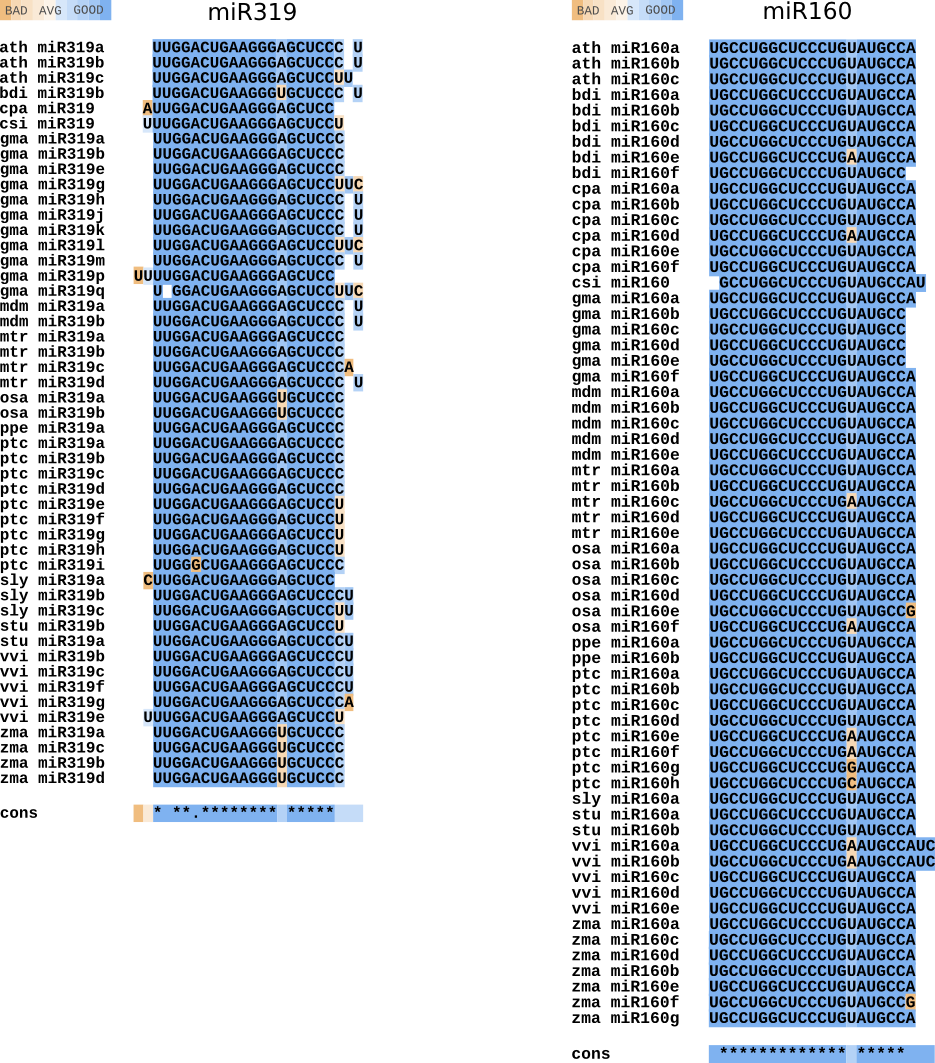
\includegraphics[width=0.5\textwidth]{img/variabilidad_maduro.png}
	\end{center}
\end{frame}

\begin{frame}{22 miARNs que están conservados en Angiospermas}
	\begin{center}
		
\includegraphics[width=0.5\textwidth]{img/NAR_fig1_01.png}
	\end{center}
\end{frame}

\begin{frame}{Secuencias consensos de 18 nt (2-19)}
	\begin{center}
		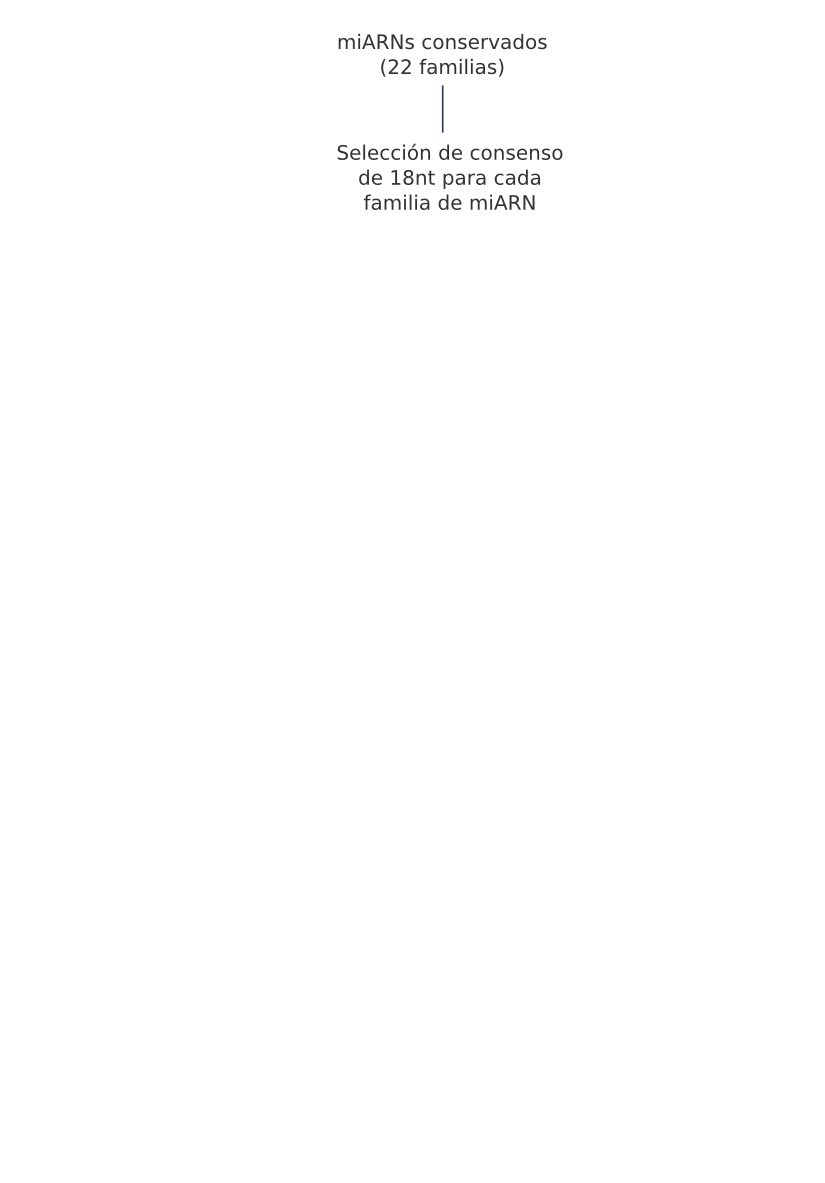
\includegraphics[width=0.5\textwidth]{img/NAR_fig1_02.png}
	\end{center}
\end{frame}

\begin{frame}{Primera búsqueda general de potenciales genes blancos}
	\begin{center}
		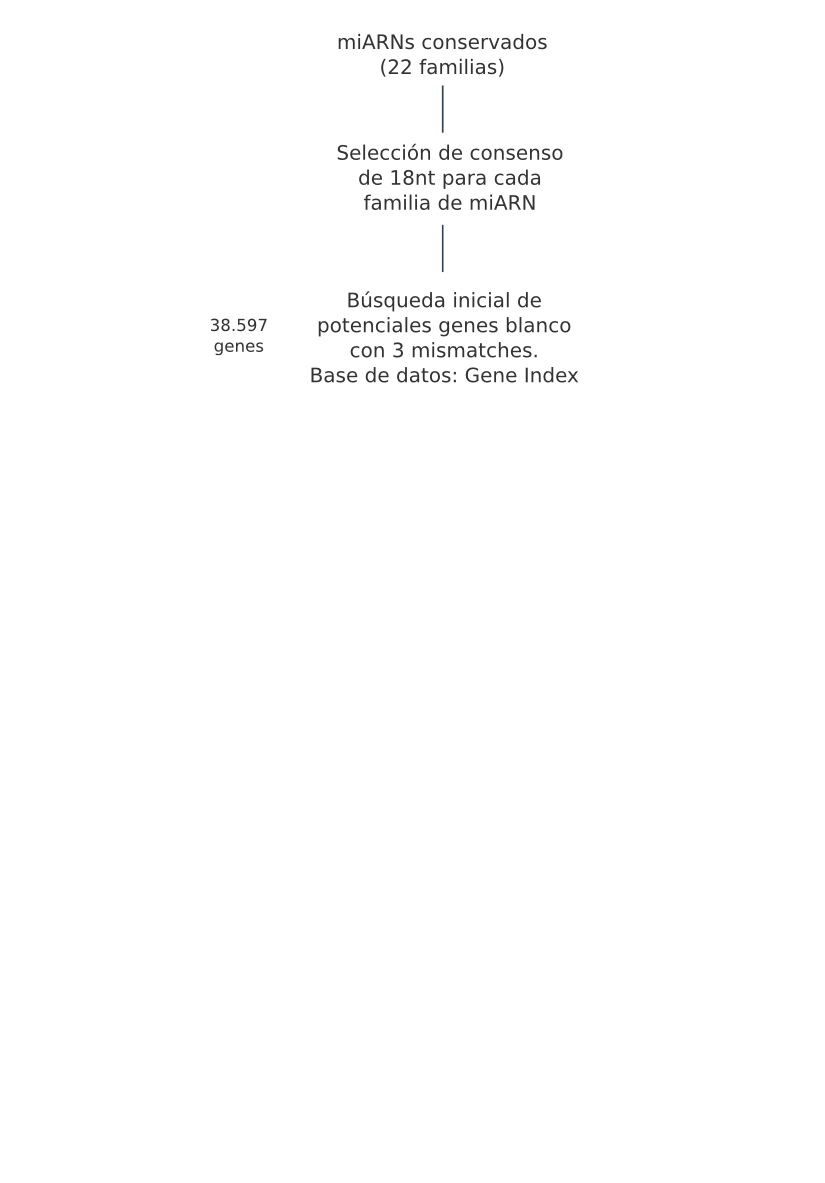
\includegraphics[width=0.5\textwidth]{img/NAR_fig1_03.png}
	\end{center}
\end{frame}

\begin{frame}{Filtros de evolución y empíricos de interacción miARN-gen blanco}
	\begin{center}
		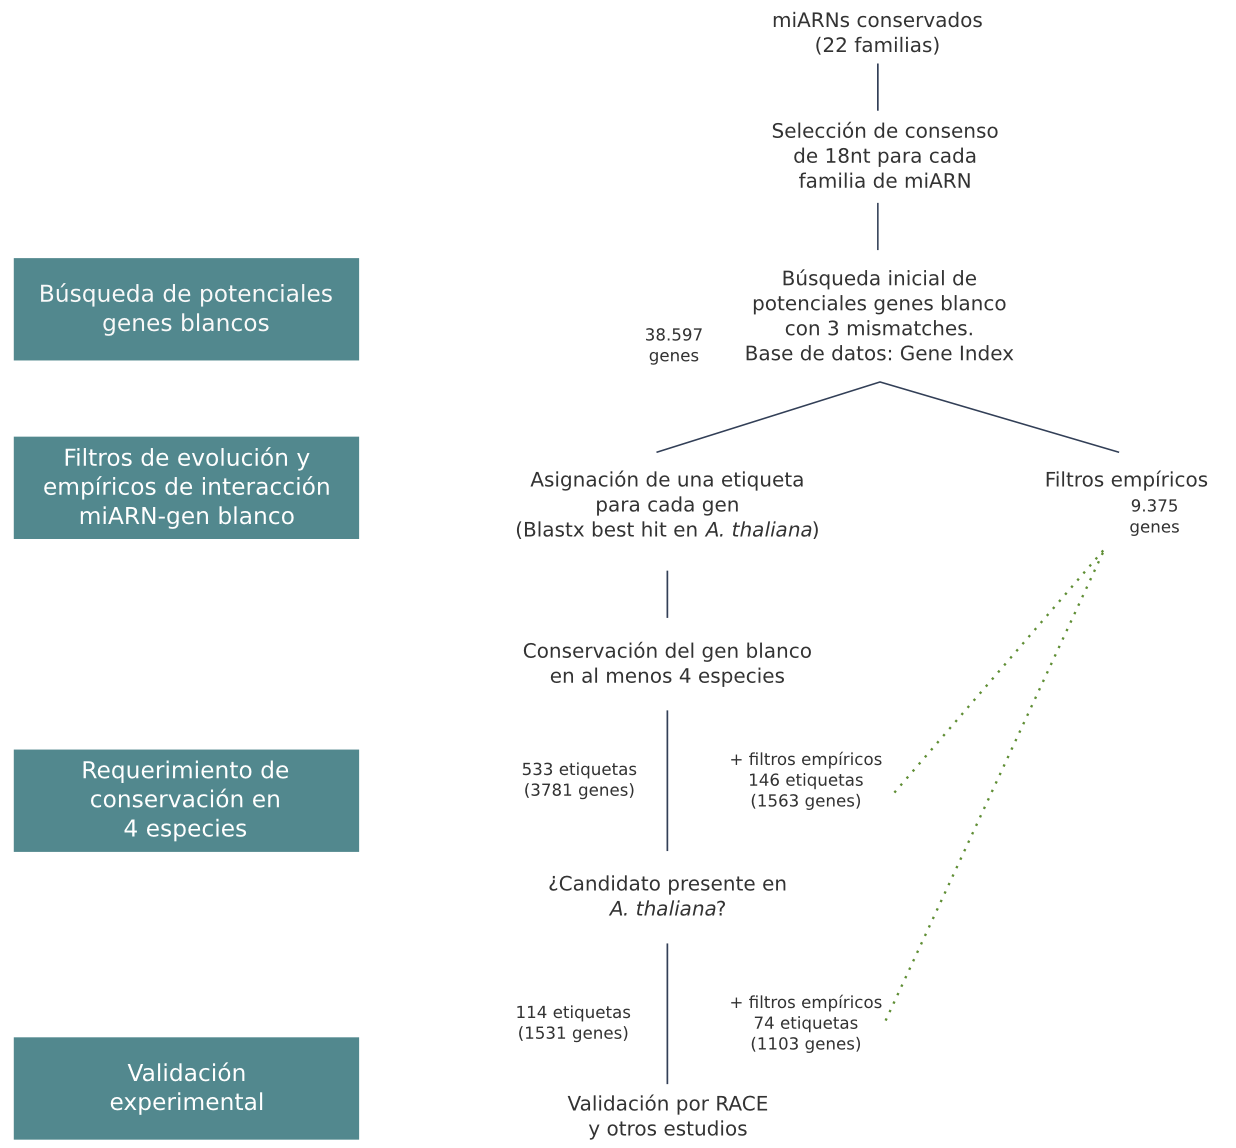
\includegraphics[width=0.5\textwidth]{img/NAR_fig1_04.png}
	\end{center}
\end{frame}

\begin{frame}{Mínimo de 4 especies requeridas}
	\begin{center}
		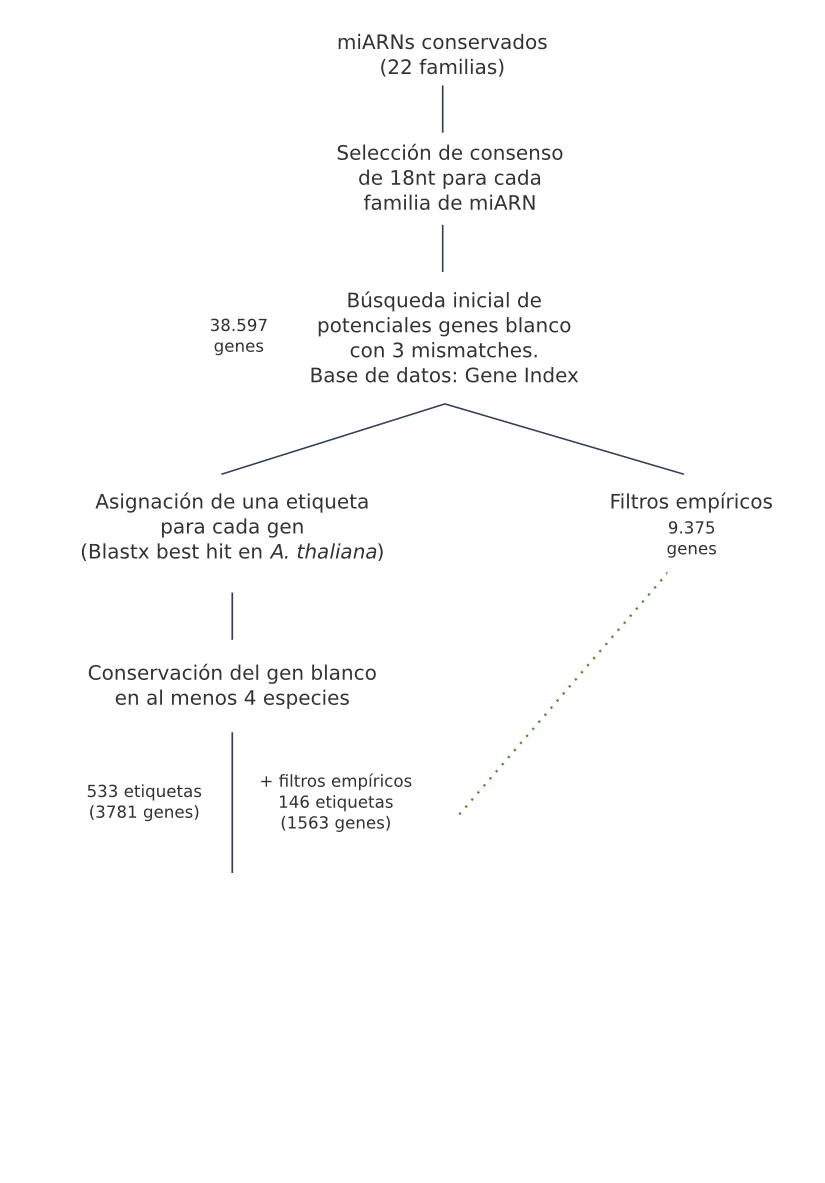
\includegraphics[width=0.5\textwidth]{img/NAR_fig1_05.png}
	\end{center}
\end{frame}

\begin{frame}{Genes blancos en \textit{A. thaliana}}
	\begin{center}
		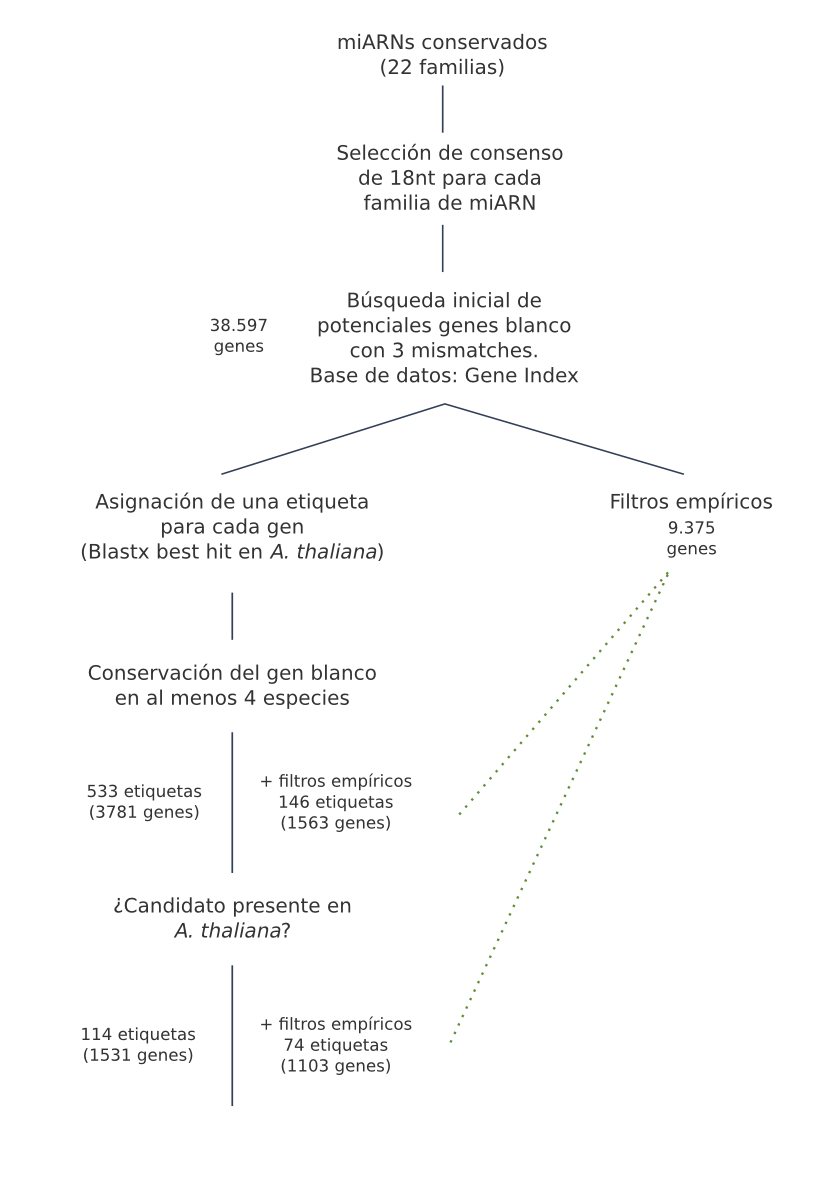
\includegraphics[width=0.5\textwidth]{img/NAR_fig1_06.png}
	\end{center}
\end{frame}

\begin{frame}{Validación experimental}
	\begin{center}
		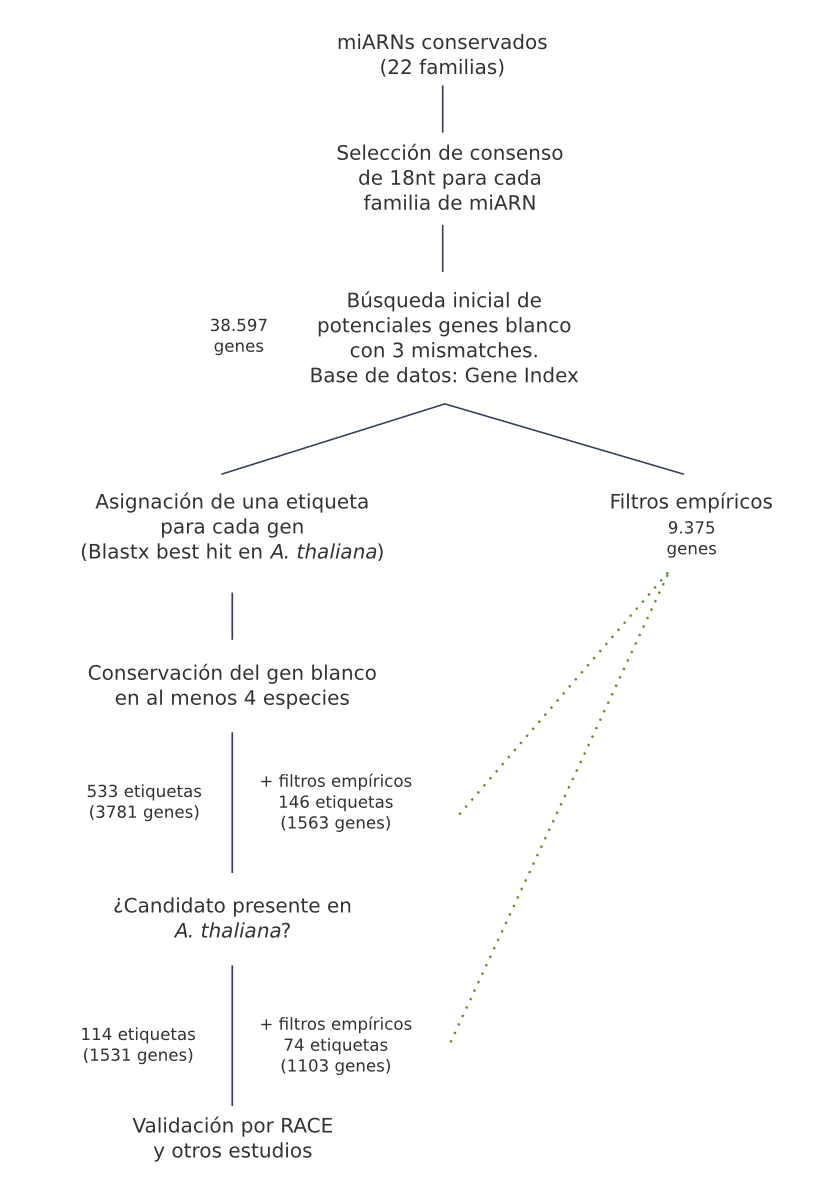
\includegraphics[width=0.5\textwidth]{img/NAR_fig1_07.png}
	\end{center}
\end{frame}

\begin{frame}{Conservación de la interacción en distintas especie}
	\begin{center}
		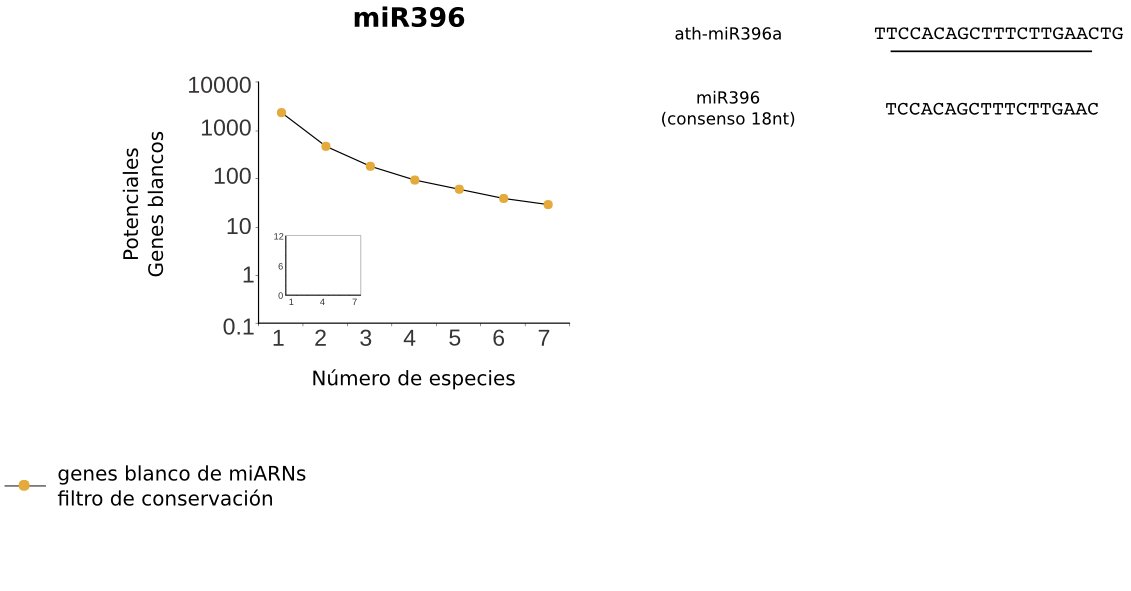
\includegraphics[width=0.5\textwidth]{img/NAR_fig2_01.png}
	\end{center}
\end{frame}

\begin{frame}{La relación señal/ruido incrementa al aumentar el número de especies}
	\begin{center}
		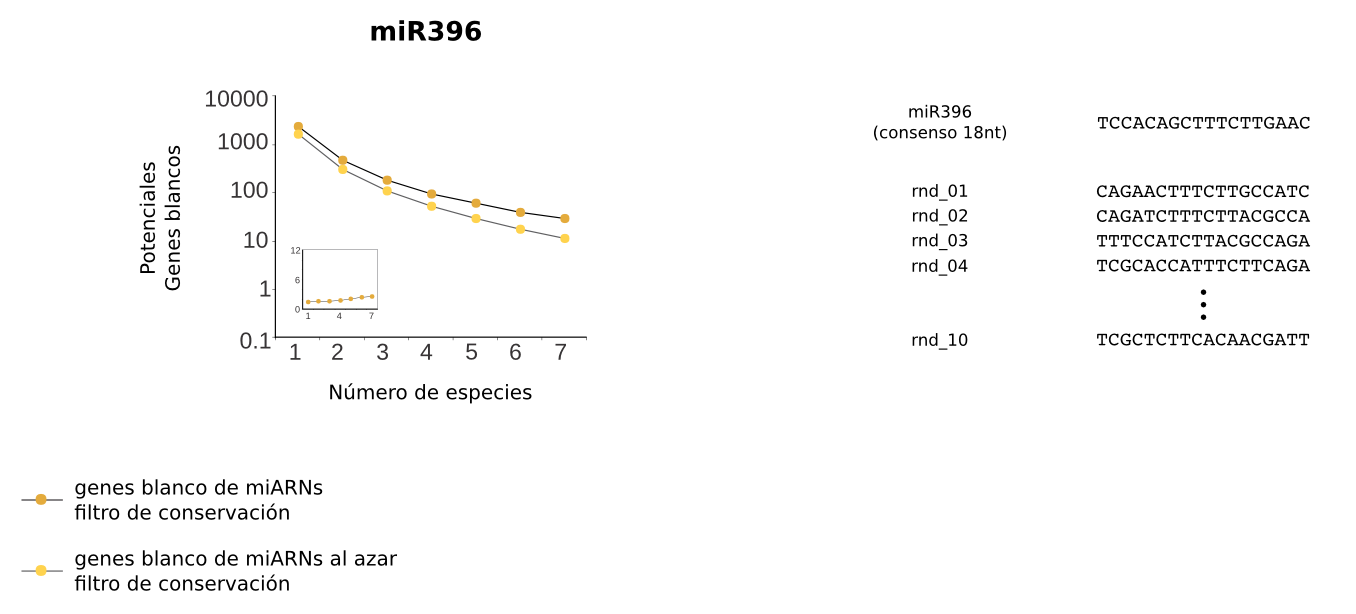
\includegraphics[width=0.5\textwidth]{img/NAR_fig2_02.png}
	\end{center}
\end{frame}

\begin{frame}{Slección de candidatos teniendo en cuenta los filtros empíricos}
	\begin{center}
		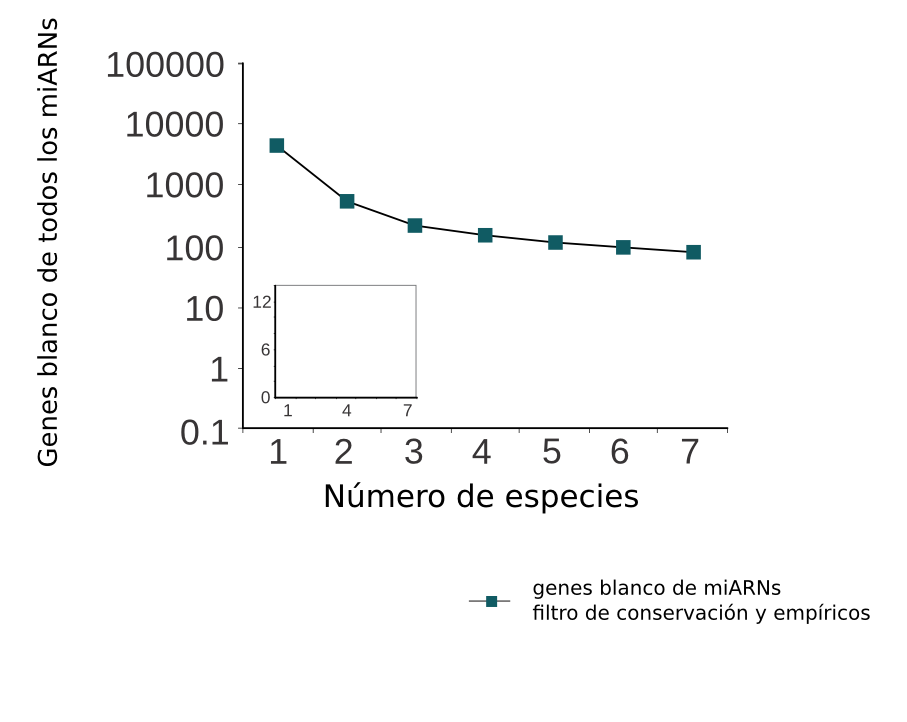
\includegraphics[width=0.5\textwidth]{img/NAR_fig2_03.png}
	\end{center}
\end{frame}

\begin{frame}{Al aplicar filtros empíricos y de conservación la relación señal/ruido aumenta}
	\begin{center}
		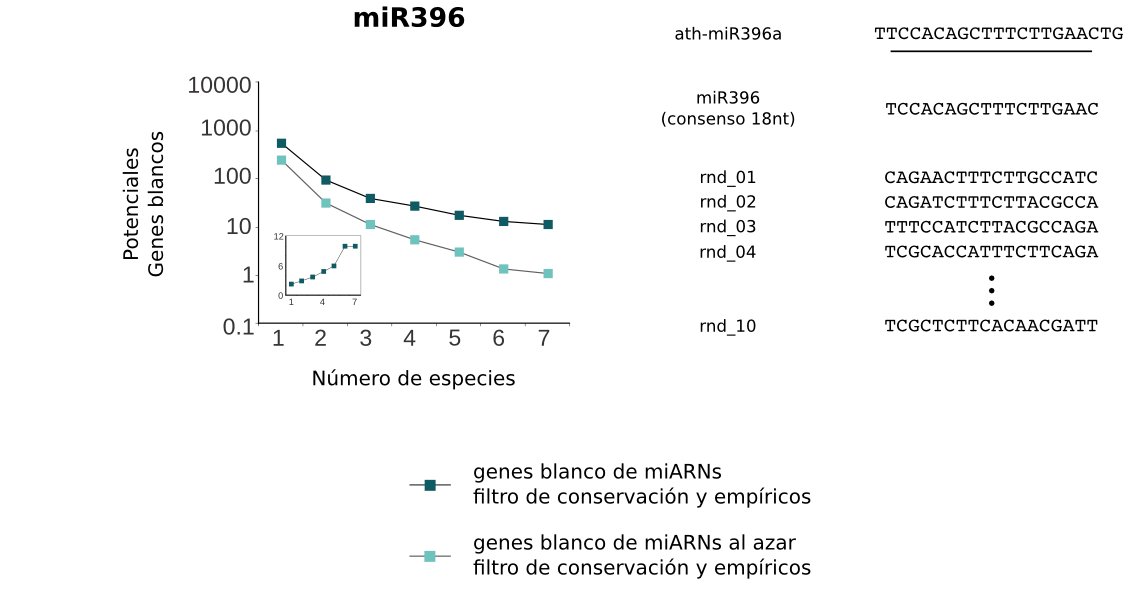
\includegraphics[width=0.5\textwidth]{img/NAR_fig2_04.png}
	\end{center}
\end{frame}

\begin{frame}{Efecto sinérgico al combinar filtro de conservación evolutiva y empíricos}
%~ pueden estar seleccionando aspectos diferentes de la interacción miARN-gen blanco
	\begin{center}
		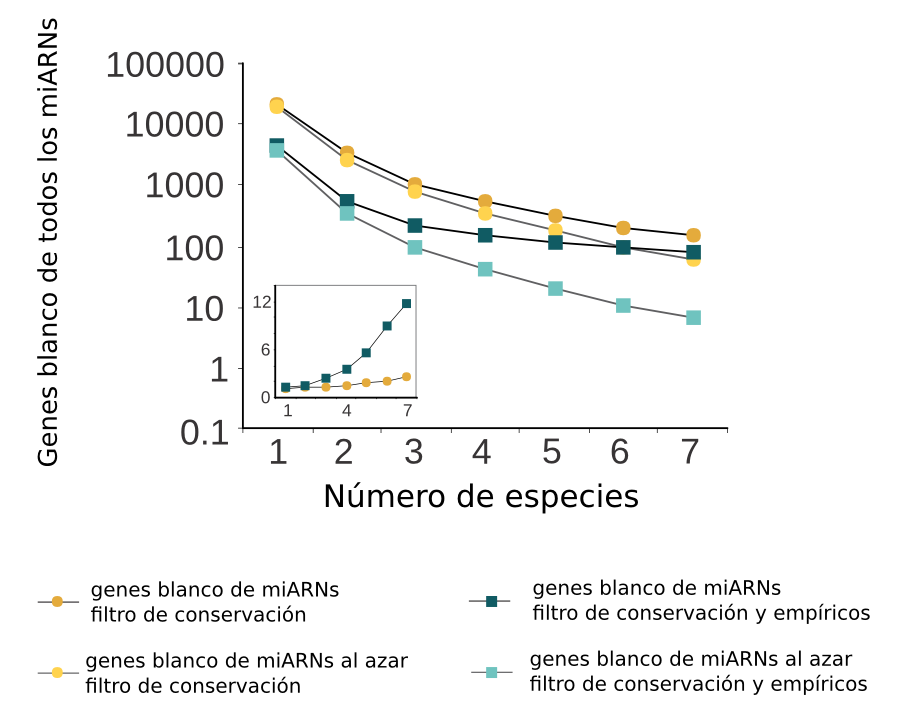
\includegraphics[width=0.5\textwidth]{img/NAR_fig2_05.png}
	\end{center}
\end{frame}

\begin{frame}{El número de genes blancos candidatos y la relación señal/ruido es variable entre los distintos miARNs}
	\begin{center}
		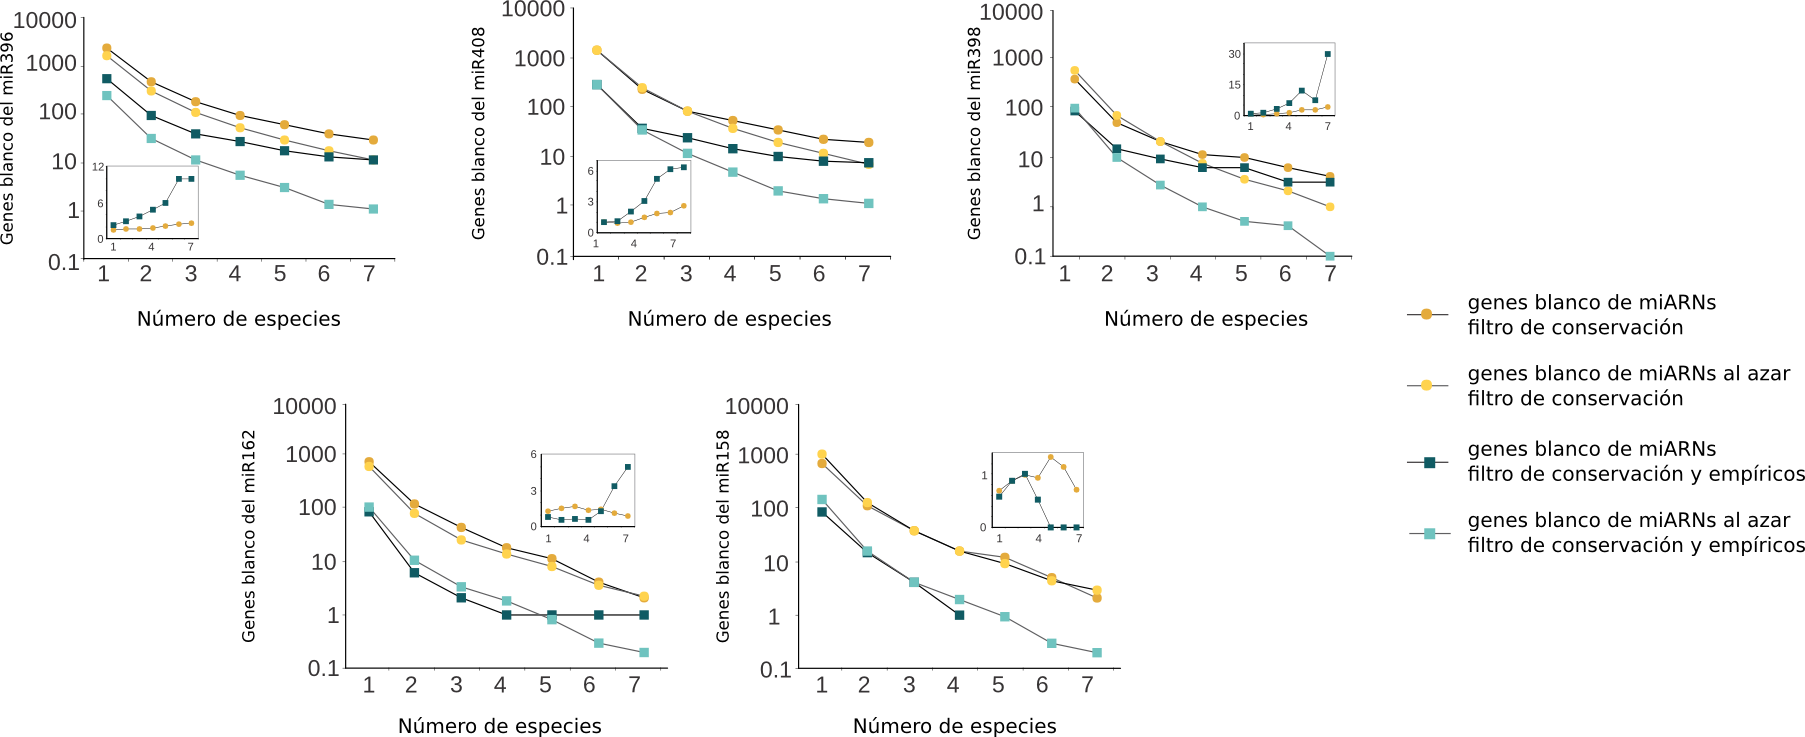
\includegraphics[width=1\textwidth]{img/NAR_fig2_bis.png}
	\end{center}
\end{frame}

\begin{frame}{Potenciales genes blancos utilizando solo conservación evolutiva}
	\begin{center}
		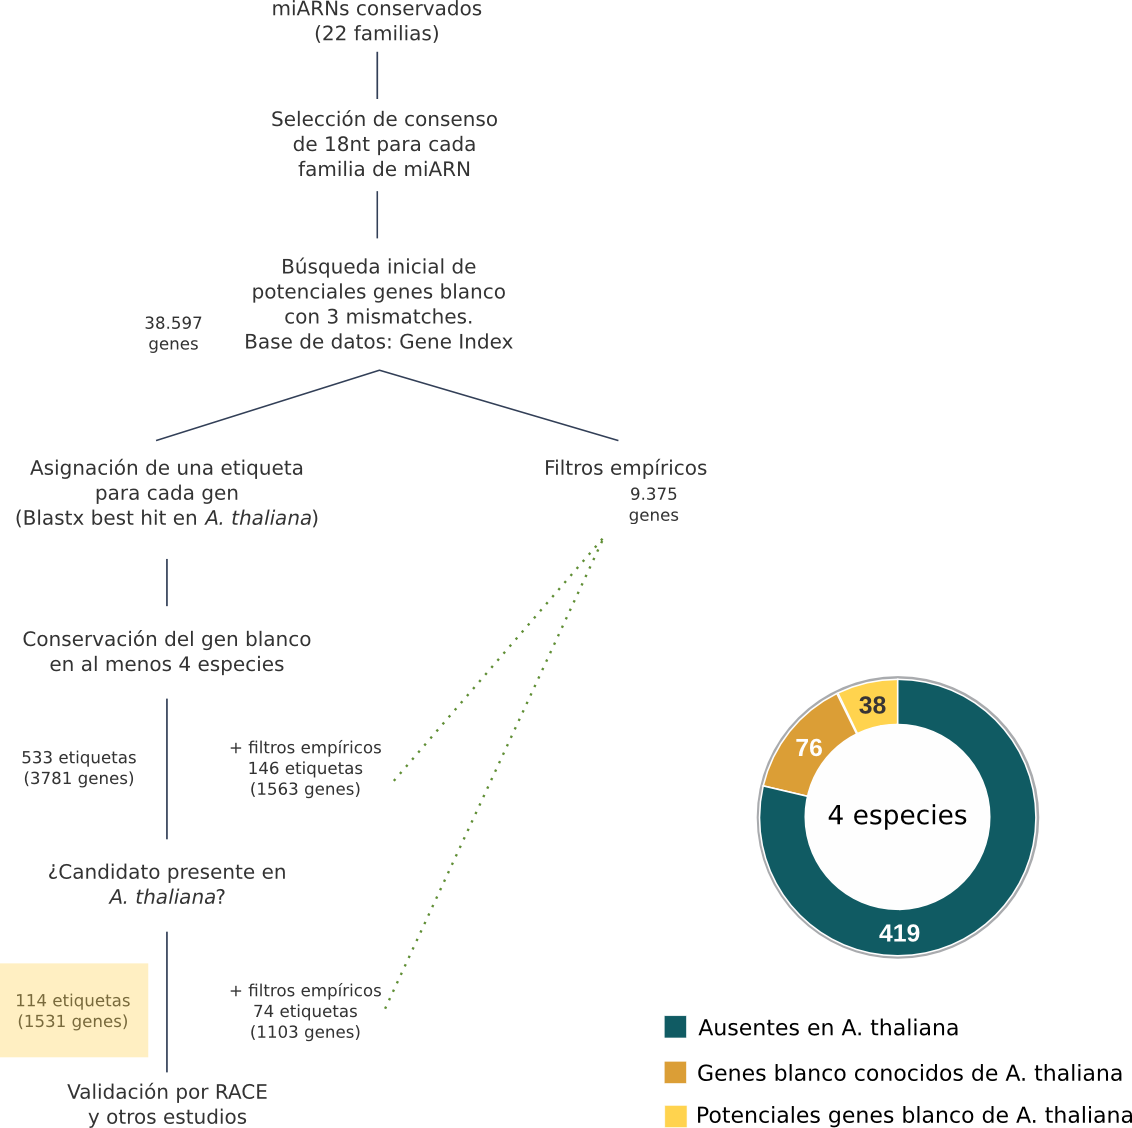
\includegraphics[width=.7\textwidth]{img/NAR_fig01y03.png}
	\end{center}
\end{frame}

\begin{frame}{Nuevos genes blancos validados en \textit{A. thaliana}}
	\begin{center}
		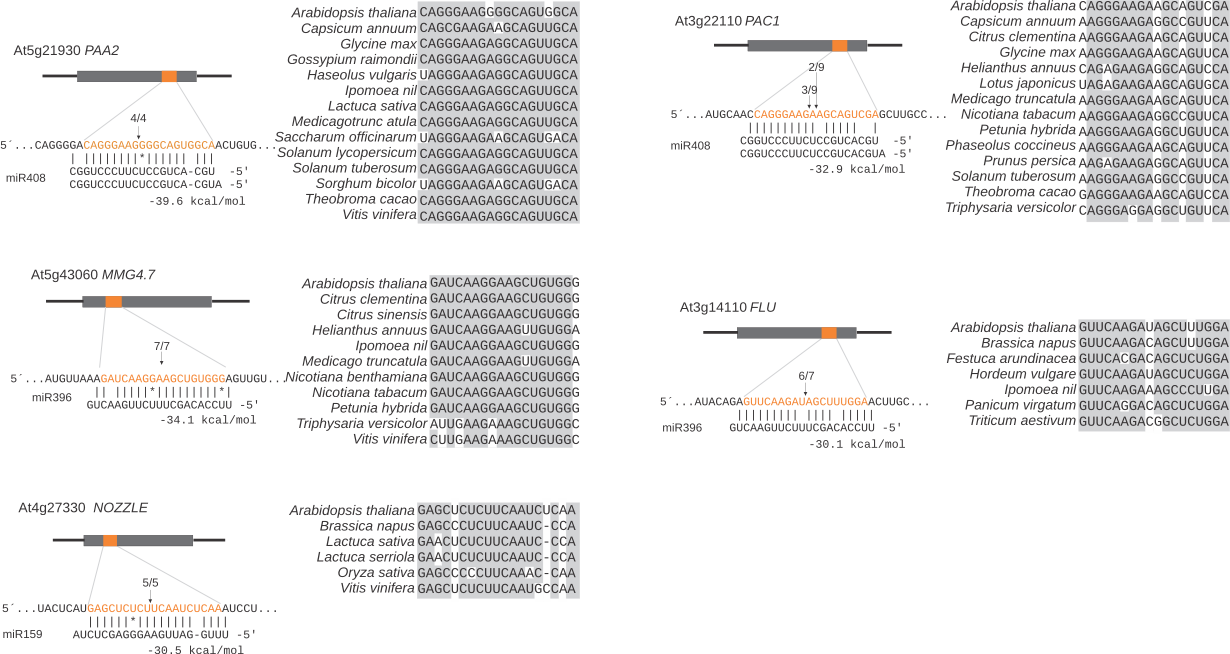
\includegraphics[width=1\textwidth]{img/Figure4_retocada.png}
	\end{center}
\end{frame}

\begin{frame}{Nuevos genes blancos con interacciones G-U}
	\begin{center}
		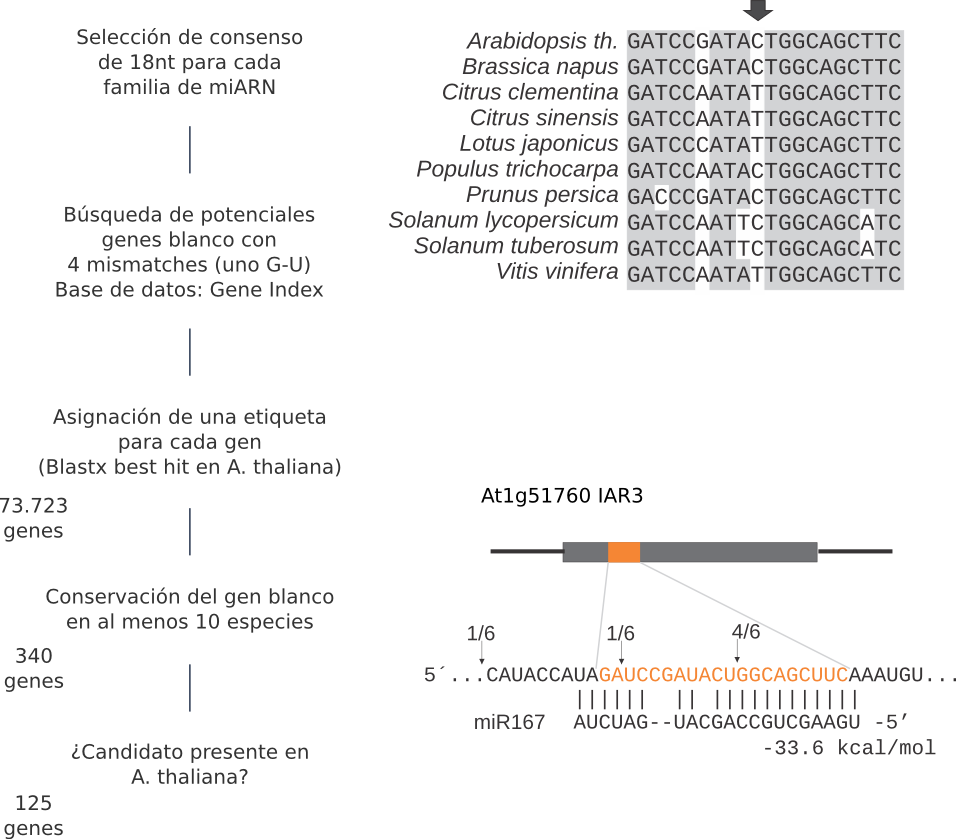
\includegraphics[width=.6\textwidth]{img/Figure5_retocada.png}
	\end{center}
\end{frame}

\begin{frame}{Identificación de genes blancos específicos de \textit{Solanaceae}}
	\begin{center}
		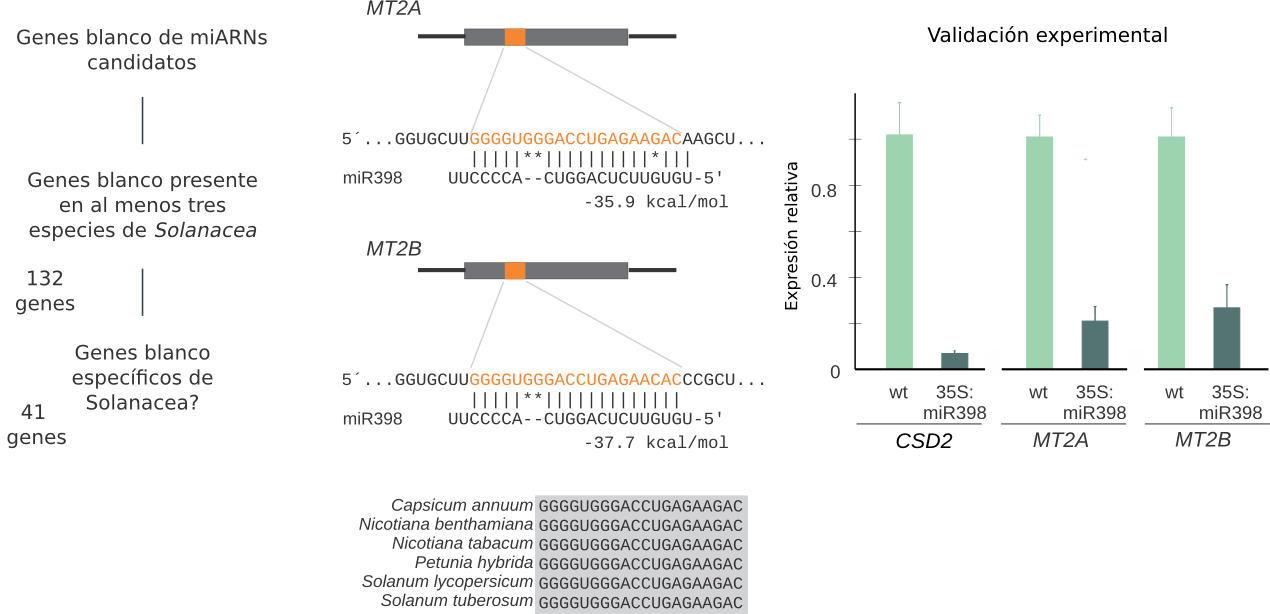
\includegraphics[width=.8\textwidth]{img/Figure6_retocada.png}
	\end{center}
\end{frame}


\begin{frame}{Herramienta para la predicción de genes blancos regulados por miARNs en plantas}
ComTAR, una herramienta para predecir potenciales genes blancos regulados por miARNs en plantas basada en la conservación evolutiva del par miARN-gen blanco. Permite realiza la búsqueda de:

%~ con un número relajado de ``mismatches''

\begin{itemize}
    \item potenciales genes blancos a partir de un miARN.
    \item familias de potenciales genes blancos de un miARN.
    \item un gen de interés para ver si es potencial gen blanco de algún miARN conservado
    \item nuevos ARNs pequeños
\end{itemize}
    \begin{center}
        \uncover<2->{\href{http://rnabiology.ibr-conicet.gov.ar/comtar}{\beamergotobutton{http://rnabiology.ibr-conicet.gov.ar/comtar}}}
    \end{center}
\end{frame}

\begin{frame}{Potenciales genes blancos del miR398}
	\begin{center}
		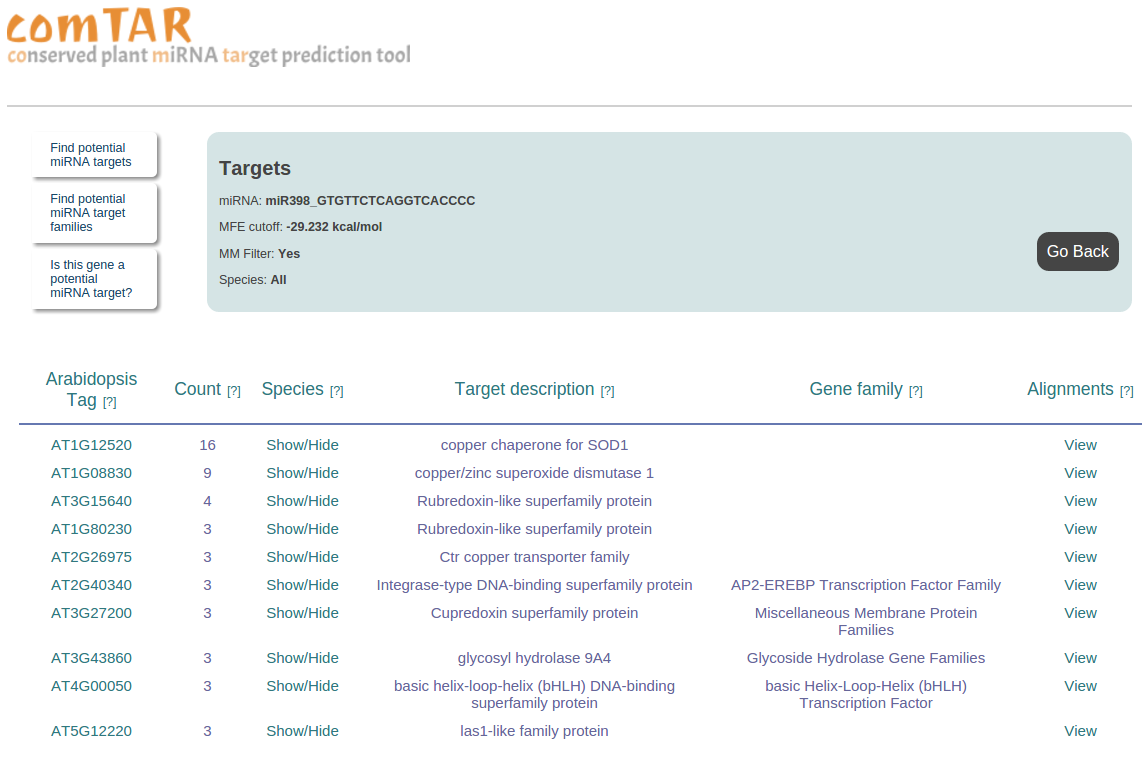
\includegraphics[width=.8\textwidth]{img/comTAR_find_targets.png}
	\end{center}
\end{frame}

\begin{frame}{ComTAR permite visualizar el alineamiento, energía de hibridación en cada especie}
	\begin{center}
		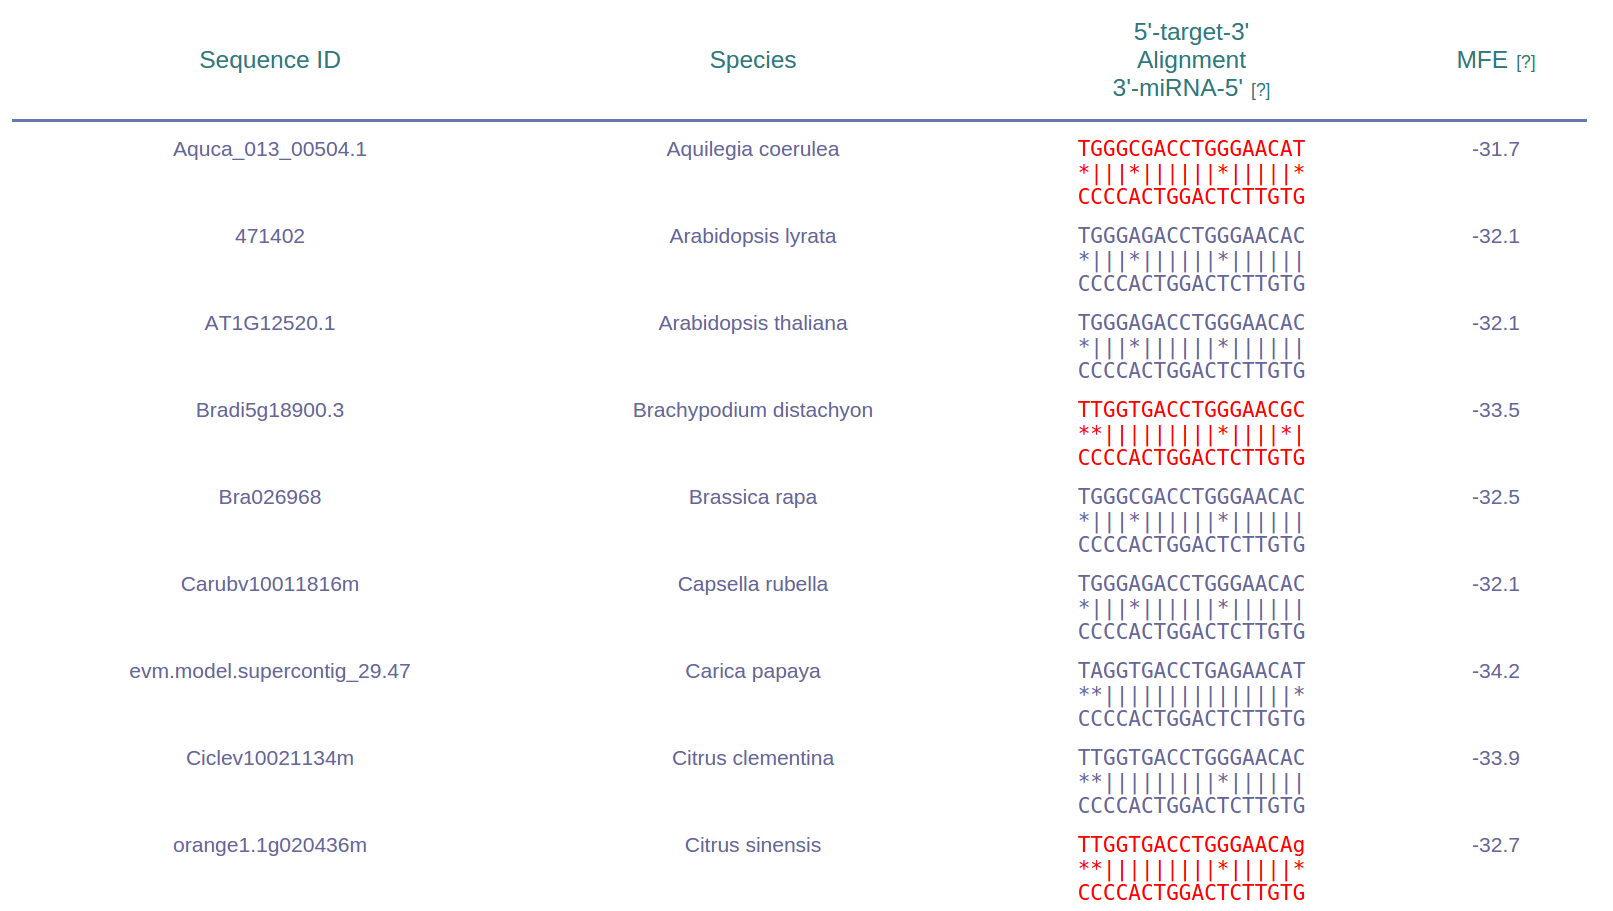
\includegraphics[width=.7\textwidth]{img/comTAR_fig2.png}
	\end{center}
\end{frame}


\begin{frame}{Conclusiones I}
	\begin{center}
		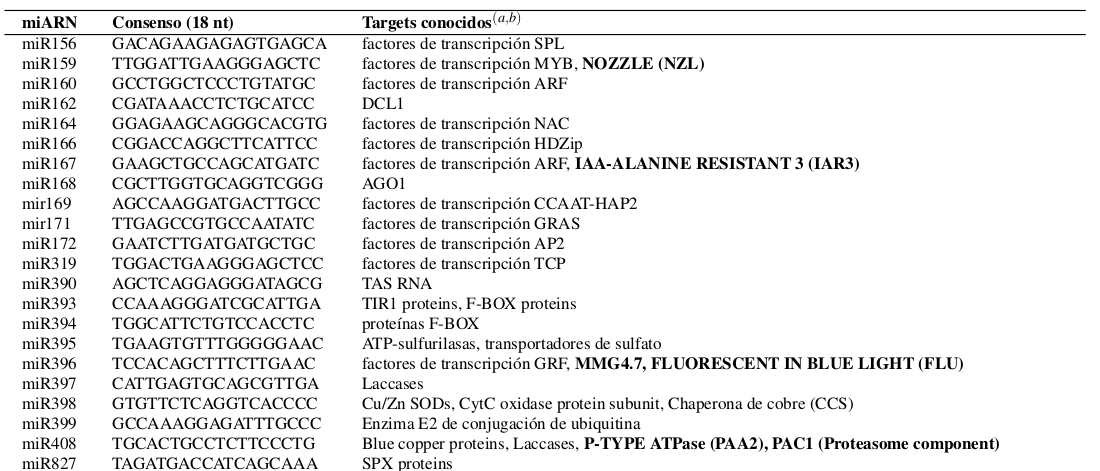
\includegraphics[width=.8\textwidth]{img/miRNAs_y_genes_blancos.png}
	\end{center}
\end{frame}

\begin{frame}{Conclusiones I}
	\begin{itemize}
        \item<1-> Diseñamos una estrategia para identificar genes blancos regulados por miARNs en plantas, basado en la conservación evolutiva del par miARN-gen blanco.
        \item<2-> Identificamos nuevos genes blancos en \textit{A. thaliana} y se validaron experimentalmente varios de ellos.
        %~ a pesar de que este sistema ya había sido estudiado en detalles en distintos enfoques genómicos. 
        \item<3-> Esta estrategia puede ser utilizada para identificar genes blancos presentes en un grupo específico de especies.
        \item<4-> Interacciones miARN-gen blanco conservadas probablemente participen en procesos biológicos relevantes
        \item<5-> Desarrollamos una herramienta web denominada comTAR para predecir potenciales genes blancos regulados por miARNs en plantas
	\end{itemize}
\end{frame}


\subsection{Resultados 2}

\begin{frame}{Objetivos específicos}
    \setbeamercovered{transparent=25}
		\pause
		\begin{itemize}
            \item<-1> Diseñar una estrategia y una herramienta web para la identificación de genes blancos regulados por miARNs en plantas.
			\item<-2> Desarrollar herramientas para el análisis de los intermediarios de procesamiento de miARNs en plantas.
			\item<-2> Identificar y caracterizar precursores de miARNs en distintas especies que tengan mecanismos de procesamiento distintos.
			\item<-1> Caracterizar la relación entre la evolución de los precursores de miARNs en plantas y los mecanismos de procesamiento determinados previamente.
        \end{itemize}
\end{frame}

%~ Estudios genómicos sobre la biogénesis de precursores de miARNs en plantas.

\begin{frame}{Precursores en plantas son muy variables en tamaño y forma}
	\begin{center}
		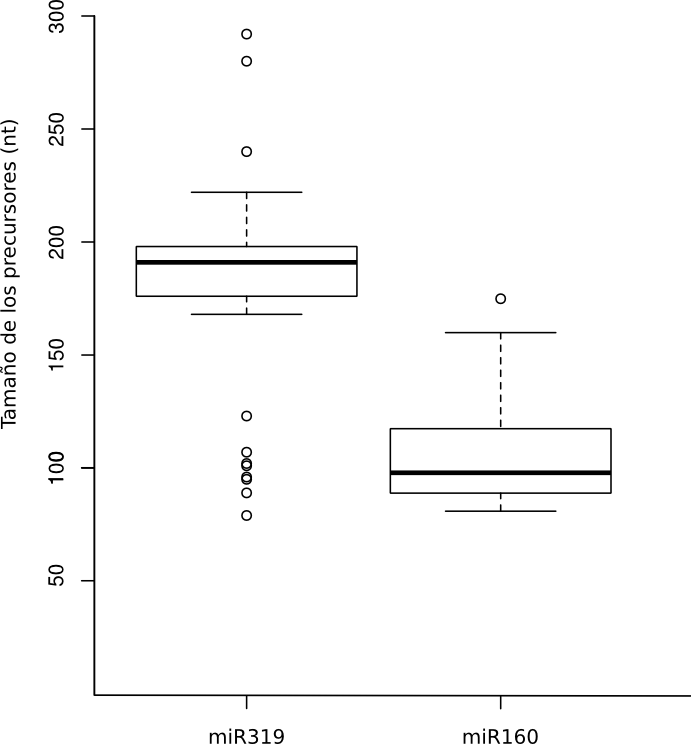
\includegraphics[width=.5\textwidth]{img/hairpin_distribution.png}
	\end{center}
\end{frame}

\begin{frame}{Bibliotecas SPARE para estudios genómicos de biogénesis de miARNs en plantas}
\begin{columns}
    \begin{column}{0.3\textwidth}
		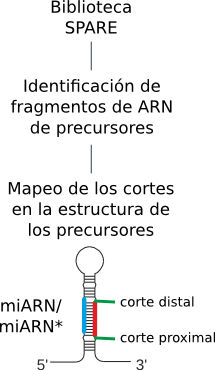
\includegraphics[width=.6\textwidth]{img/GR_fig1C.png}
    \end{column}
    \begin{column}{0.7\textwidth}
        \uncover<2->{
            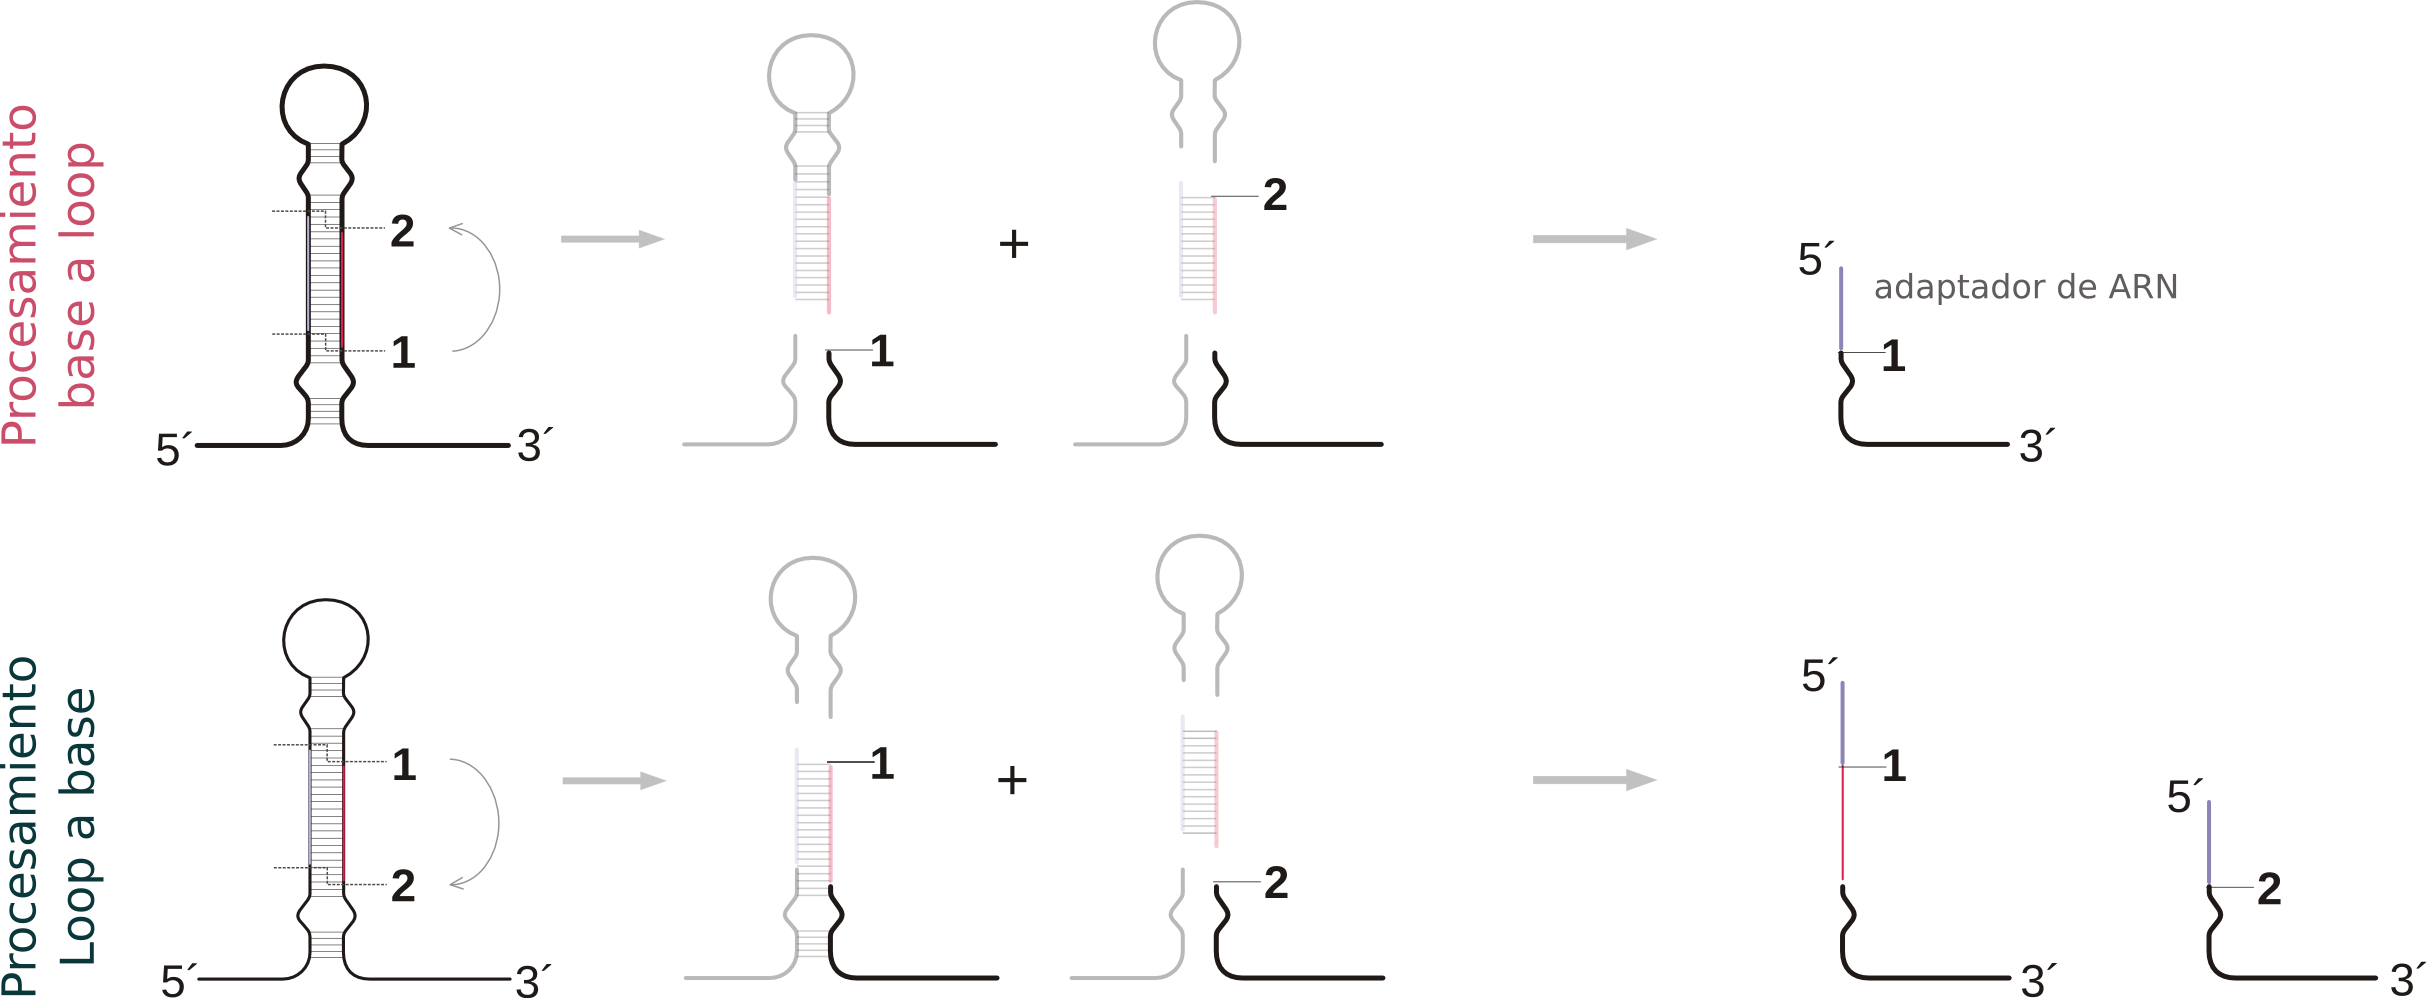
\includegraphics[width=1\textwidth]{img/SPARE_tecnica.png}
        }
    \end{column}
\end{columns}
\end{frame}


\begin{frame}{Visualización de precursores que se procesan desde la base}
	\begin{center}
		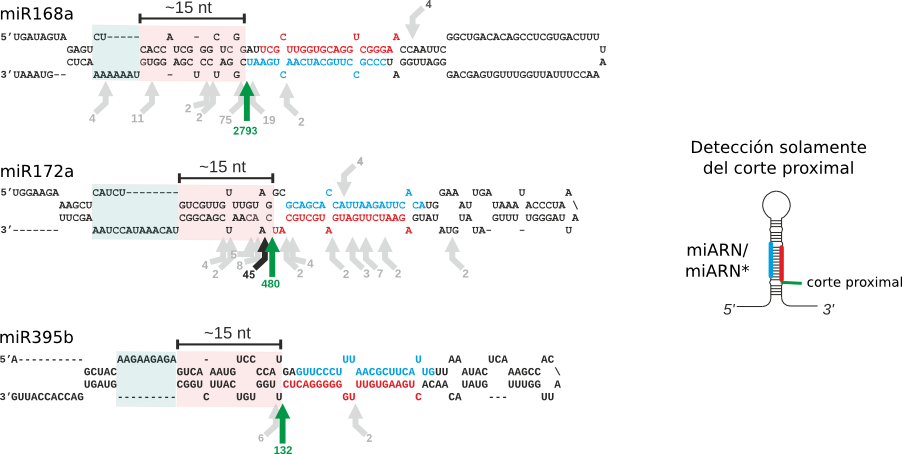
\includegraphics[width=.8\textwidth]{img/GR_fig2A.png}
	\end{center}
\end{frame}

\begin{frame}{Visualización de precursores que se procesan desde el loop}
	\begin{center}
		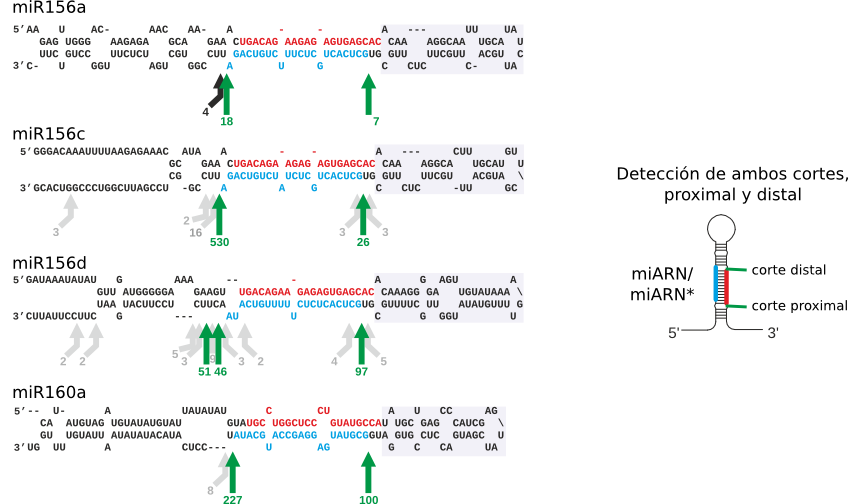
\includegraphics[width=.8\textwidth]{img/GR_fig4A.png}
	\end{center}
\end{frame}



\begin{frame}{Bibliotecas de SPARE}
\begin{table}[]
    \centering
    \tiny
    \begin{tabular}{llccc}
        \multicolumn{1}{c}{\textbf{Bibliotecas}} & \multicolumn{1}{c}{\textbf{Muestras}} &  \textbf{\begin{tabular}[c]{@{}c@{}}Secuencias\\ totales \\\end{tabular}} &  \textbf{\begin{tabular}[c]{@{}c@{}}Secuencias\\ que mapean\\ los precursores\end{tabular}} &  \textbf{\begin{tabular}[c]{@{}c@{}}Secuencias únicas\\ que mapean\\ los precursores\end{tabular}} \\
        col\_2AB                                 & Col-0 réplica 1. Control de fiery y hyl1 & 13911694                                                                 & 80166                                                                                      & 308                                                                                               \\
        col\_3AB                                 & Col-0 réplica 2. Control de fiery y hyl1 & 16618008                                                                 & 126556                                                                                     & 426                                                                                               \\
        Col\_AD                                  & Col-0 réplica 1. Control de se           & 13758567                                                                 & 119368                                                                                     & 496                                                                                               \\
        Col\_BC                                  & Col-0 réplica 2. Control de se           & 14648459                                                                 & 241973                                                                                     & 553                                                                                               \\
        FIERY\_1AB                               & fiery réplica 1                          & 9832923                                                                  & 470789                                                                                     & 1655                                                                                              \\
        FIERY\_4                                 & fiery réplica 2                          & 23529725                                                                 & 821562                                                                                     & 1752                                                                                              \\
        HYL\_1                                   & hyl1 réplica 1                           & 10171629                                                                 & 45653                                                                                      & 316                                                                                               \\
        HYL\_2                                   & hyl1 réplica 2                           & 8864406                                                                  & 35860                                                                                      & 320                                                                                               \\
        SE\_BD                                   & se réplica 1                             & 15291993                                                                 & 299513                                                                                     & 639                                                                                               \\
        SE\_CE                                   & se réplica 1                             & 25296809                                                                 & 510438                                                                                     & 693                                                                                              
    \end{tabular}
\end{table}
\end{frame}


\begin{frame}{Precursores procesados desde la base}
	\begin{center}
		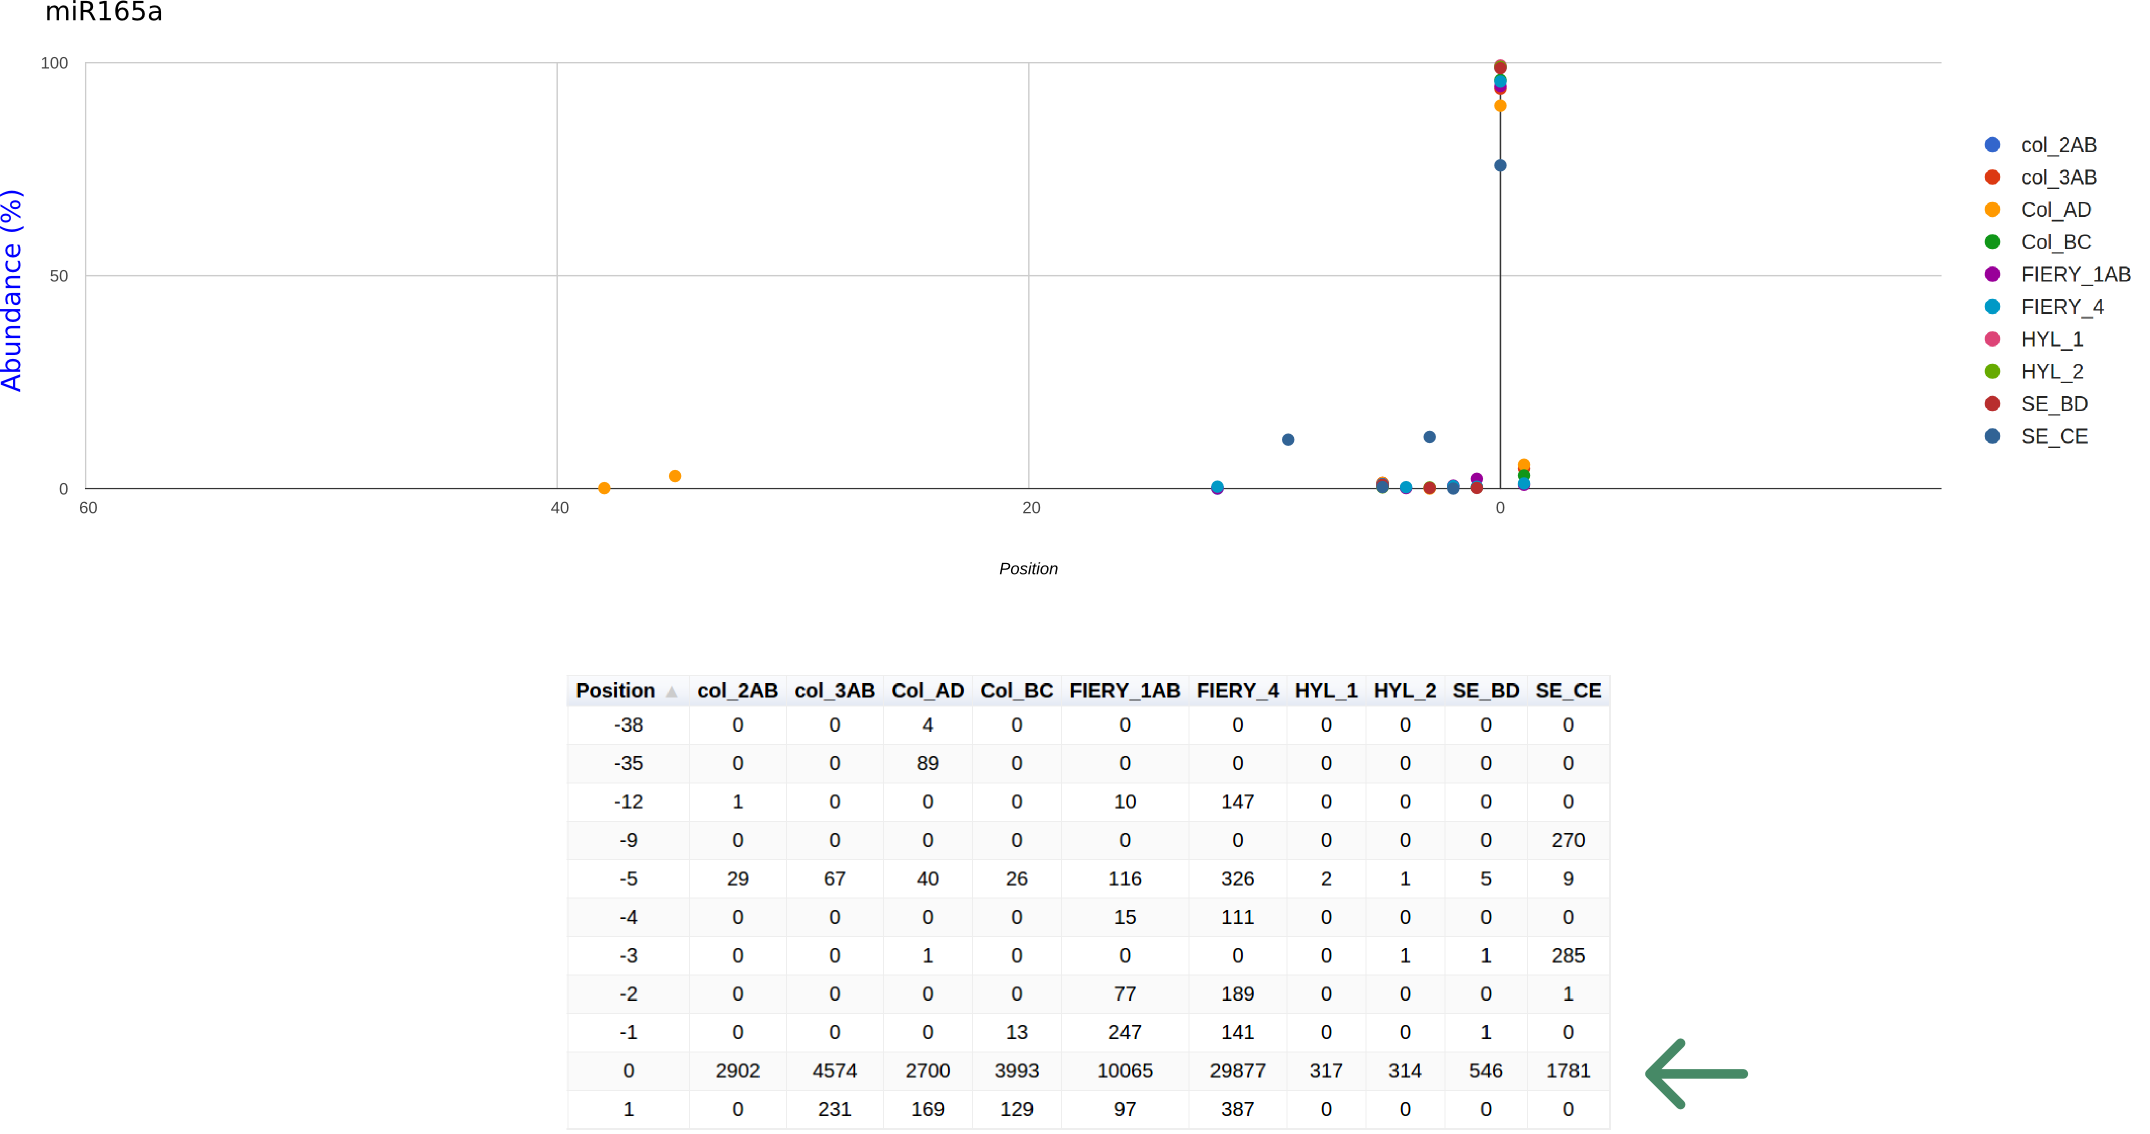
\includegraphics[width=1\textwidth]{img/miR165a_SPARE.png}
	\end{center}
\end{frame}

\begin{frame}{Precursores procesados desde el loop}
	\begin{center}
		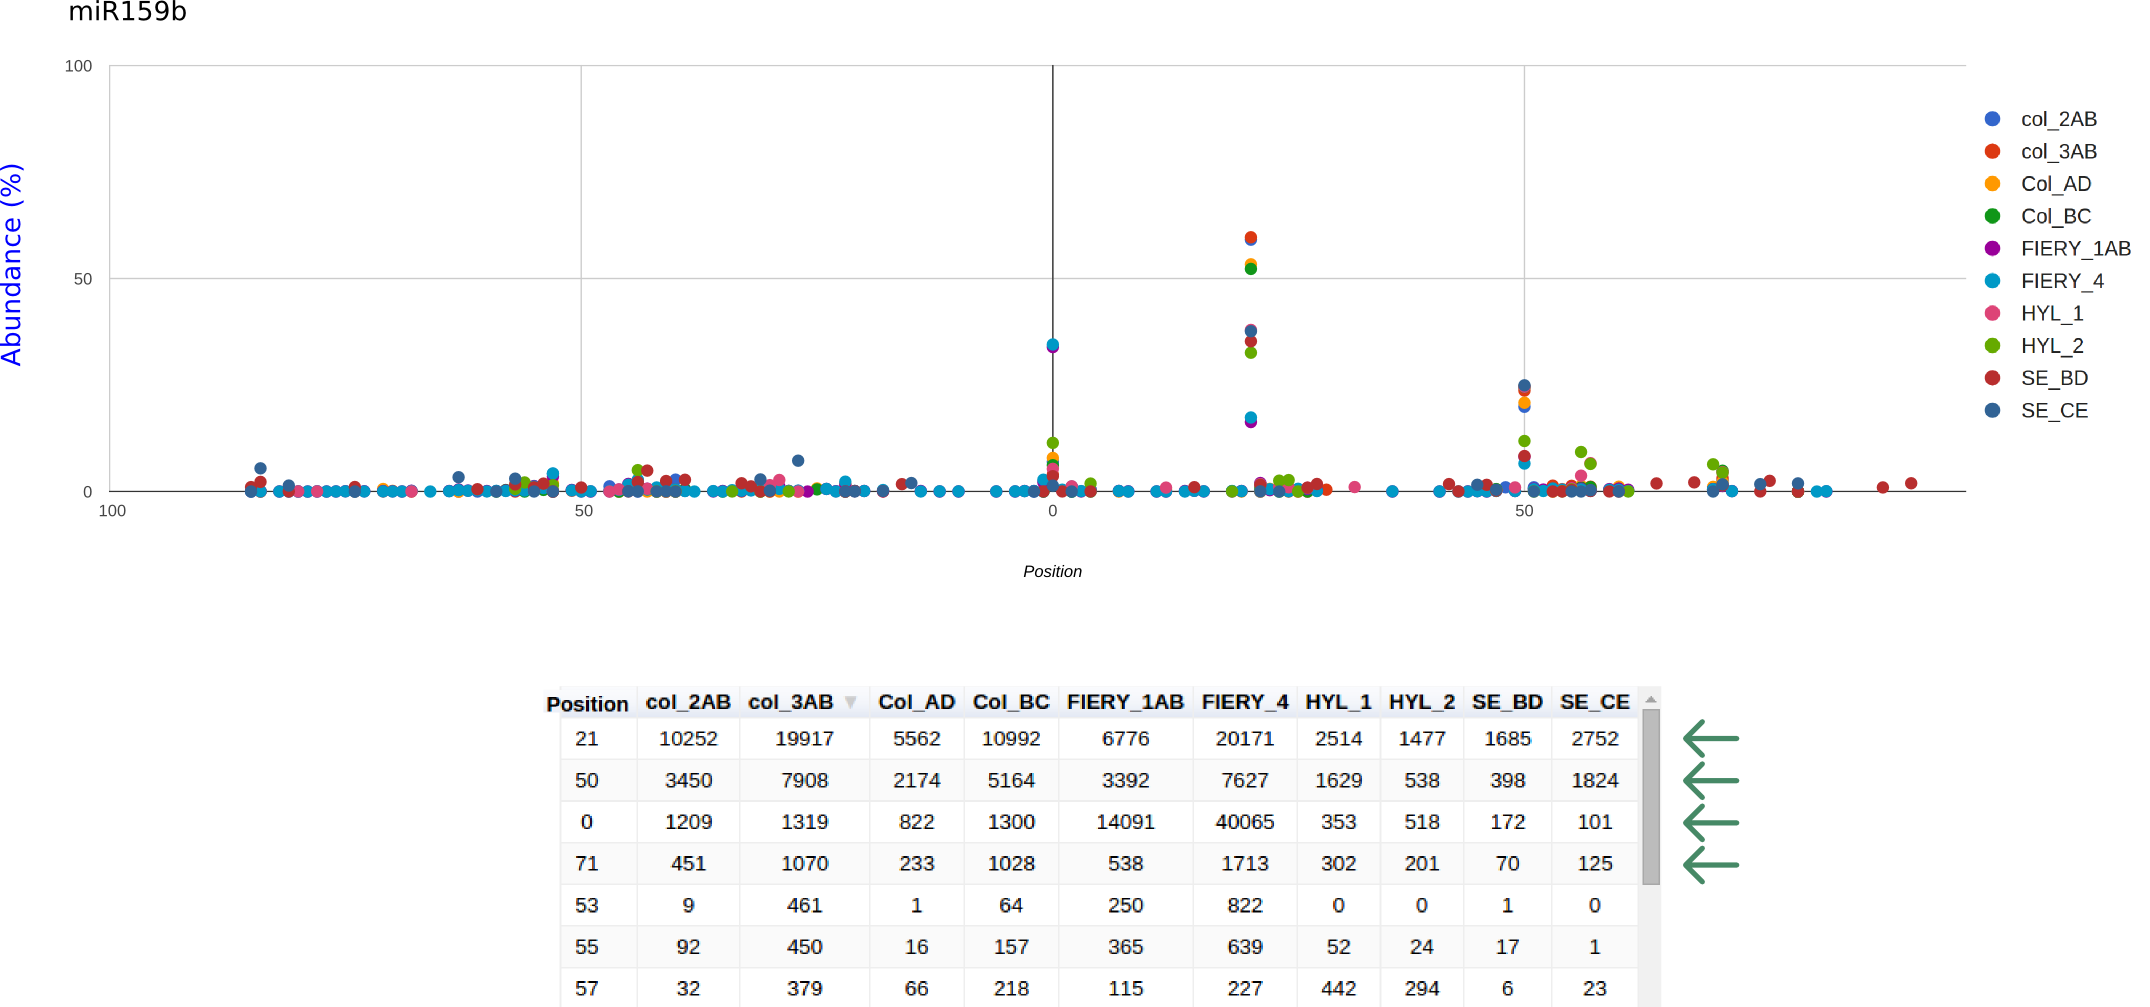
\includegraphics[width=1\textwidth]{img/miR159b_SPARE.png}
	\end{center}
\end{frame}

\begin{frame}{Tallo inferior de 15 nt en precursores procesados desde la base}
	\begin{center}
		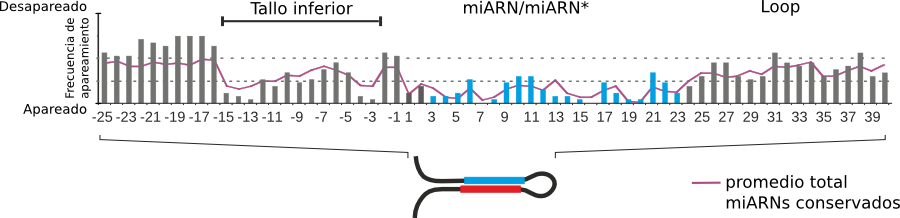
\includegraphics[width=.8\textwidth]{img/GR_fig2C.png}
	\end{center}
\end{frame}

\begin{frame}{Región terminal estructurada en precursores procesados desde el loop}
	\begin{center}
		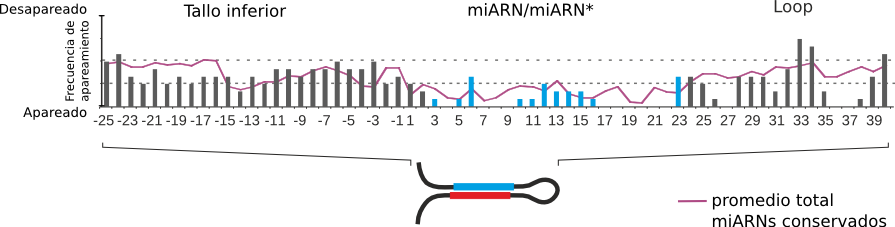
\includegraphics[width=.8\textwidth]{img/GR_fig4C.png}
	\end{center}
\end{frame}

\begin{frame}{Conclusiones II}
	\begin{center}
		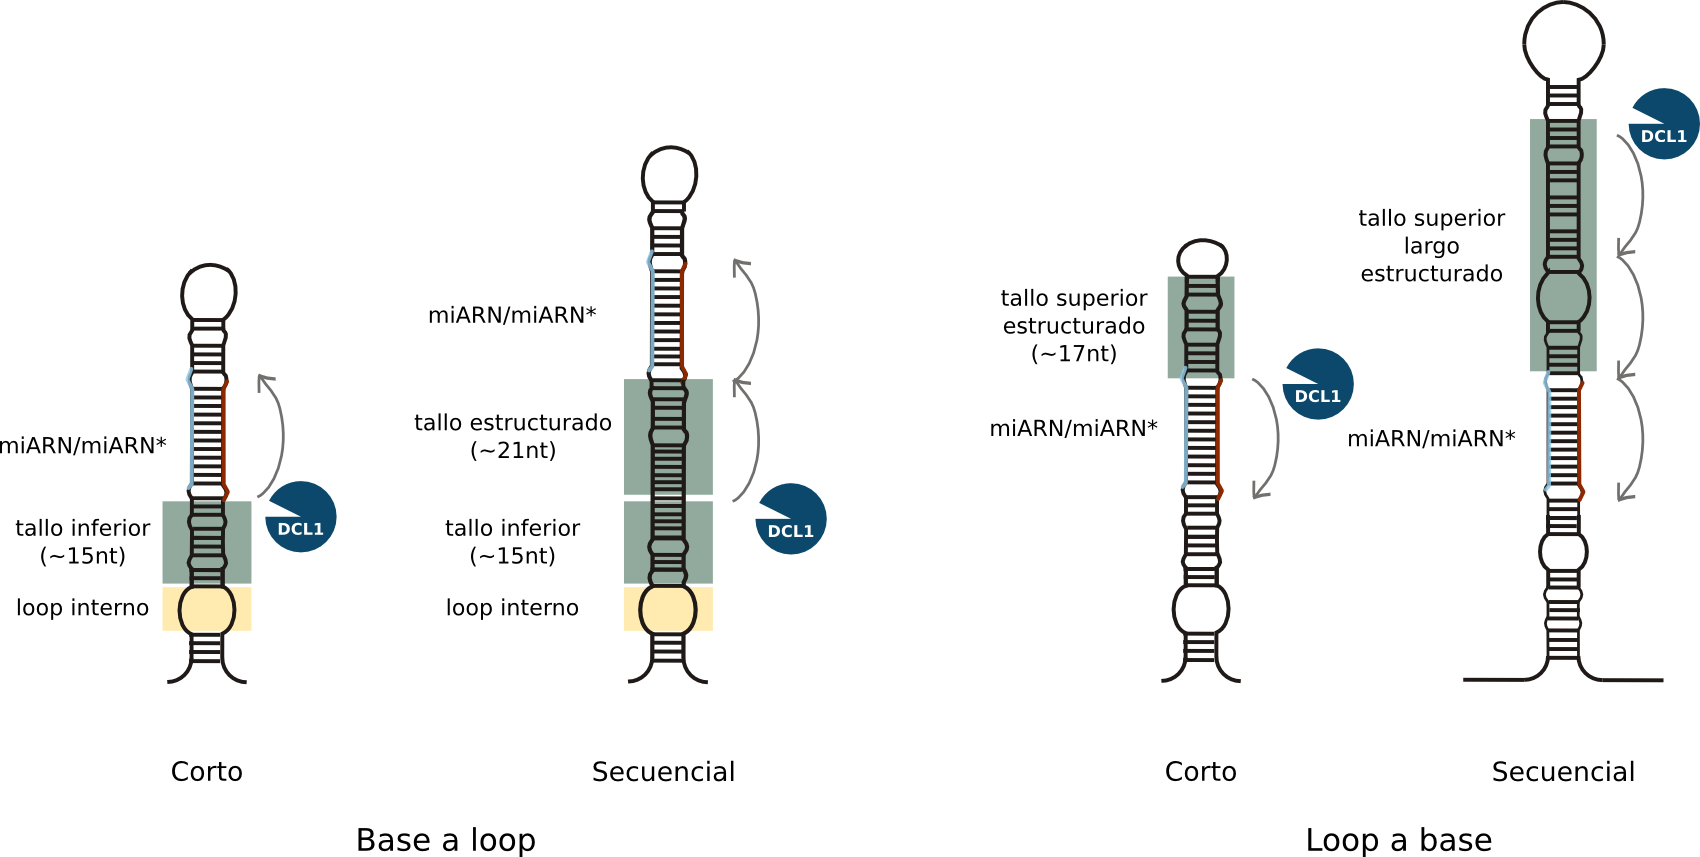
\includegraphics[width=1\textwidth]{img/mecanismos.png}
	\end{center}
\end{frame}


\begin{frame}{Búsqueda de ortólogos de precursores de miARNs.}
	\begin{center}
		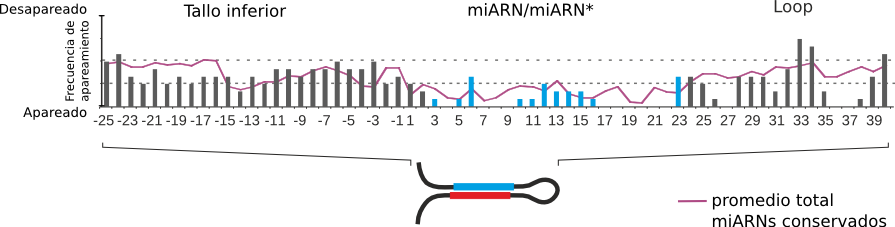
\includegraphics[width=.8\textwidth]{img/GR_fig4C.png}
	\end{center}
\end{frame}


%~ \begin{frame}{Conclusiones II}
%~ \begin{itemize}
    %~ \item En los precursores con un mecanismo \textbf{corto de base a loop}, un loop interno seguido por un tallo inferior de $\sim$15nt especifica la posición del primer corte.
        %~ Esta estructura se encuentra en la mayoría de familias de miARNs.
        %~ A pesar de que el tallo puede contener bulges, la transición de un loop interno (simple hebra) al tallo inferior es bastante marcada, y tres pares de bases apareadas generalmente definen el comienzo del tallo inferior del precursor.
        %~ El segundo corte procede a una distancia fija de $\sim$21 nt desde la posición del primer corte.
    %~ \item En los precursores con un mecanismo \textbf{secuencial de base a loop} (ej: familia del miR169), el primer corte procede como en los cortos de base a loop, pero luego son necesario dos cortes más para liberar el miARN, generando en el proceso niveles bajos de RNA pequeños adicionales.
    %~ \item En los precursores con un mecanismo \textbf{cortos de loop a base} (ej: familia del miR156 y miR160), el procesamiento es guiado por un tallo superior, y son necesarios dos cortes para liberar el miARN maduro.
        %~ La región terminal de estos precursores tienen una largo conservado de $\sim$42 donde incluye un loop pequeñ.
    %~ \item En los precursores con un mecanismo \textbf{secuencial de loop a base} (ej: familia del miR319 y miR159), cuatro cortes secuenciales por DCL1 son los encargados de procesar los precursores de miARNs.
        %~ En general muestran un tallo largo superior, del cual otros ARNs pequeños son generados.
%~ \end{itemize}
%~ \end{frame}

\subsection{Resultados 3}

\begin{frame}{Objetivos específicos}
    \setbeamercovered{transparent=25}
		\pause
		\begin{itemize}
            \item<-1> Diseñar una estrategia y una herramienta web para la identificación de genes blancos regulados por miARNs en plantas.
			\item<-1> Desarrollar herramientas para el análisis de los intermediarios de procesamiento de miARNs en plantas.
			\item<-1> Identificar y caracterizar precursores de miARNs en distintas especies que tengan mecanismos de procesamiento distintos.
			\item<-2> Caracterizar la relación entre la evolución de los precursores de miARNs en plantas y los mecanismos de procesamiento determinados previamente.
        \end{itemize}
\end{frame}



\begin{frame}{Estrategia bioinformática para el estudio de la evolución y biogénesis de miARNs en plantas}
VER LO QUE PUSE EN EL SEMINARIO IBR!!!!!

    Comenzamos nuestro análisis con una definición arbitraria de los precursores de plantas incluyendo 150 nt fuera del par miARN/miARN*.
    Para cada miembro de cada familia de A. thaliana no es trivial asignarle un ortólogo en otra especie teniendo en cuenta la anotación de miRBase. 
    Por esto, realizamos una búsqueda de ortólogos para cada miembro de cada familia de \textit{A. thaliana} utilizando como criterio la técnica de Blast recíproco.
\end{frame}


\begin{frame}{Existe un patrón estructural que comparten los precursores, en la región inmediata por debajo del dúplex miARN/miARN*}
	\begin{center}
		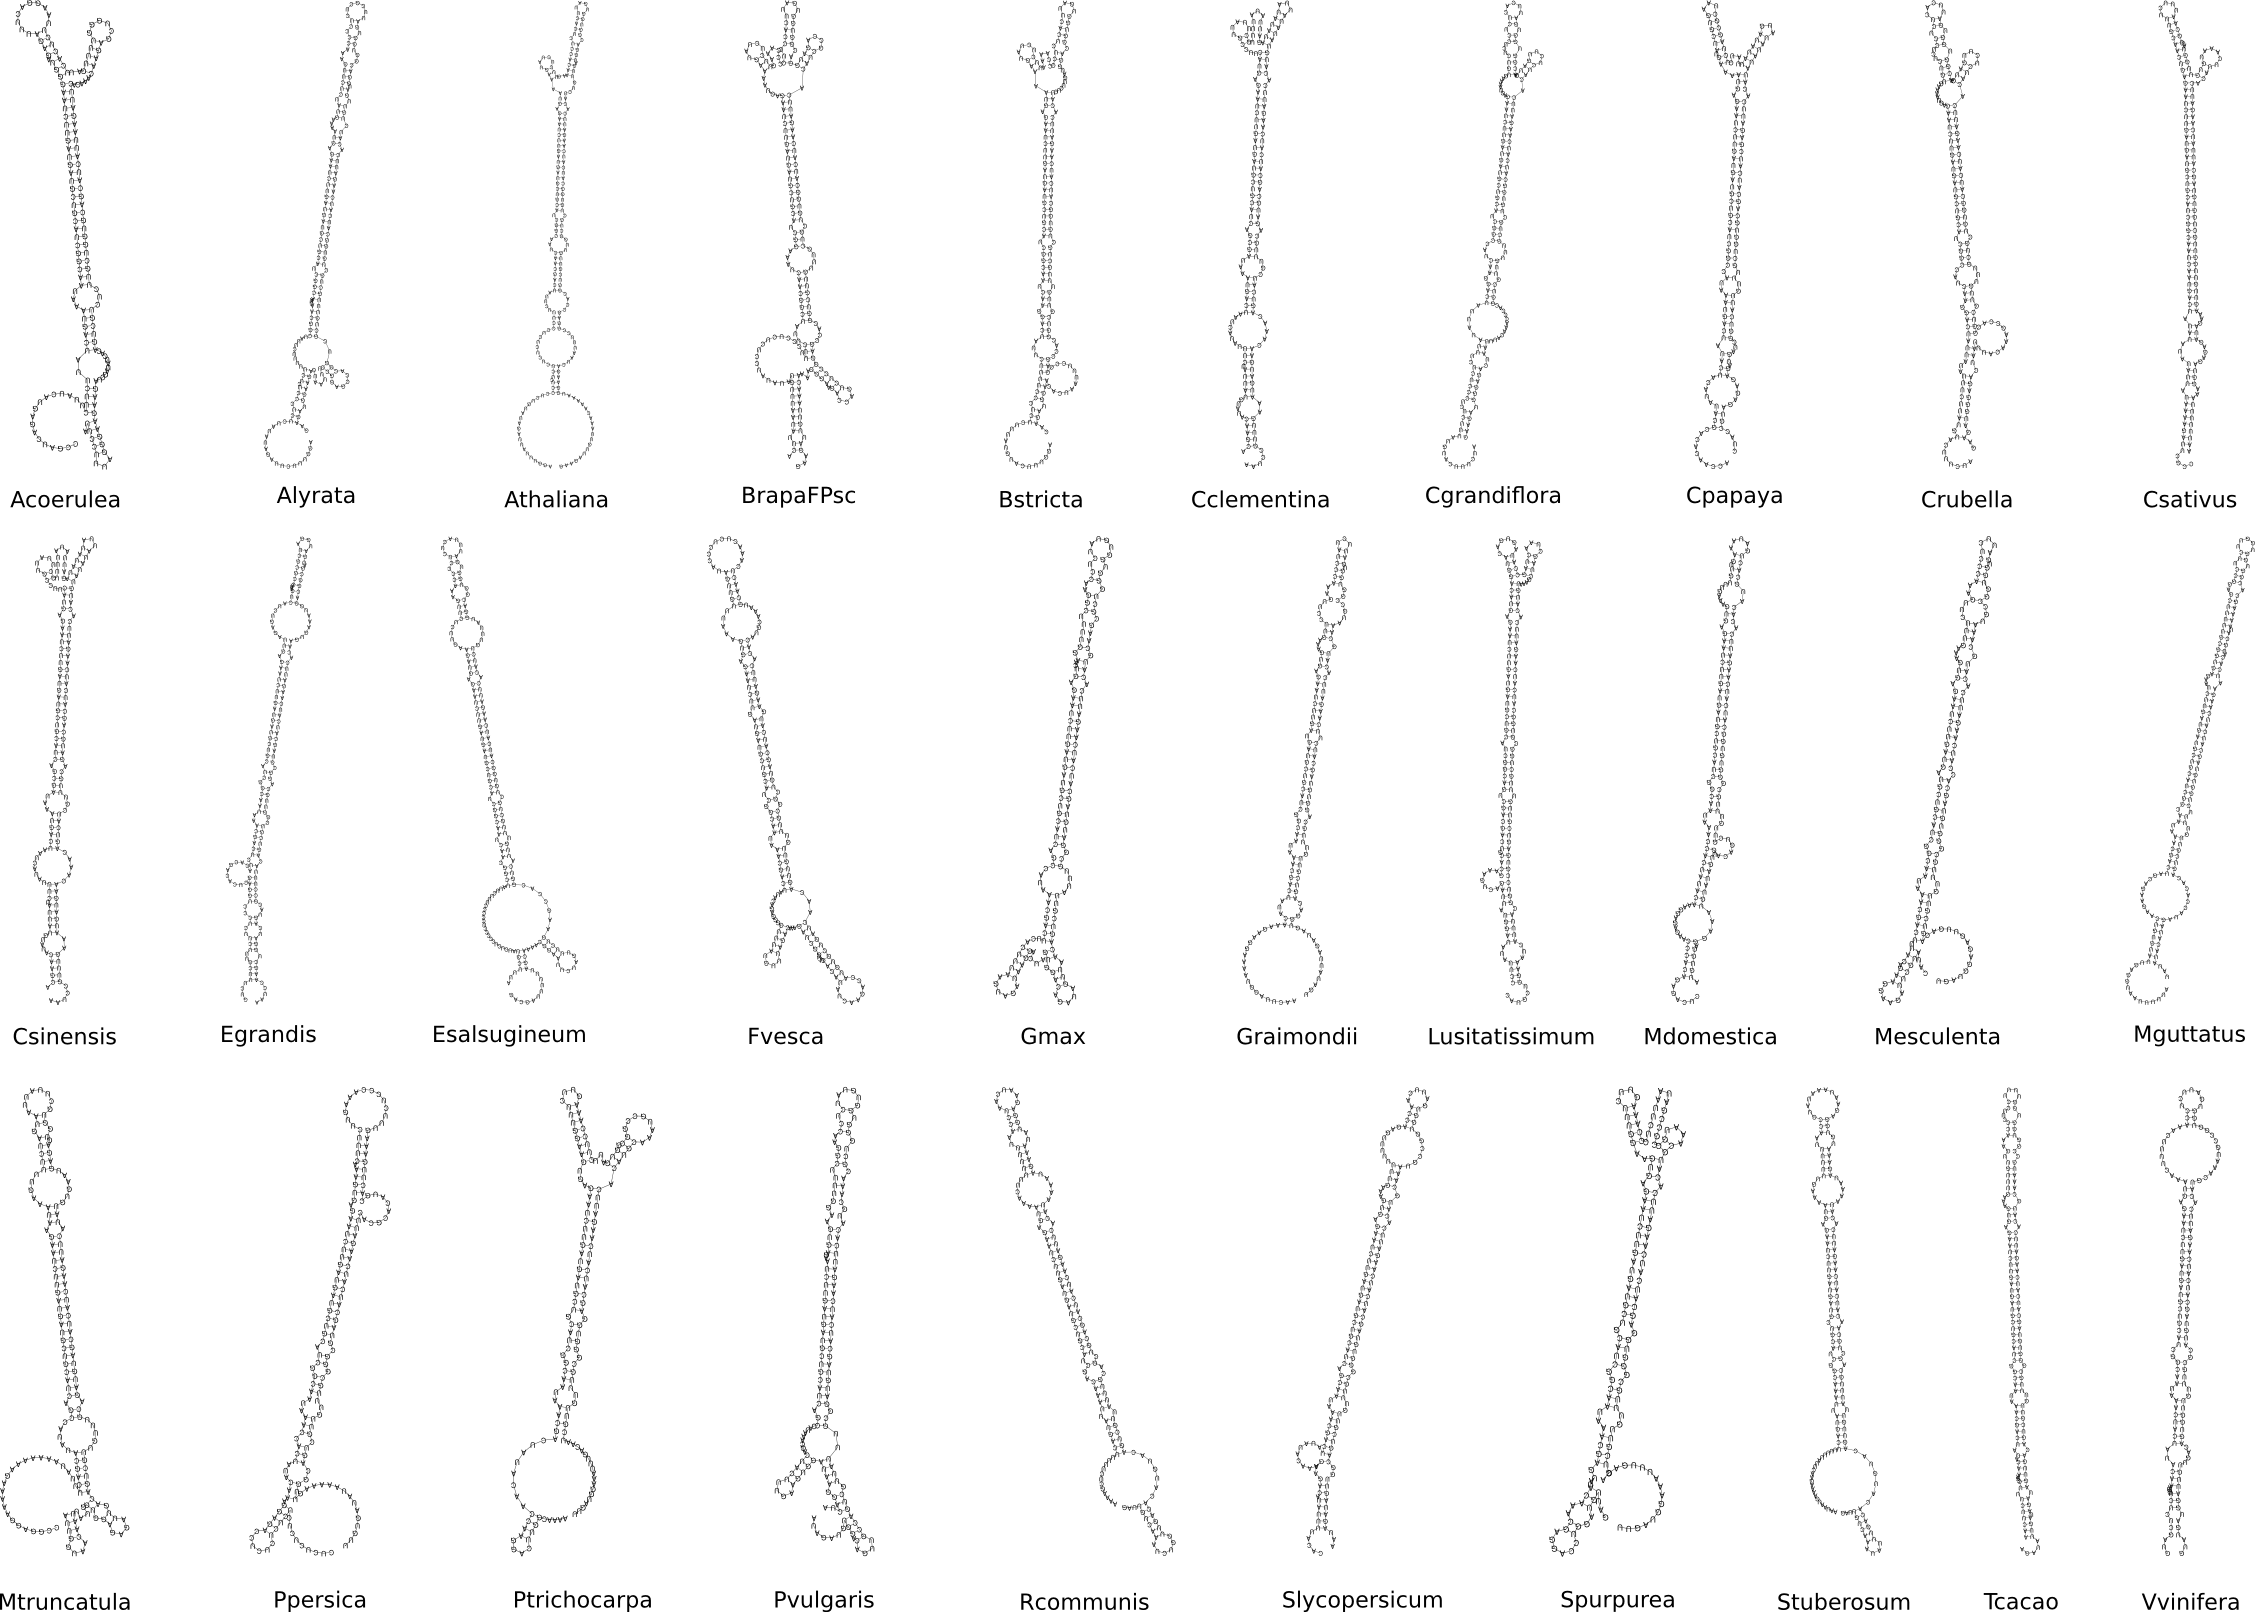
\includegraphics[width=.9\textwidth]{img/miR172a_rnafold.png}
	\end{center}
    \uncover<2->{Es difícil deducir información concreta a partir de esta figura.}
\end{frame}


\begin{frame}{Conservación de la secuencia primaria del miR172a en distintas especies}
	\begin{center}
		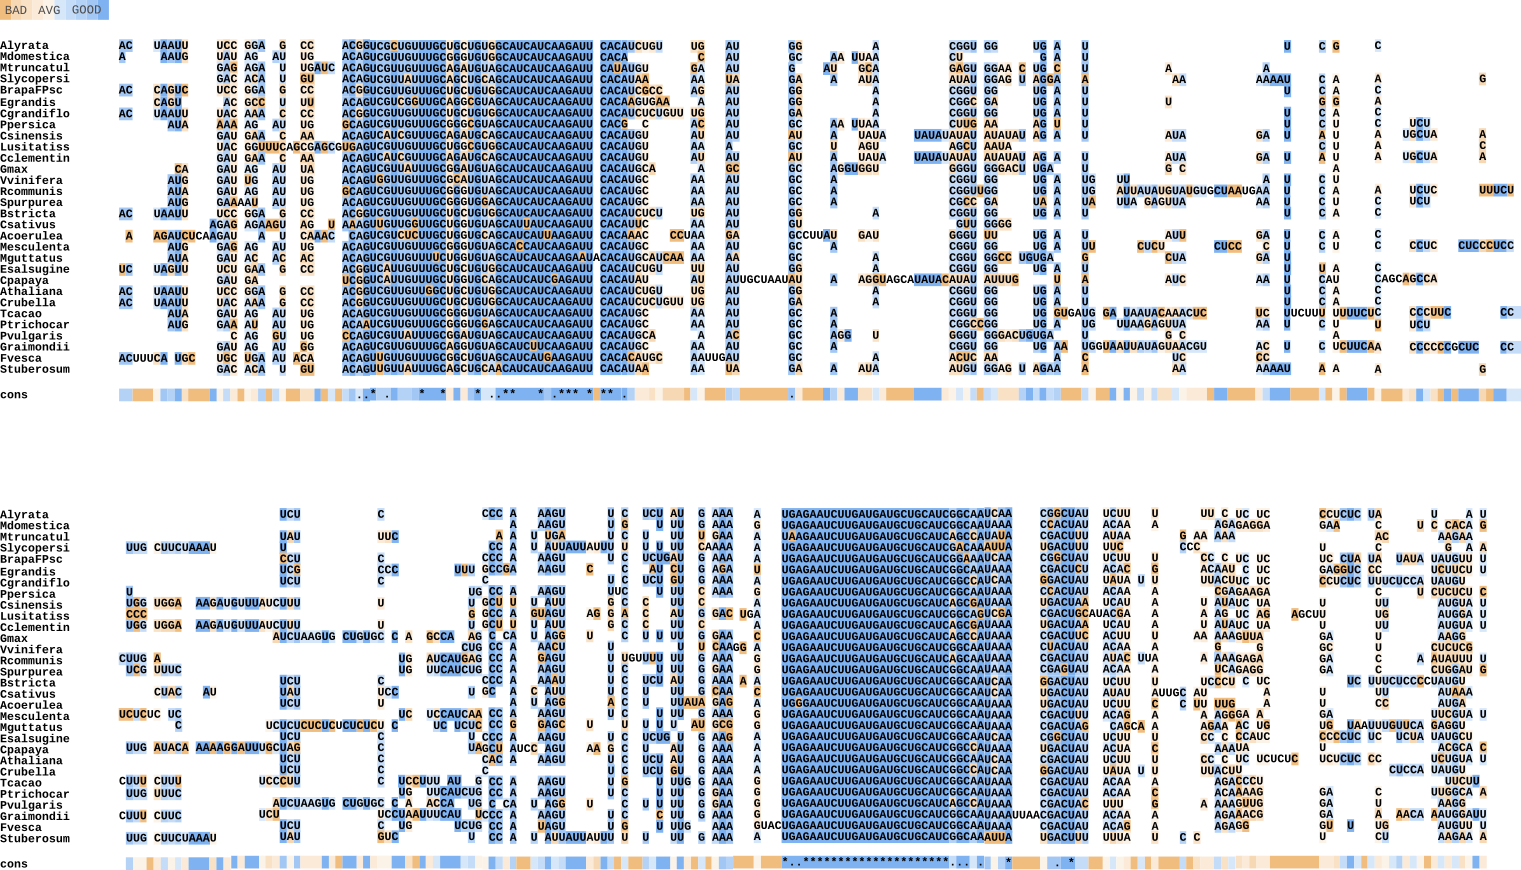
\includegraphics[width=1\textwidth]{img/miR172a_tcoffee_01.png}
	\end{center}
\end{frame}

\begin{frame}{El miR172a maduro y el miR172a* están conservados en las distintas especies}
	\begin{center}
		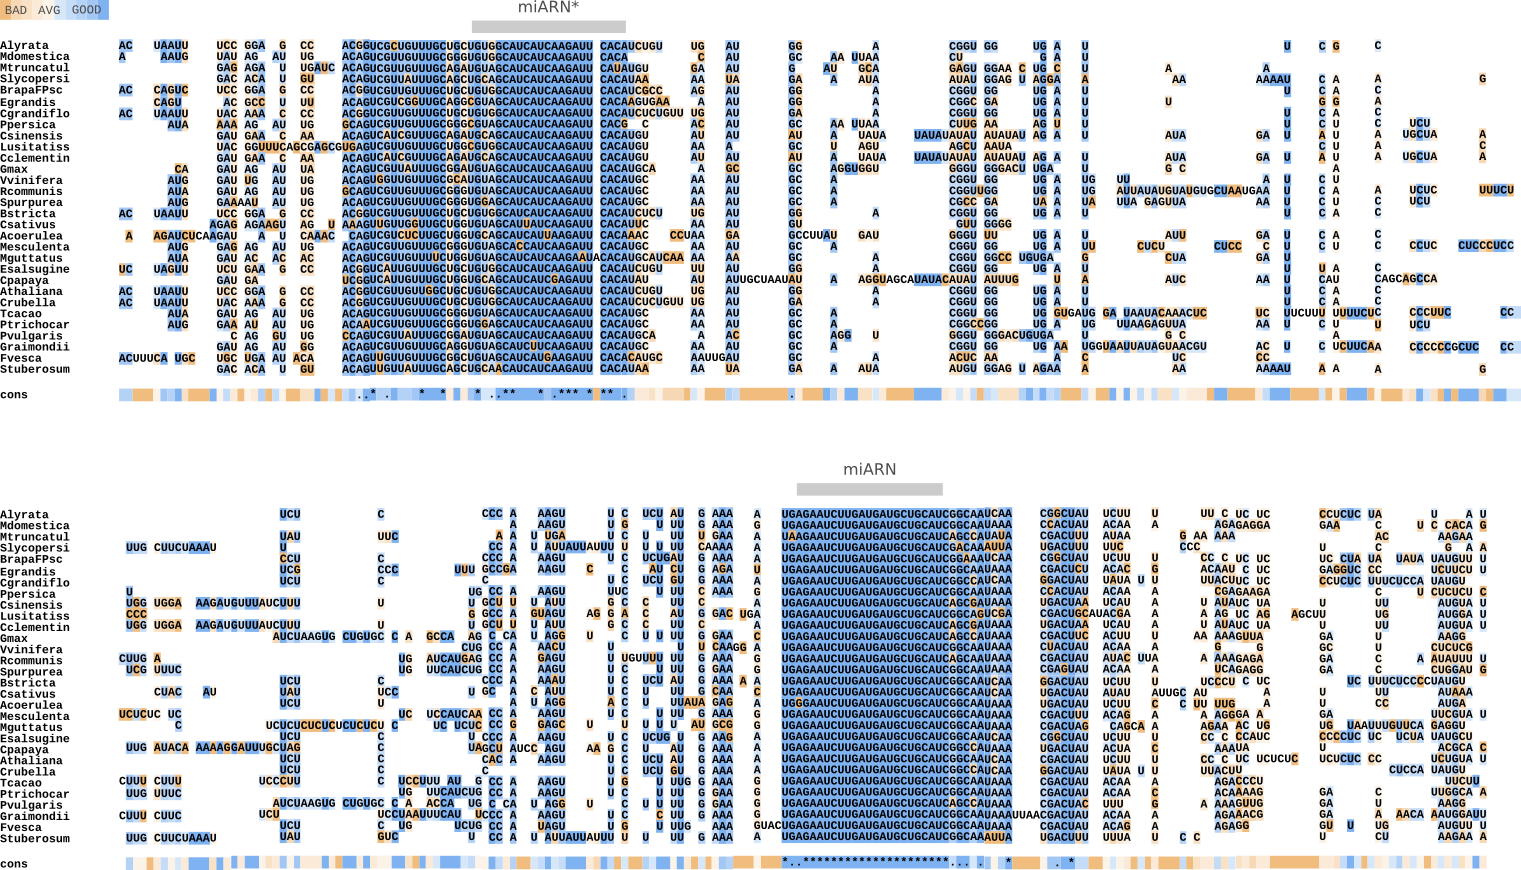
\includegraphics[width=1\textwidth]{img/miR172a_tcoffee_02.png}
	\end{center}
\end{frame}

\begin{frame}{Cola de conservación hacia la izquierda del miARN y hacia la derecha del miARN*}
	\begin{center}
		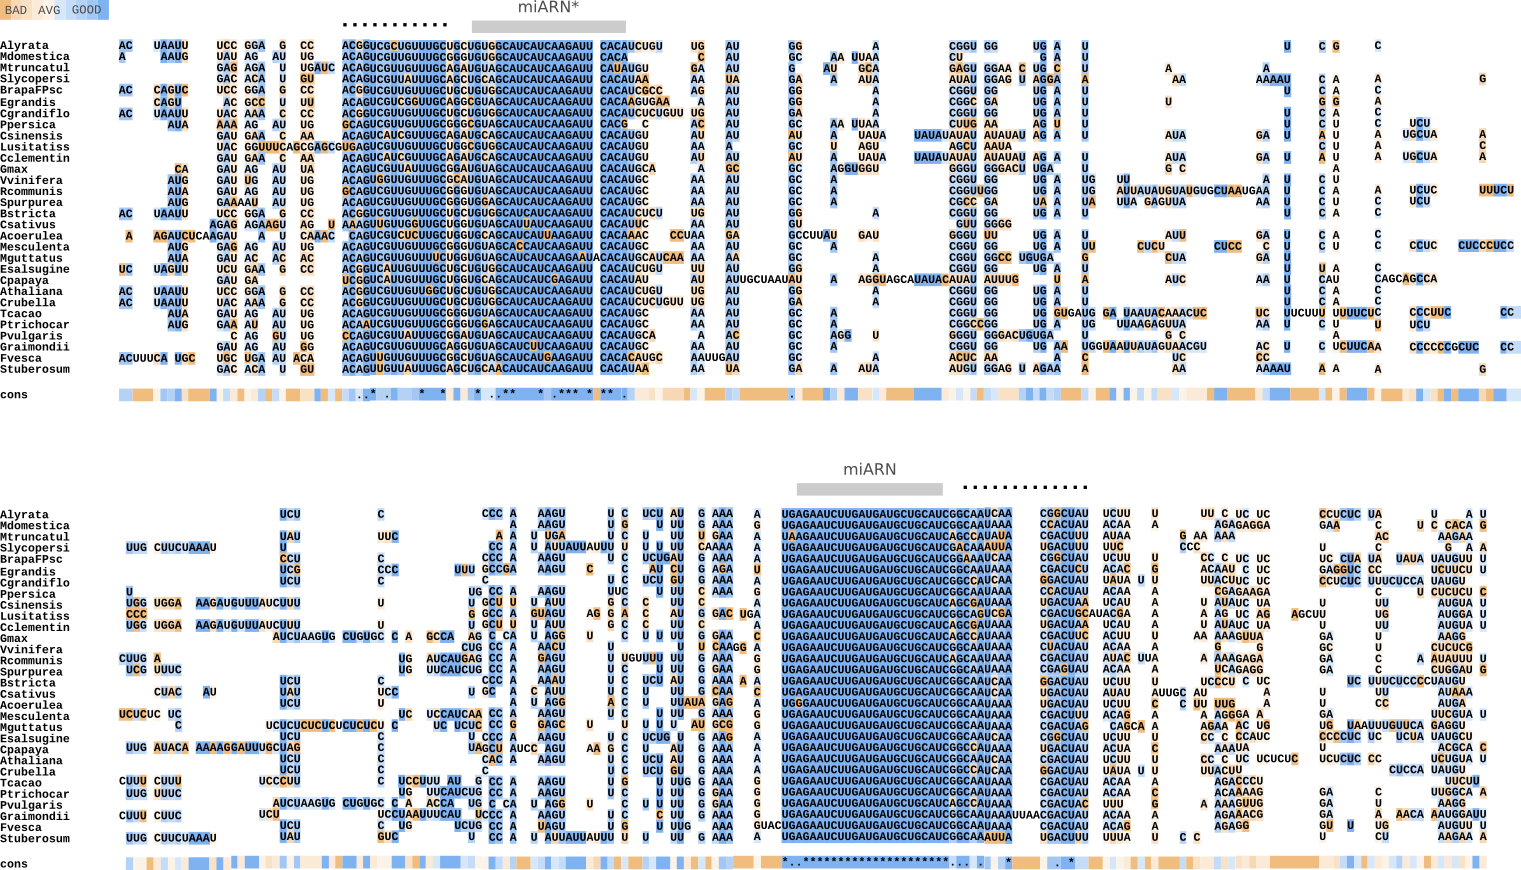
\includegraphics[width=1\textwidth]{img/miR172a_tcoffee_03.png}
	\end{center}
\end{frame}

\begin{frame}{Conservación del consenso en base al alineamiento de secuencia primaria}
	\begin{center}
		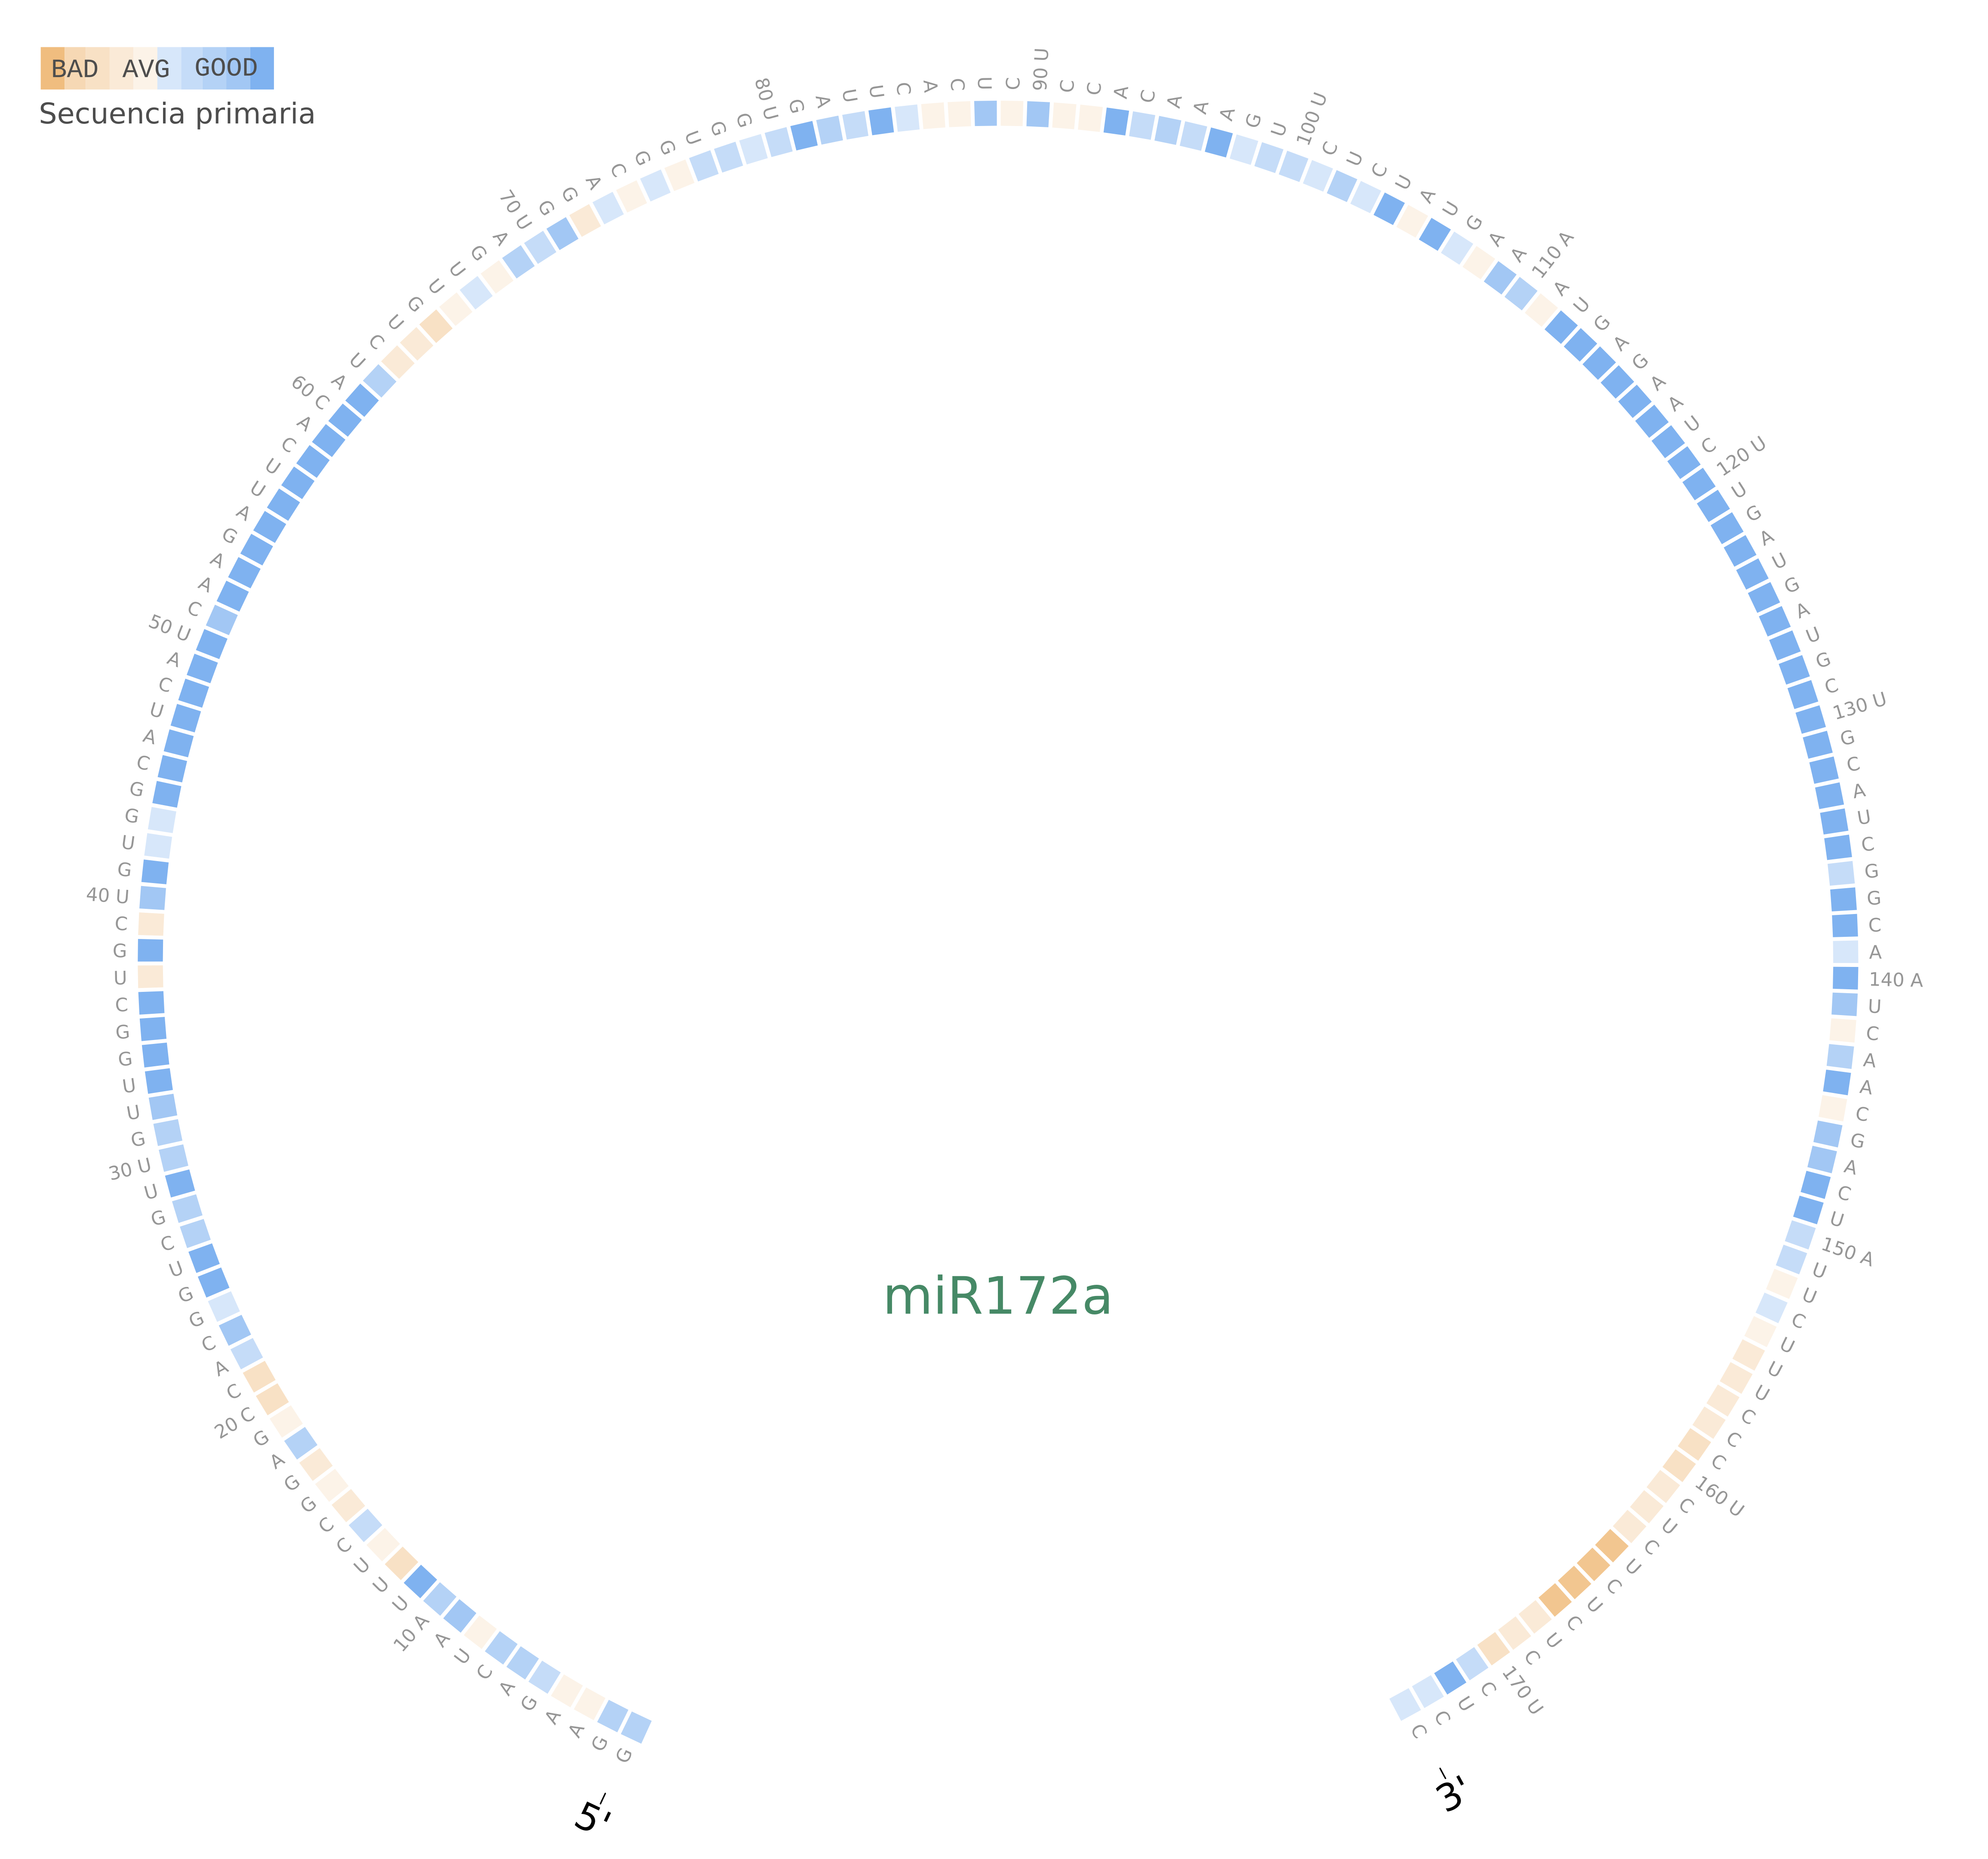
\includegraphics[width=.8\textwidth]{img/miR172a_circos01.png}
	\end{center}
\end{frame}

\begin{frame}{Frecuencia de bases apareadas y desapareadas}
	\begin{center}
		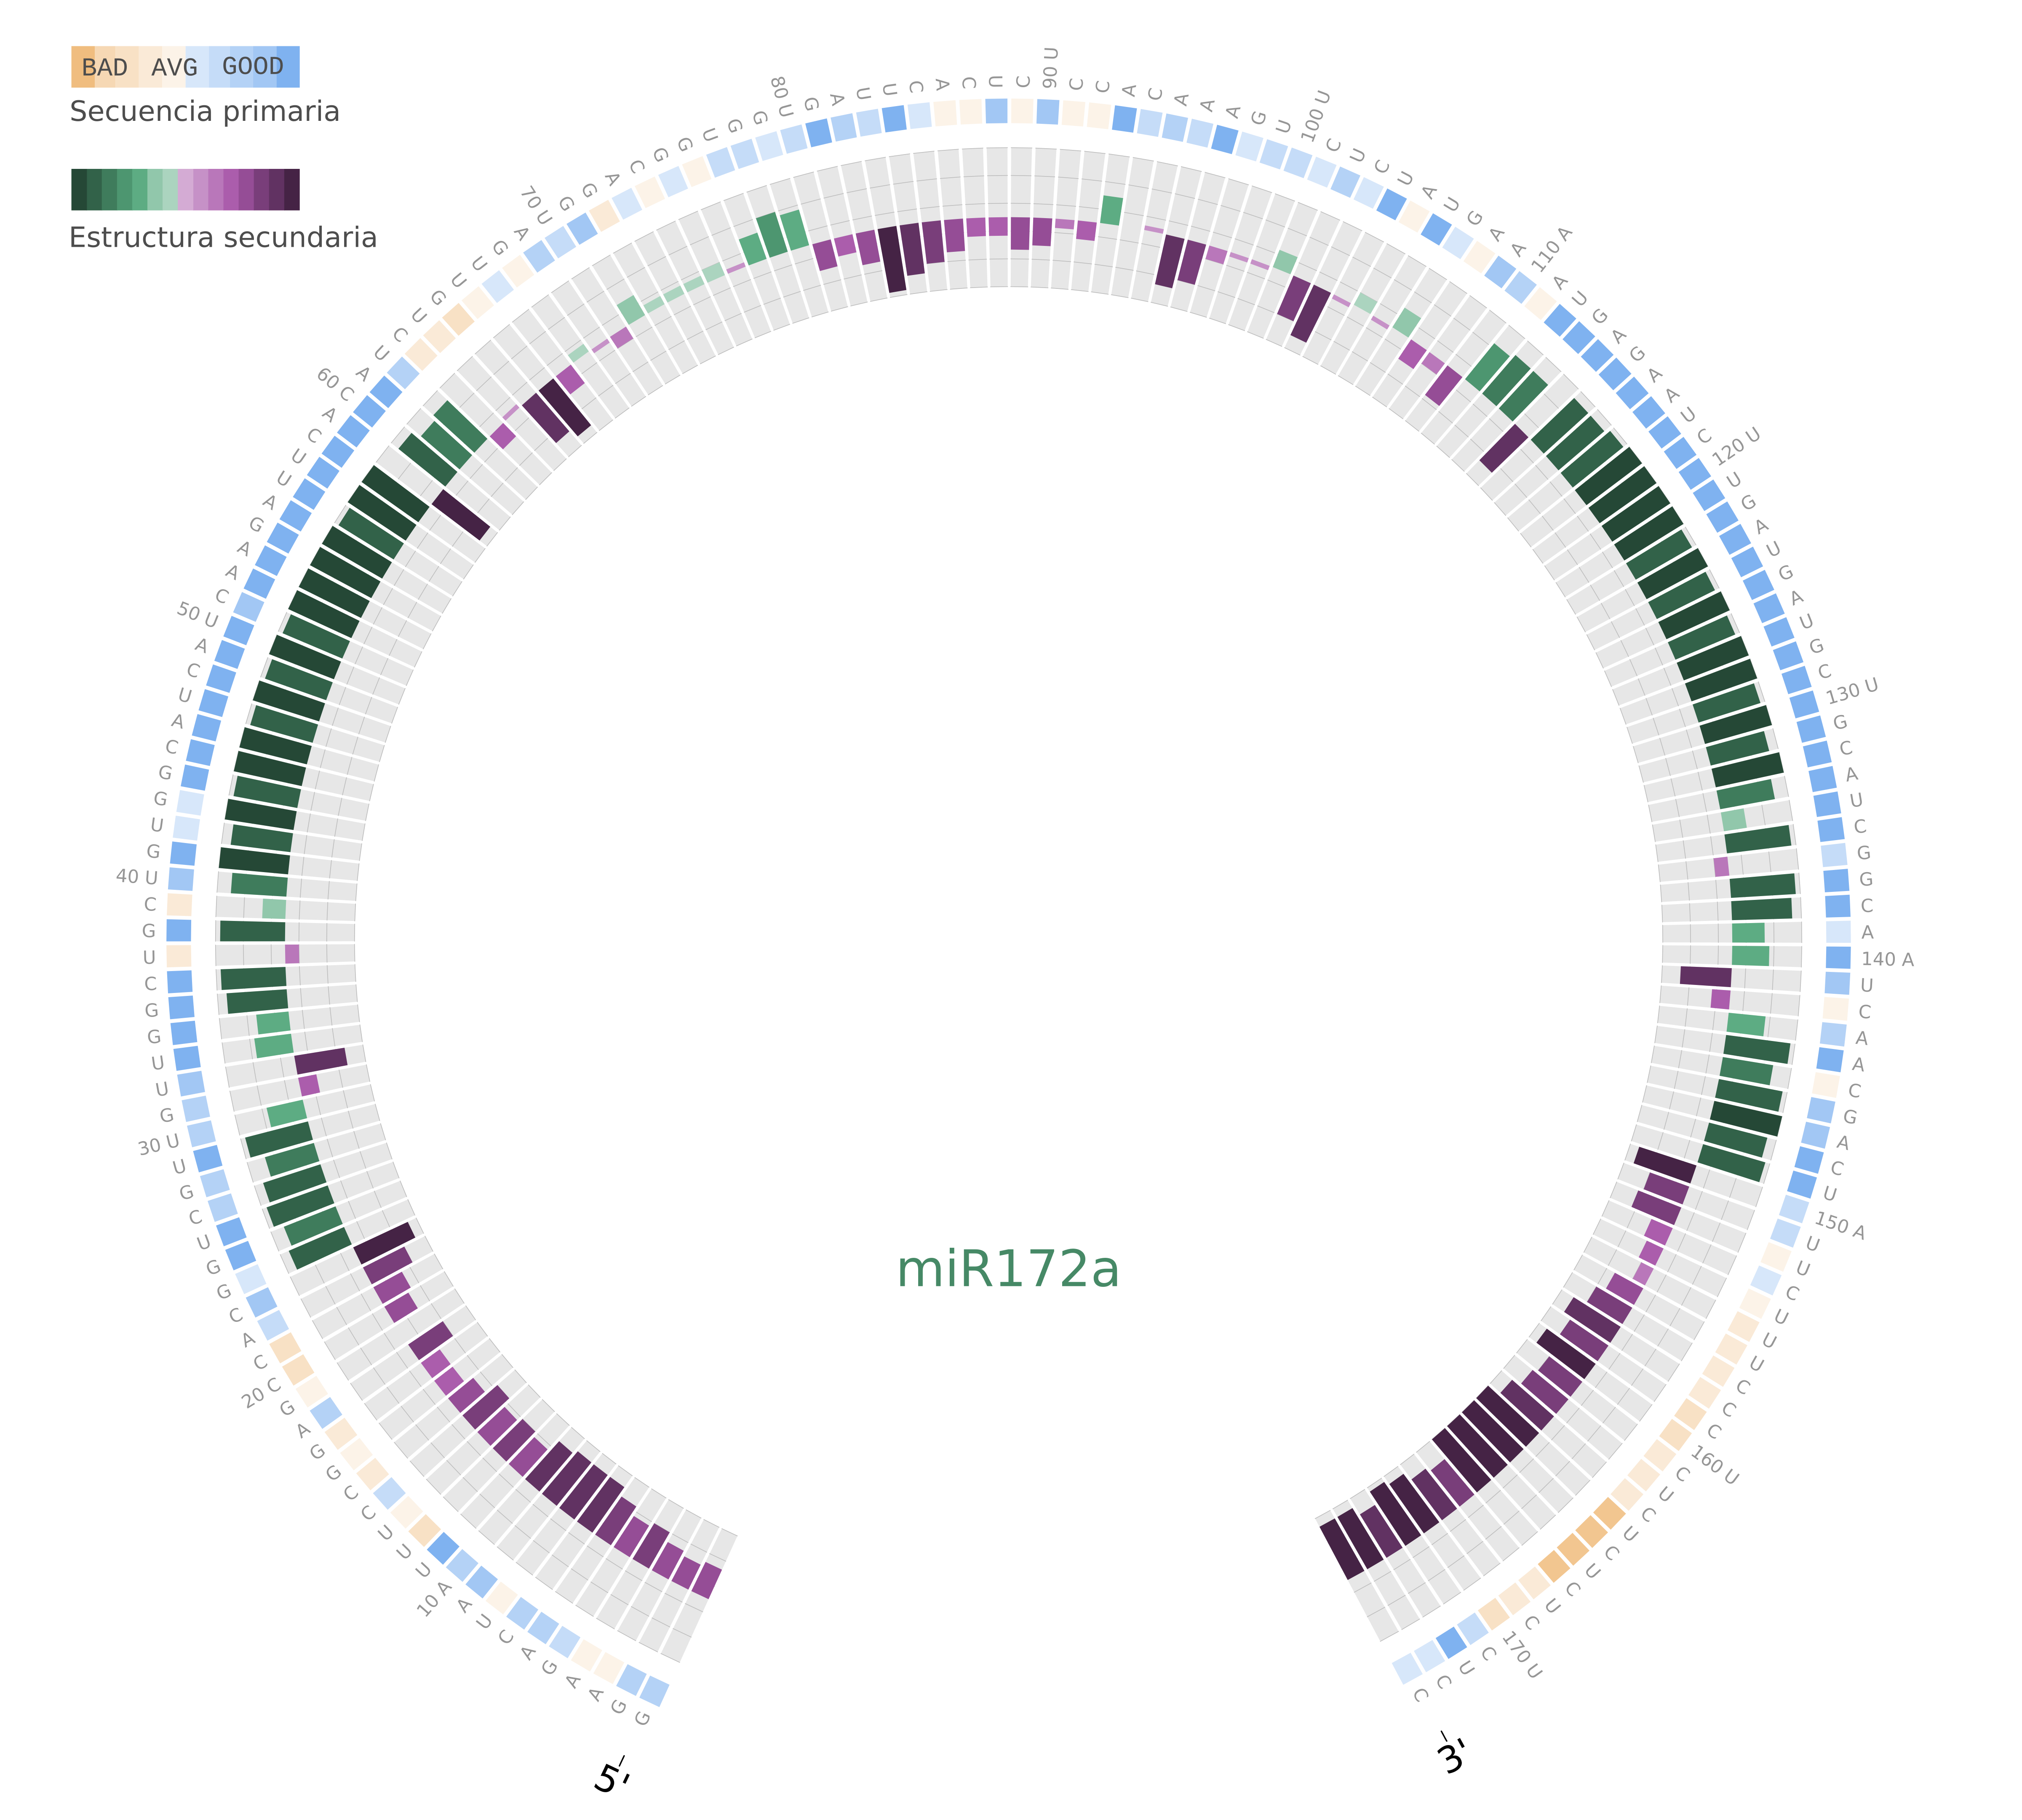
\includegraphics[width=.8\textwidth]{img/miR172a_circos02.png}
	\end{center}
\end{frame}

\begin{frame}{Interacción entre pares de bases considerando estructura secundaria}
	\begin{center}
		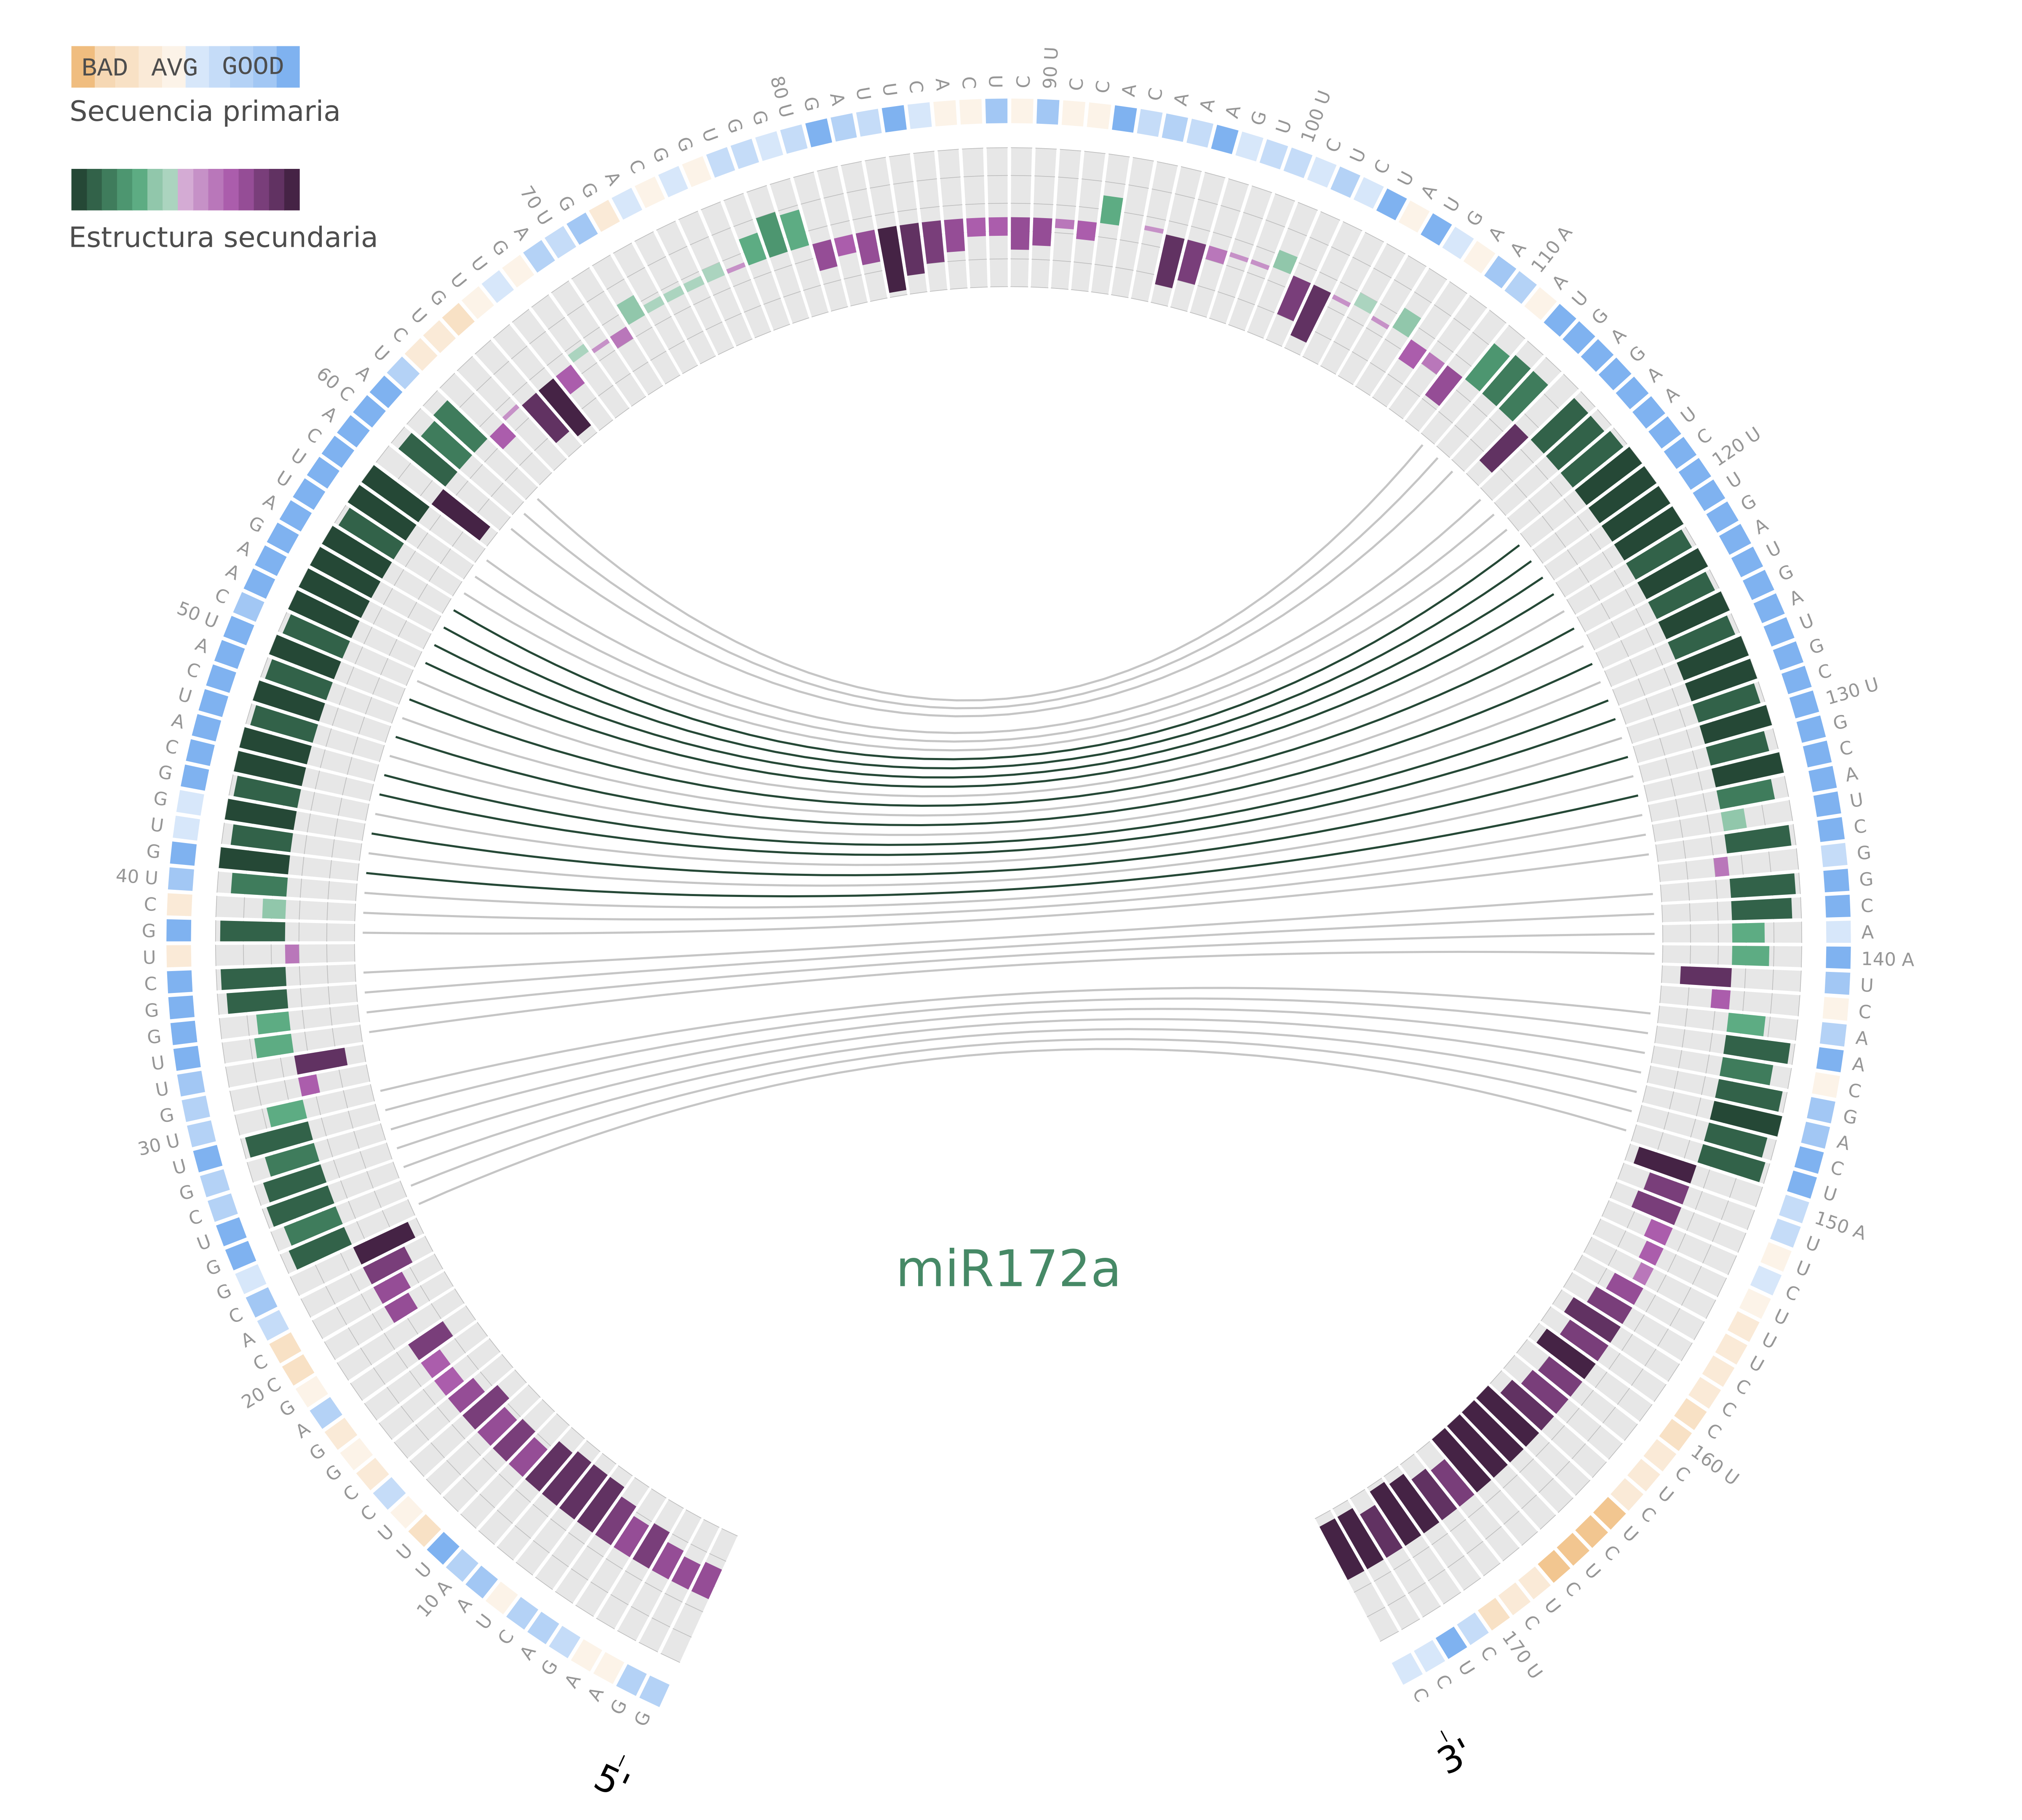
\includegraphics[width=.8\textwidth]{img/miR172a_circos03.png}
	\end{center}
\end{frame}

\begin{frame}{miARN y miARN* conservados en secuencia primaria y estructura}
	\begin{center}
		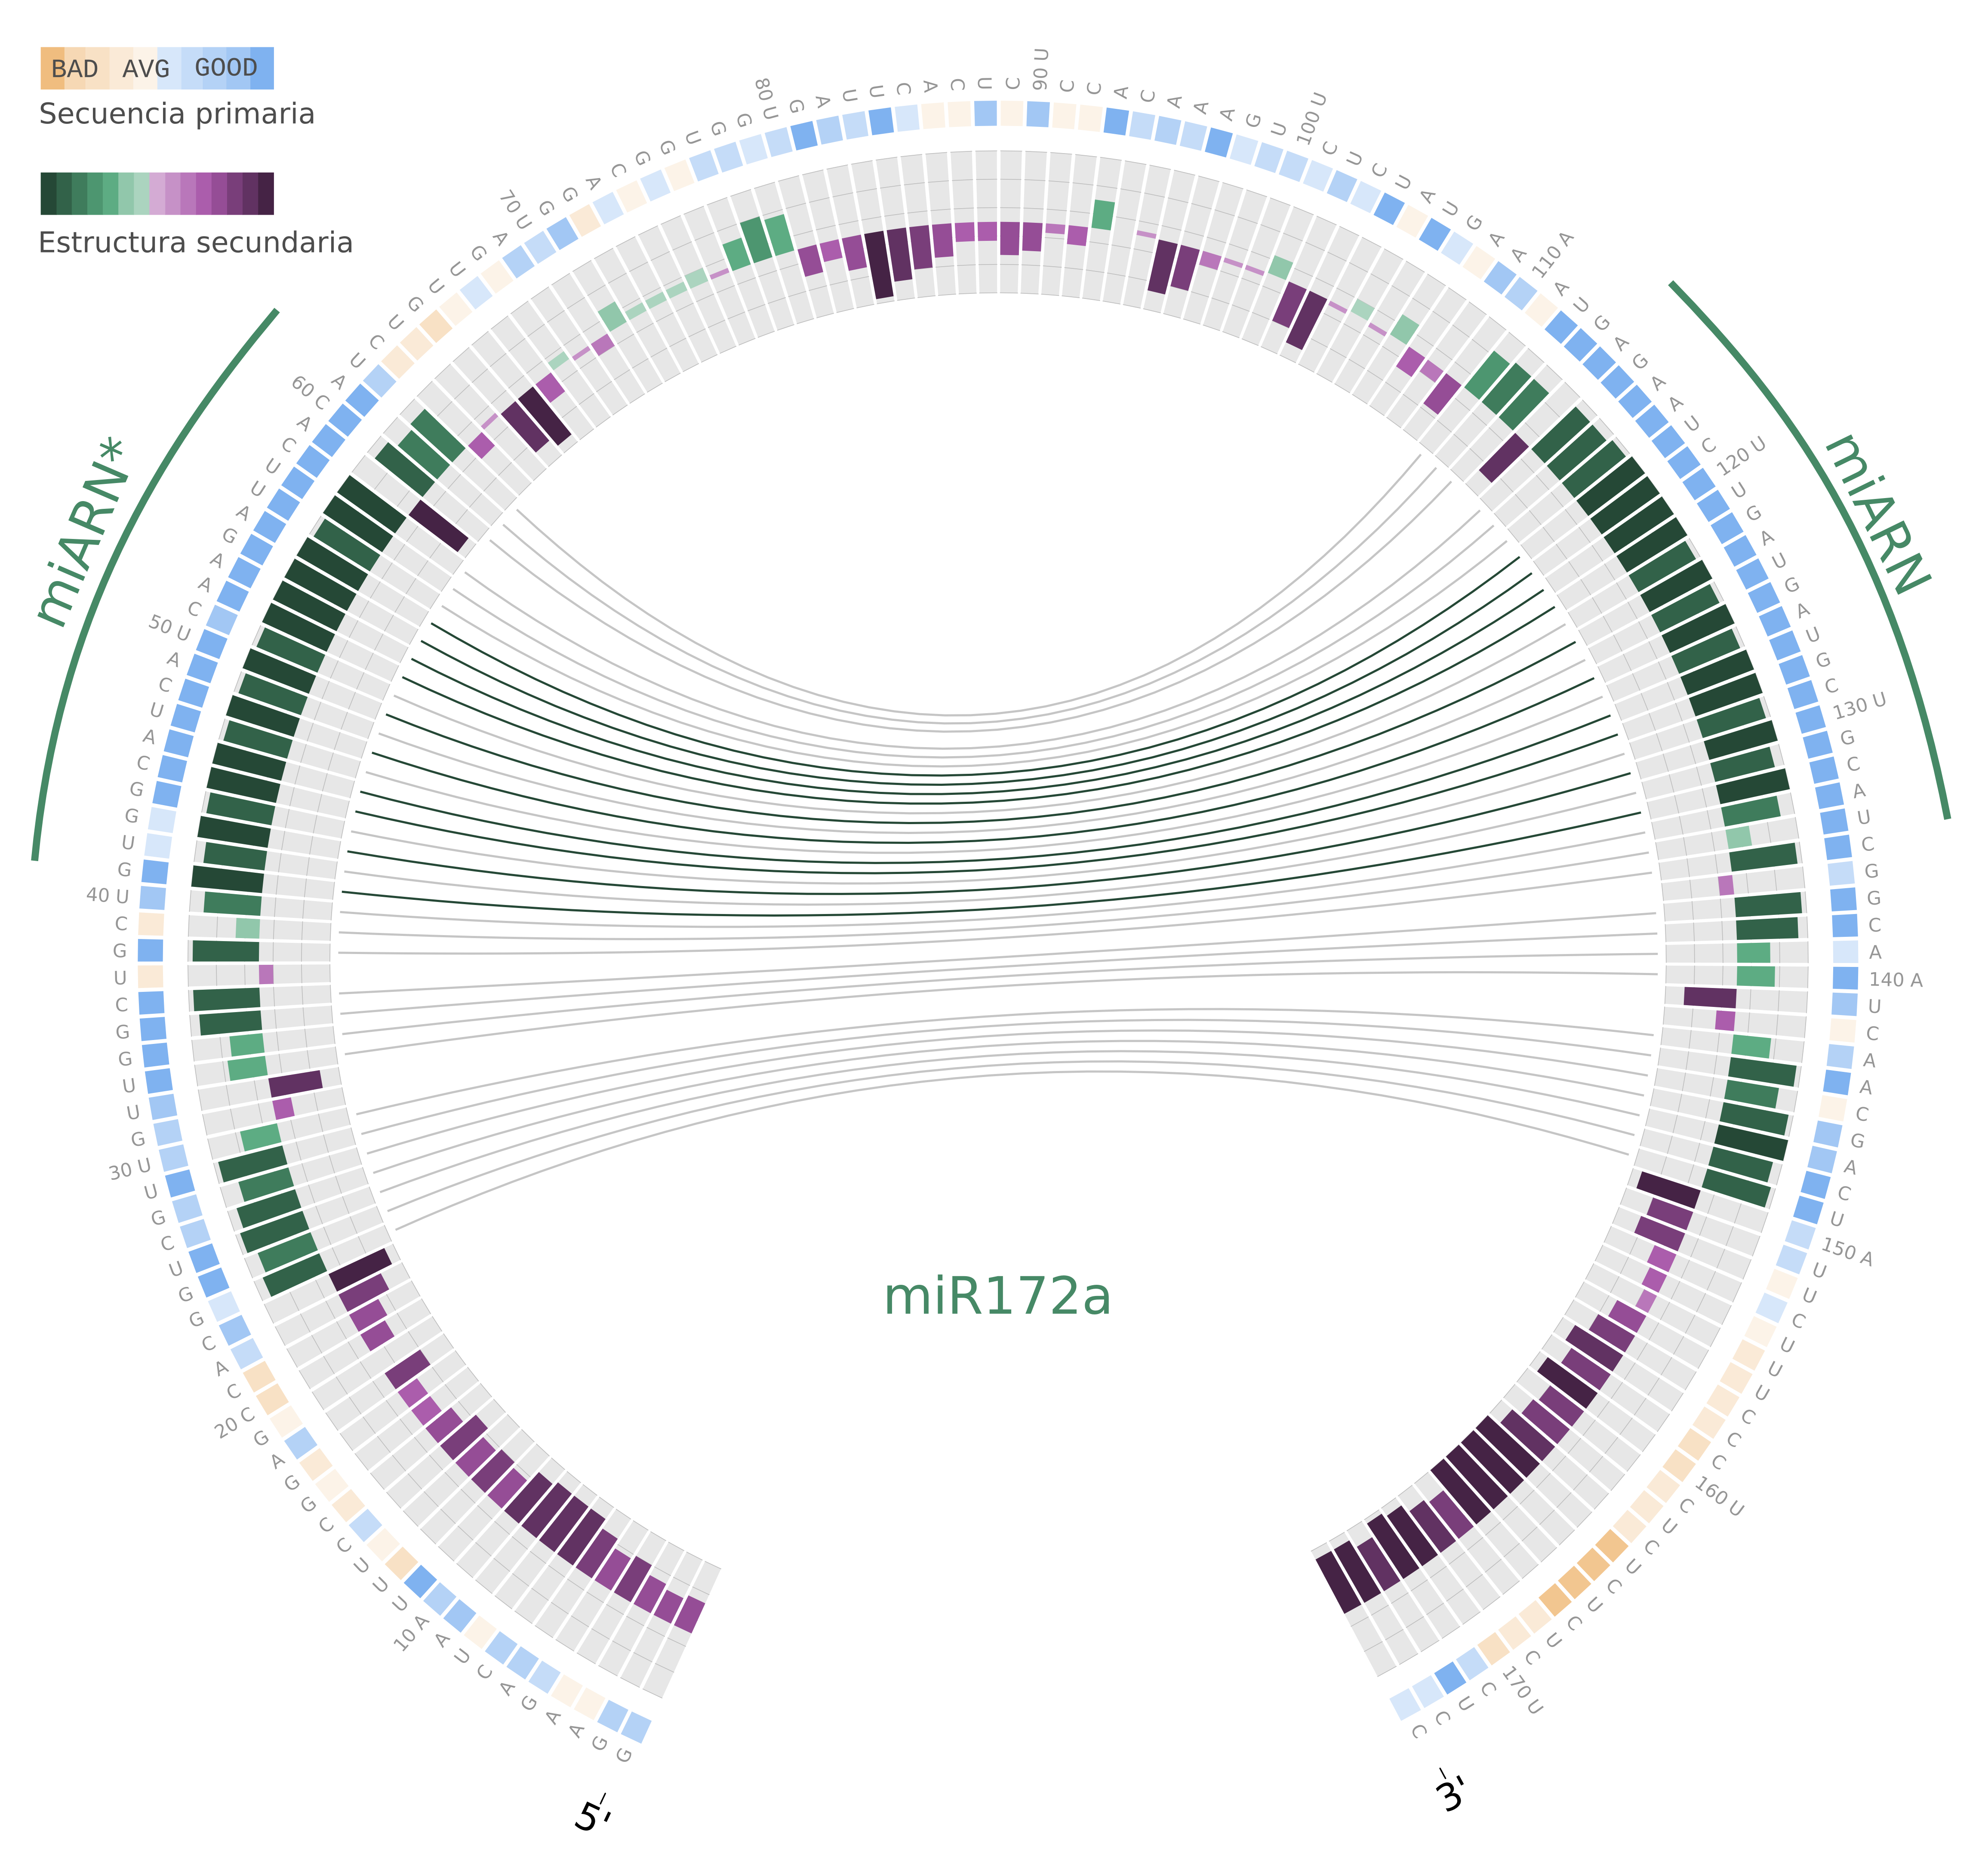
\includegraphics[width=.8\textwidth]{img/miR172a_circos04.png}
	\end{center}
\end{frame}

\begin{frame}{Región conservada por debajo del dúplex que coincide con el tallo inferior}
	\begin{center}
		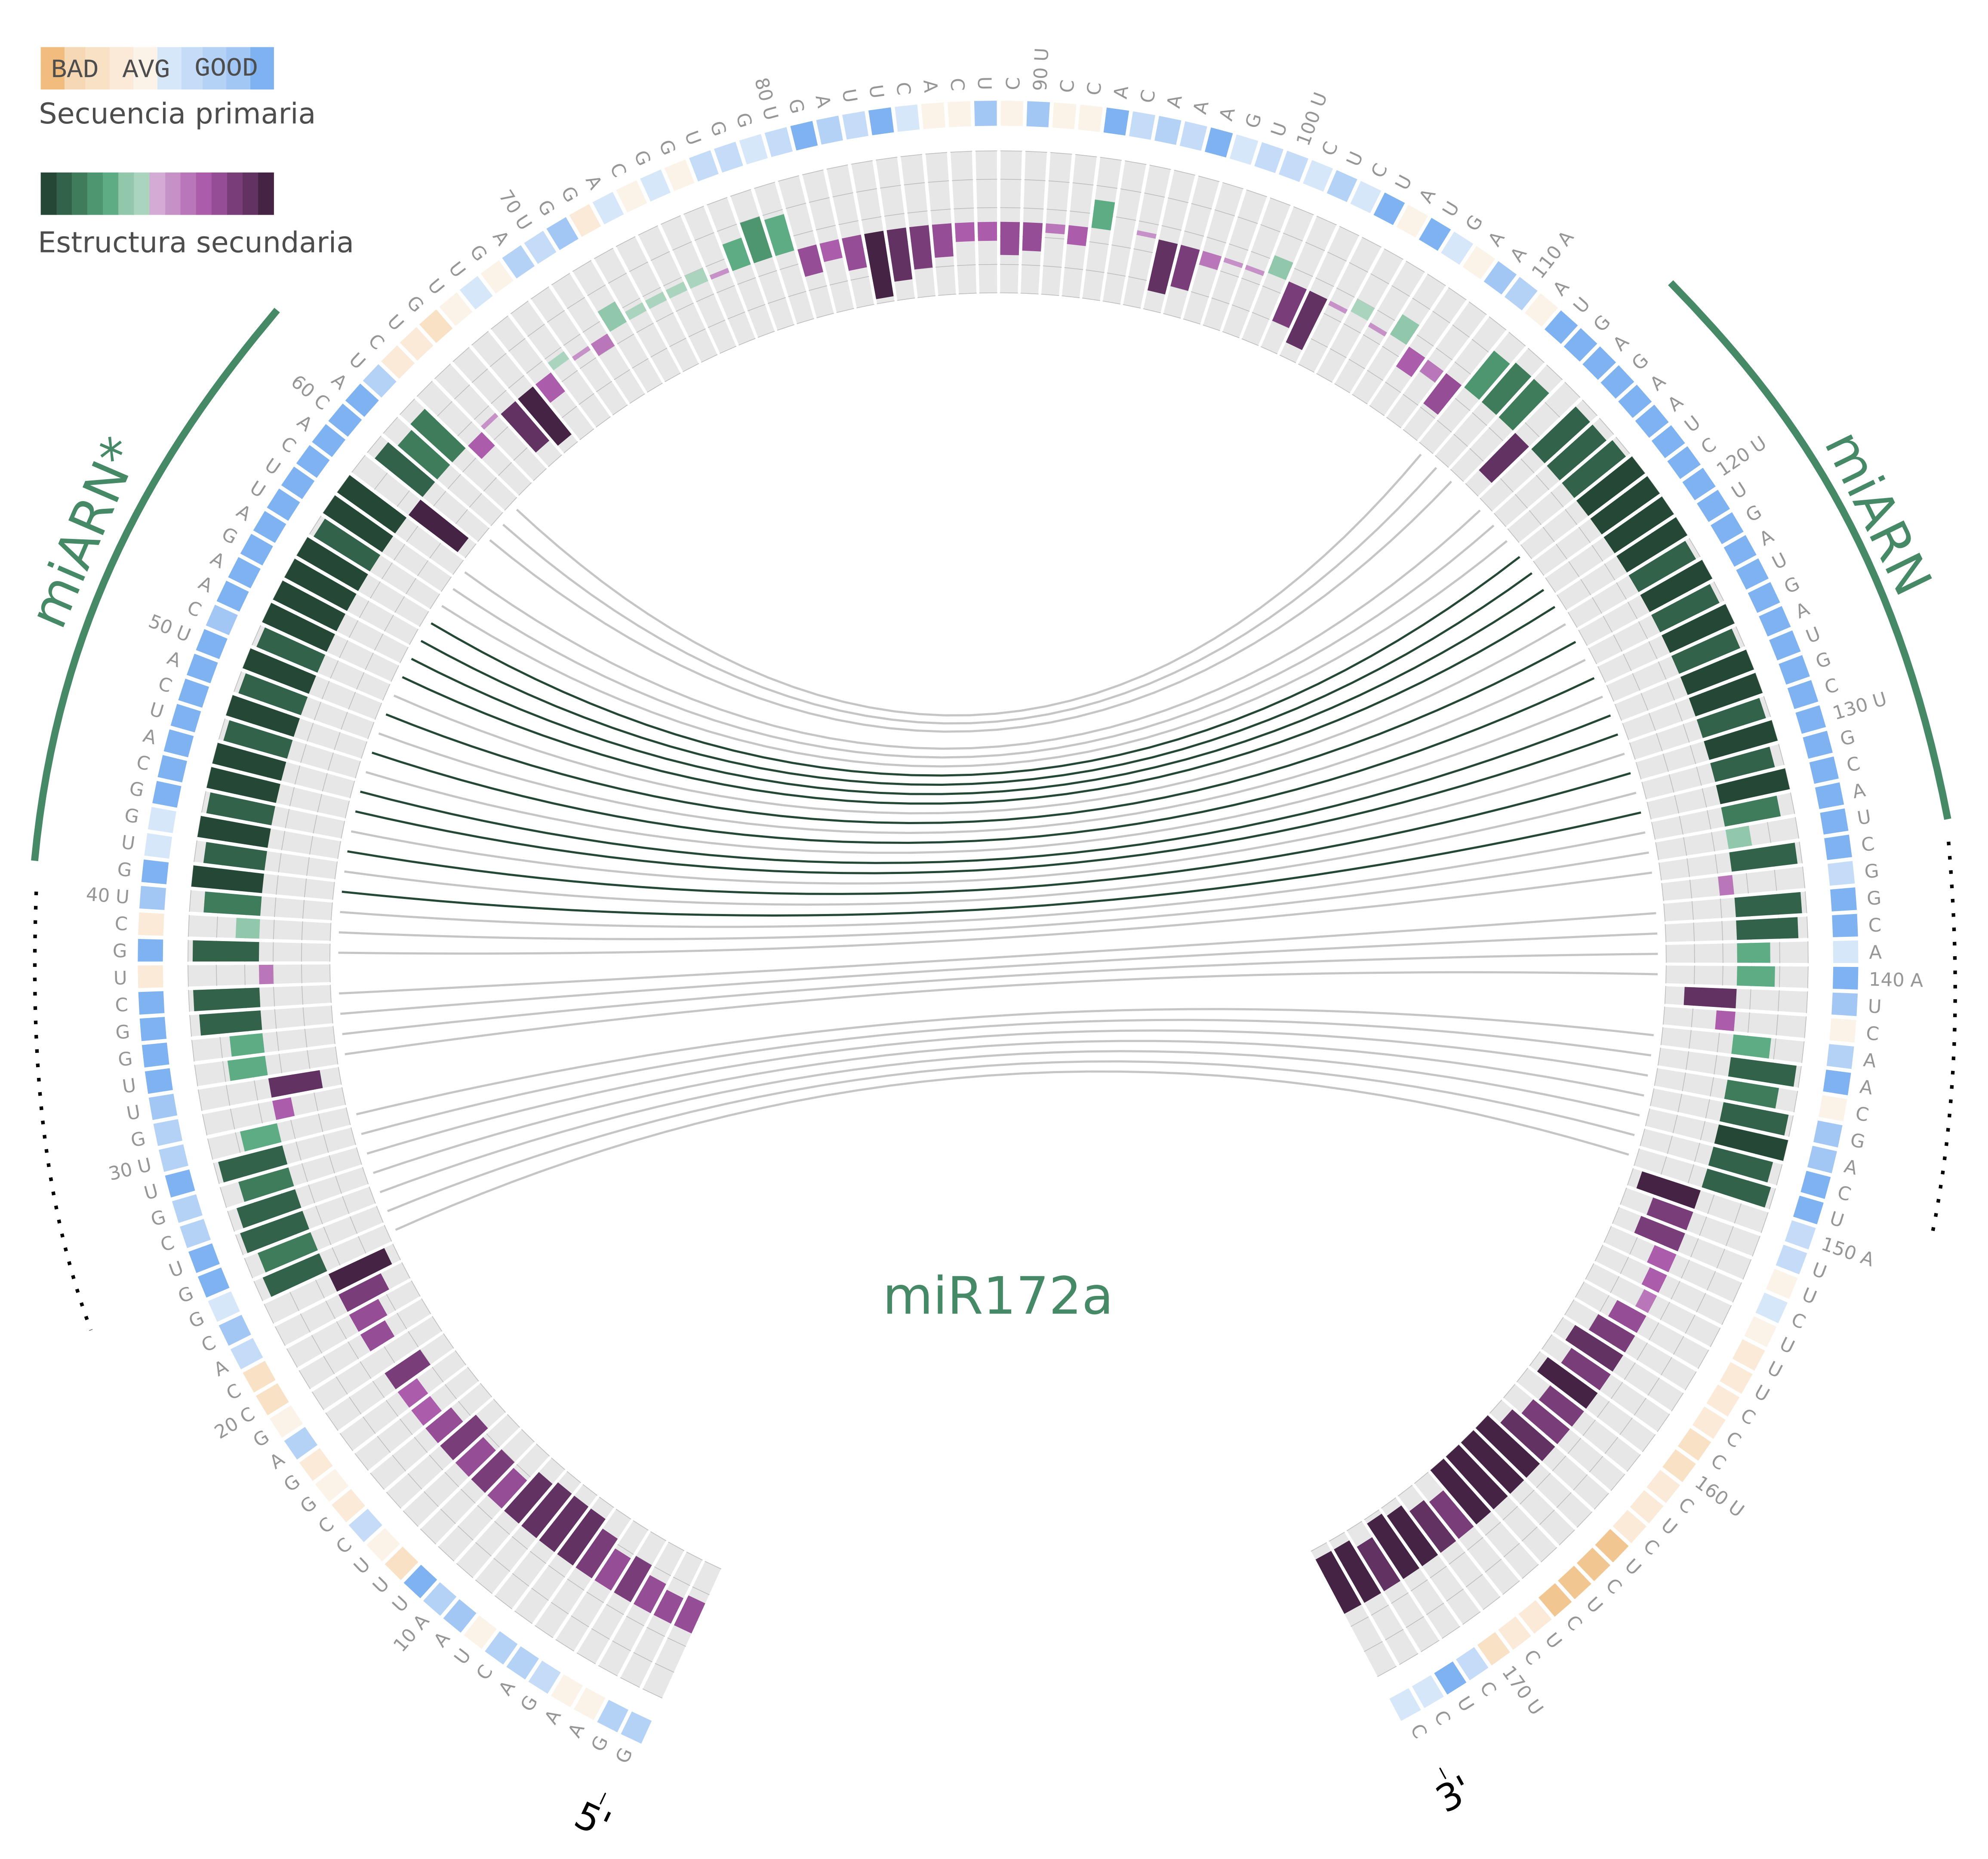
\includegraphics[width=.8\textwidth]{img/miR172a_circos05.png}
	\end{center}
\end{frame}

\begin{frame}{Mismatches conservados}
	\begin{center}
		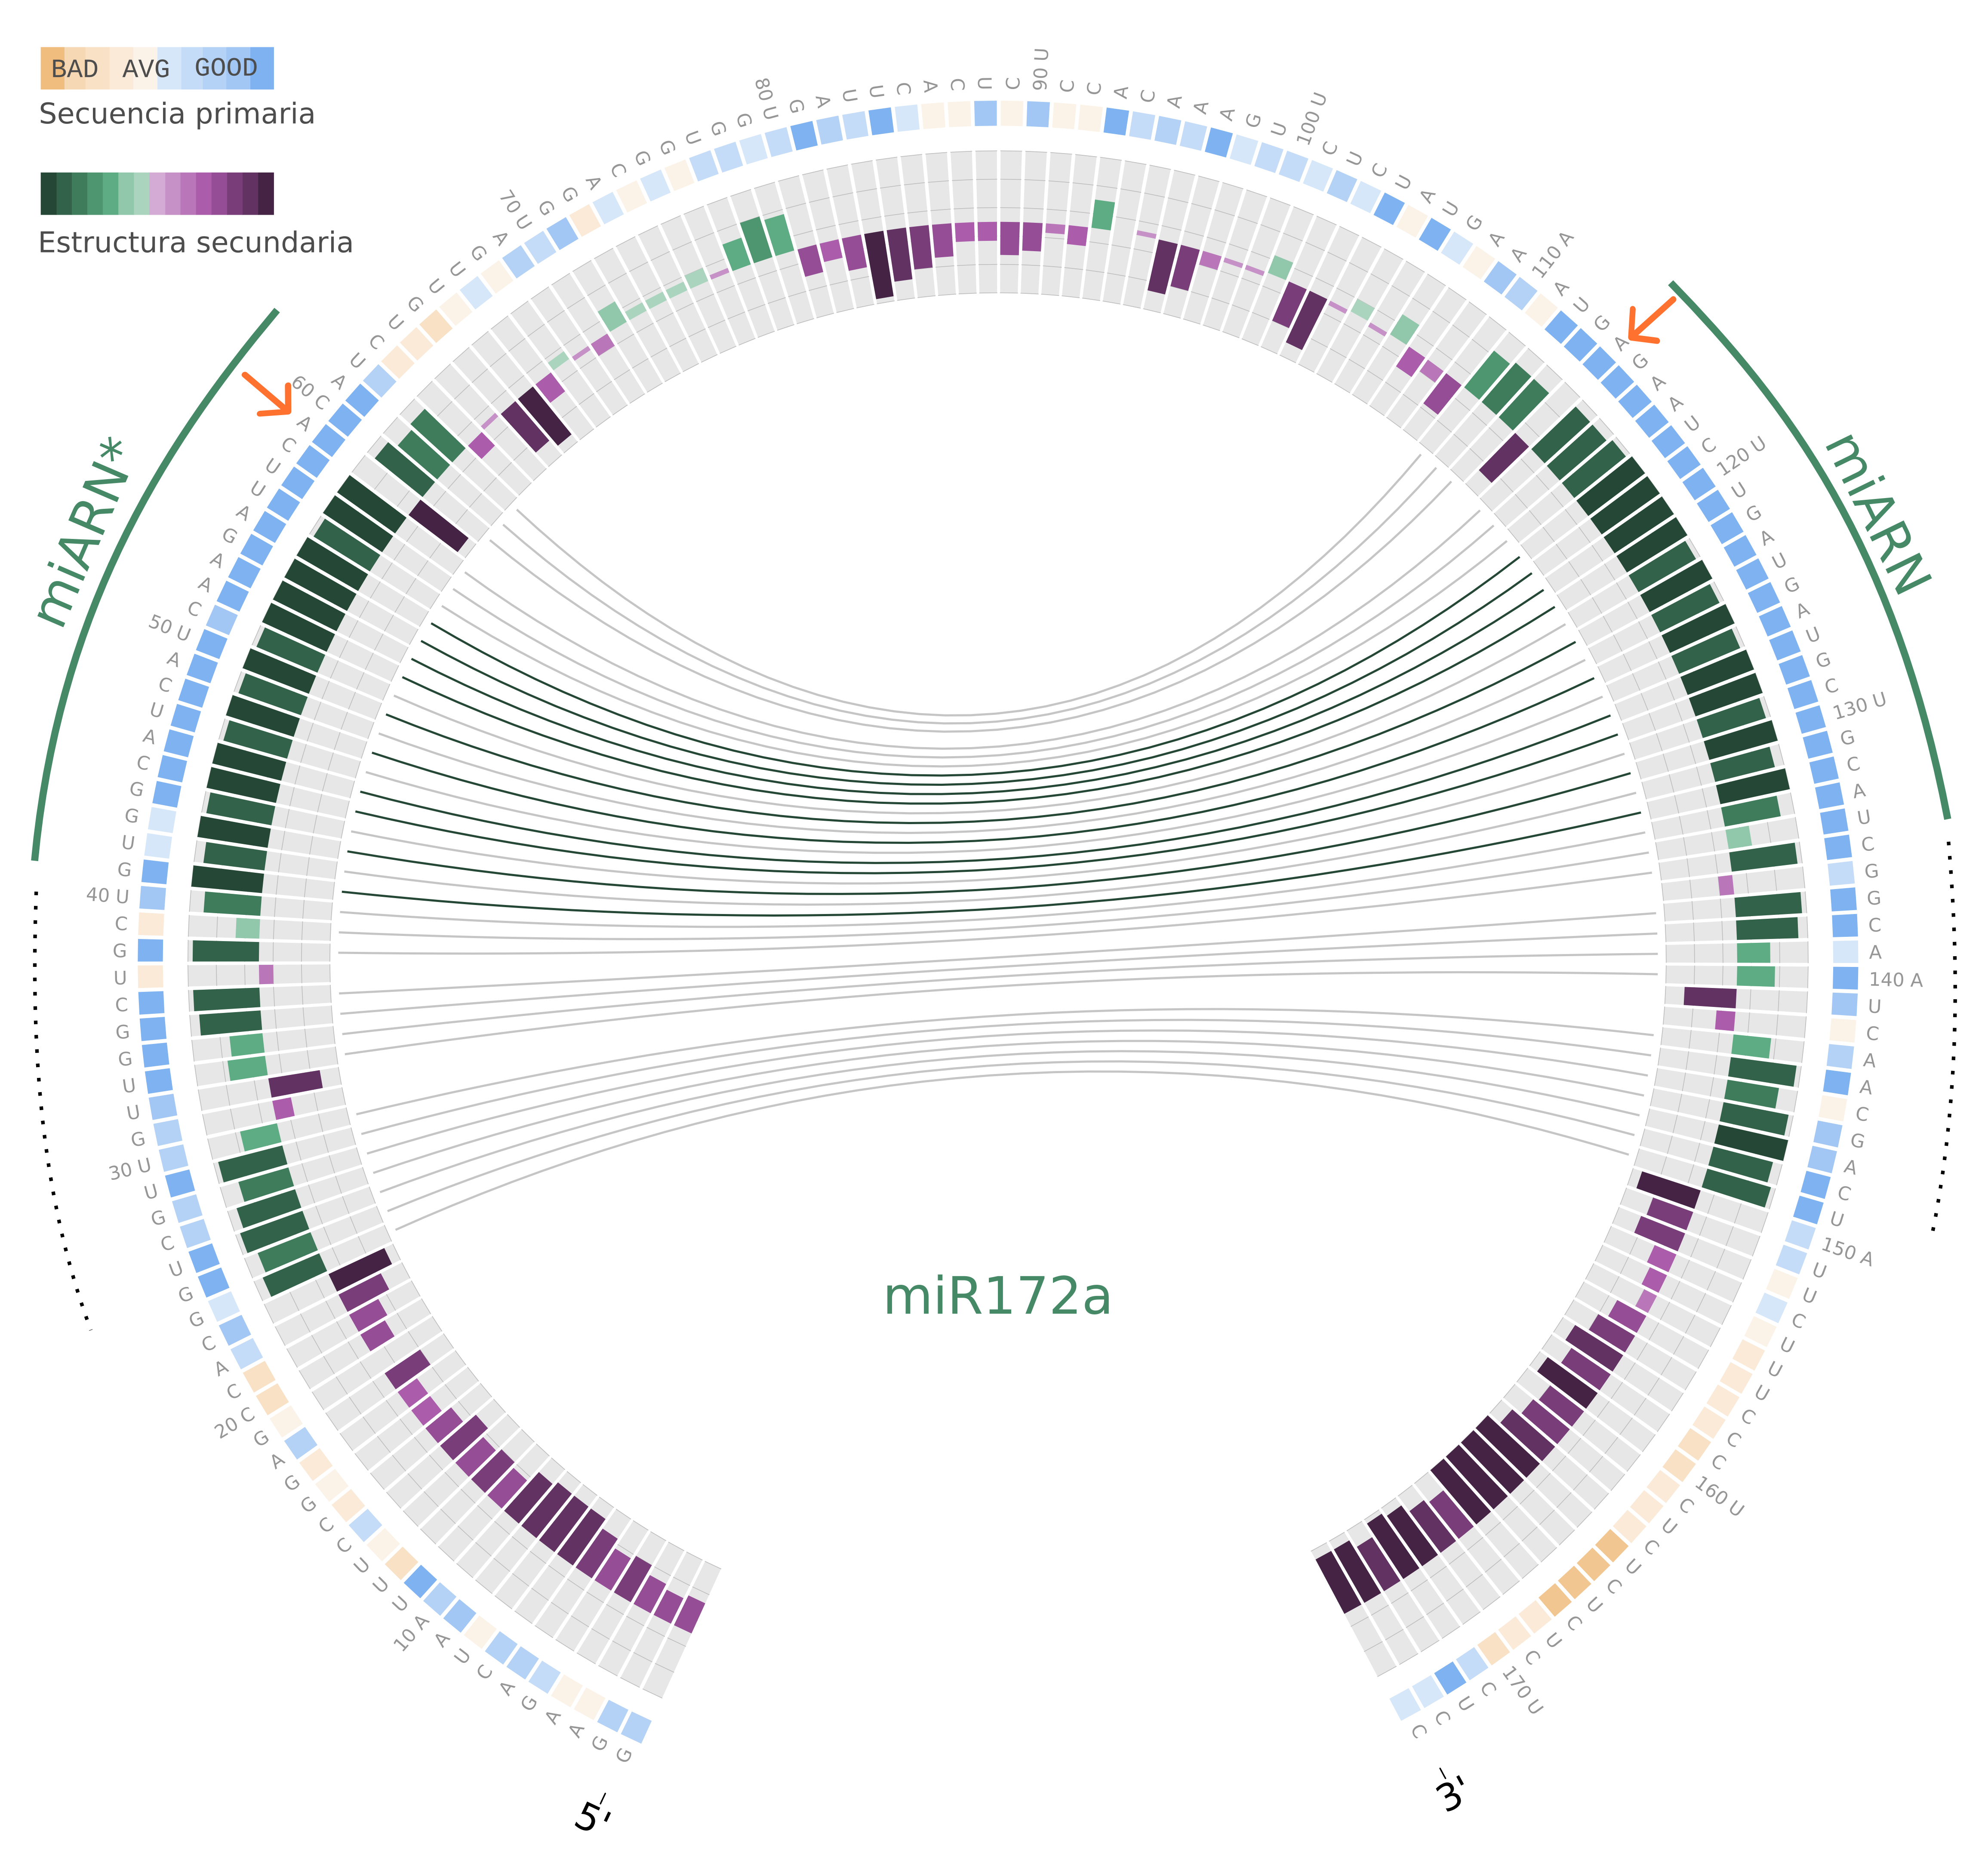
\includegraphics[width=.8\textwidth]{img/miR172a_circos06.png}
	\end{center}
\end{frame}

\begin{frame}{Mismo patrón de conservación en otros precursores que se procesan desde la base}
	\begin{center}
		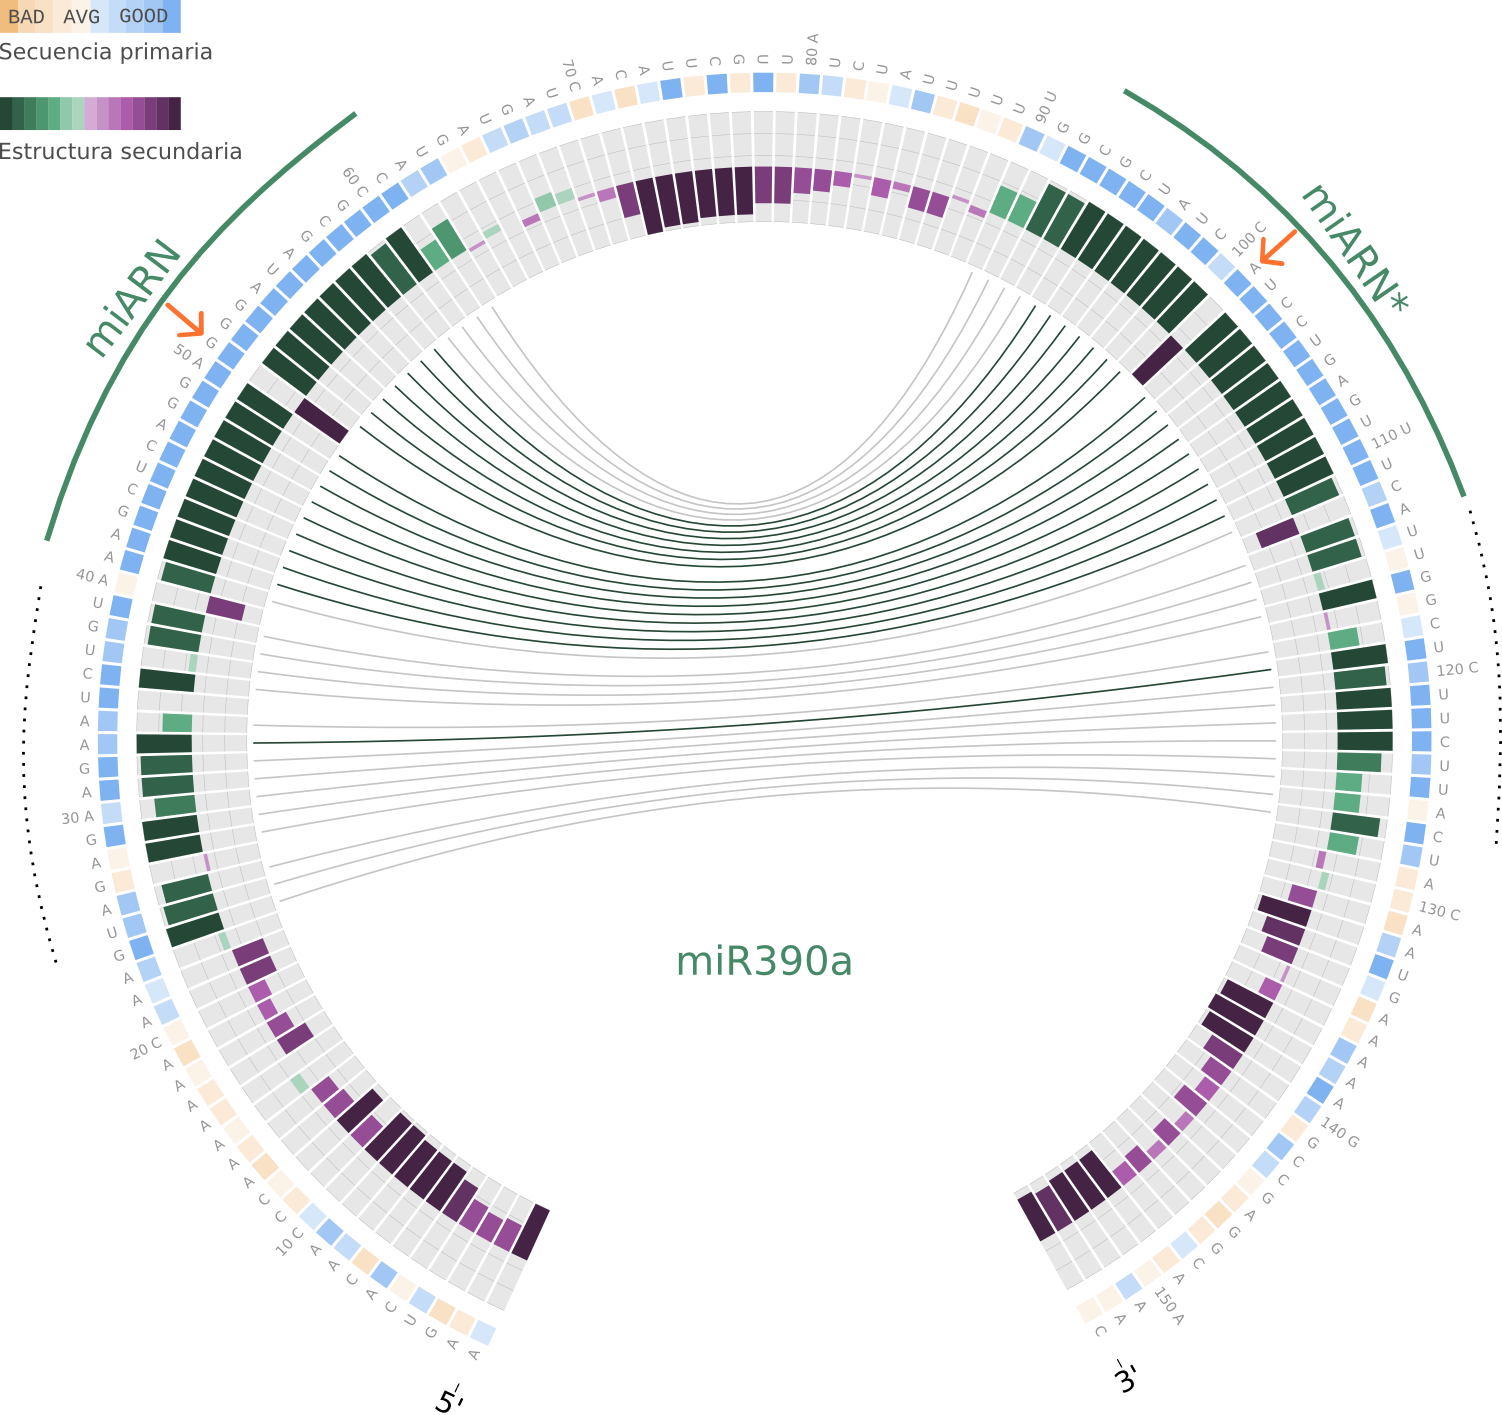
\includegraphics[width=.7\textwidth]{img/miR390a_circos.png}
	\end{center}
\end{frame}

\begin{frame}{Precursores que se procesan desde la base en forma secuencial}
	\begin{center}
		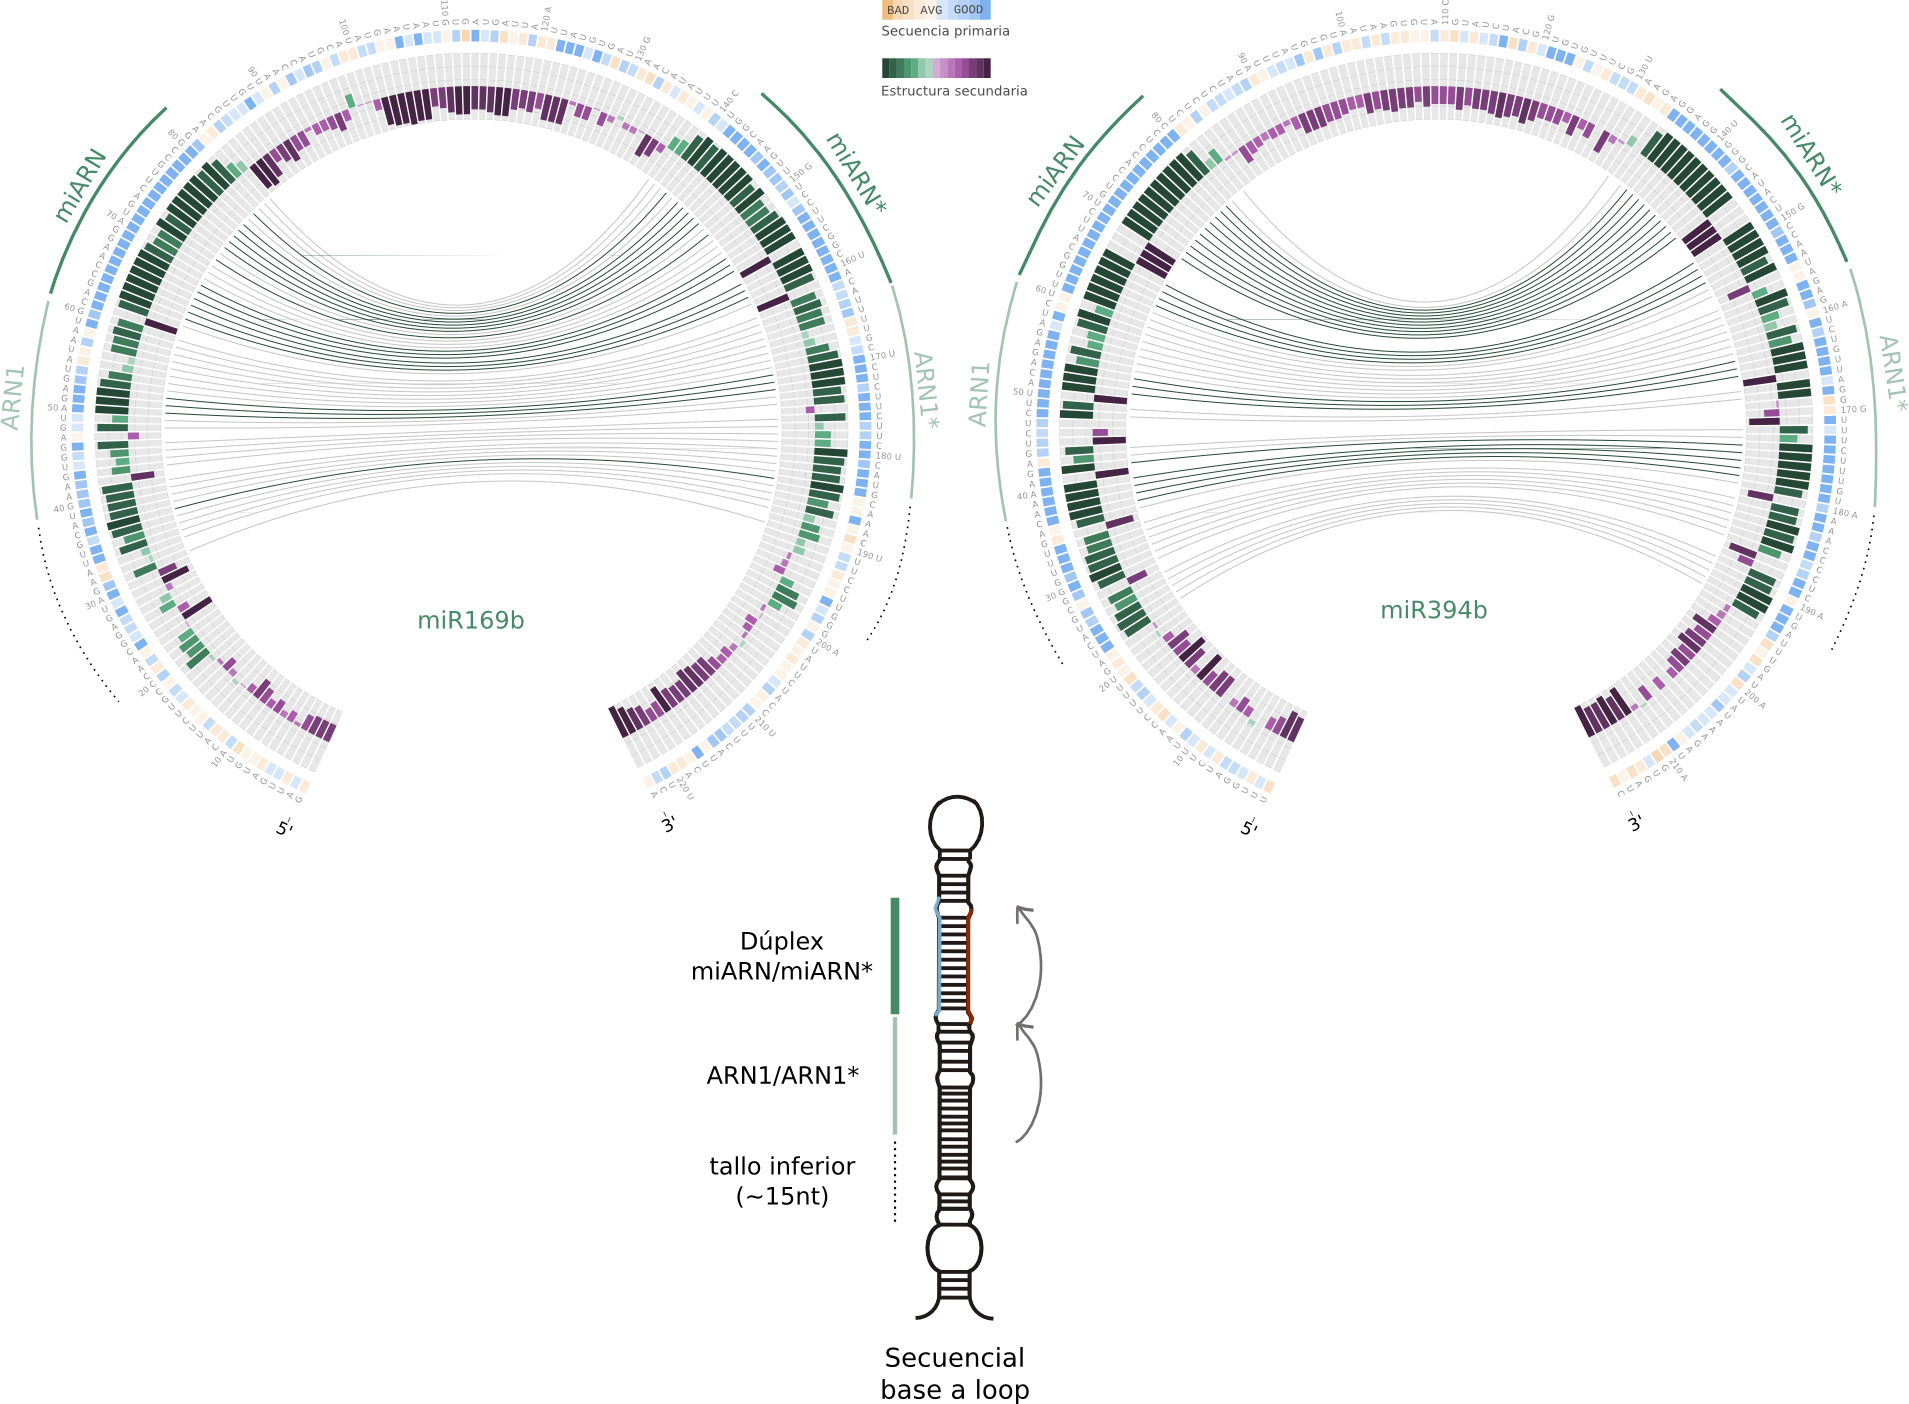
\includegraphics[width=1\textwidth]{img/seqBTL_circos.png}
	\end{center}
\end{frame}

\begin{frame}{cortos LTB}
	\begin{center}
		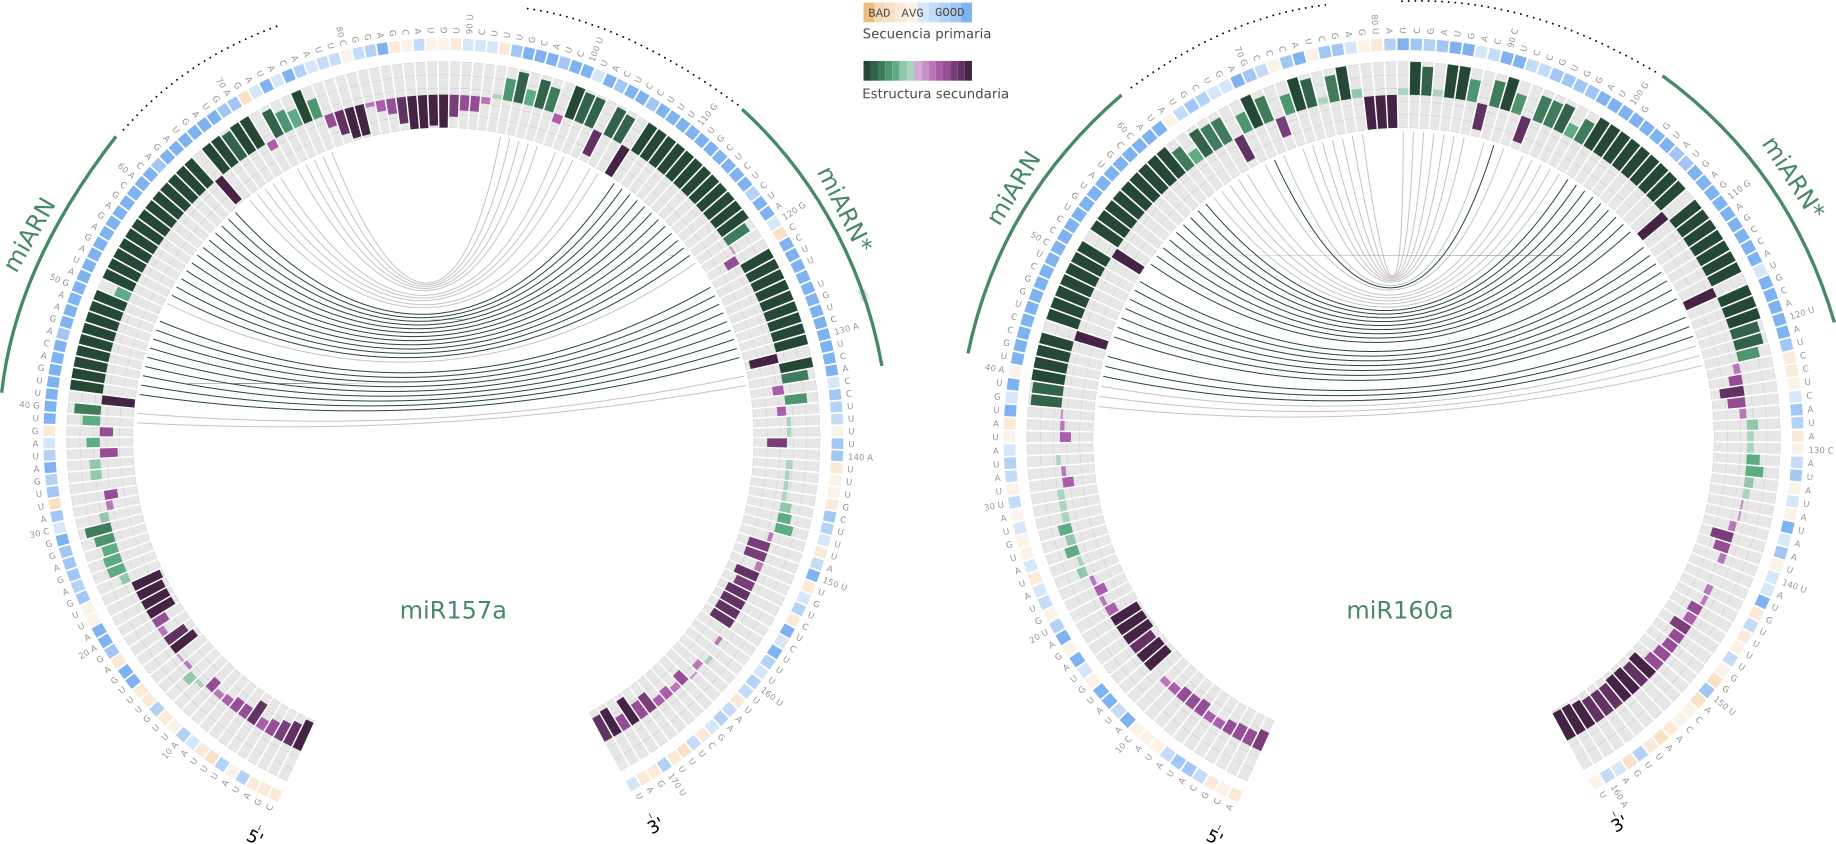
\includegraphics[width=1\textwidth]{img/srLTB_circos.png}
	\end{center}
\end{frame}

\begin{frame}{Seq LTB}
	\begin{center}
		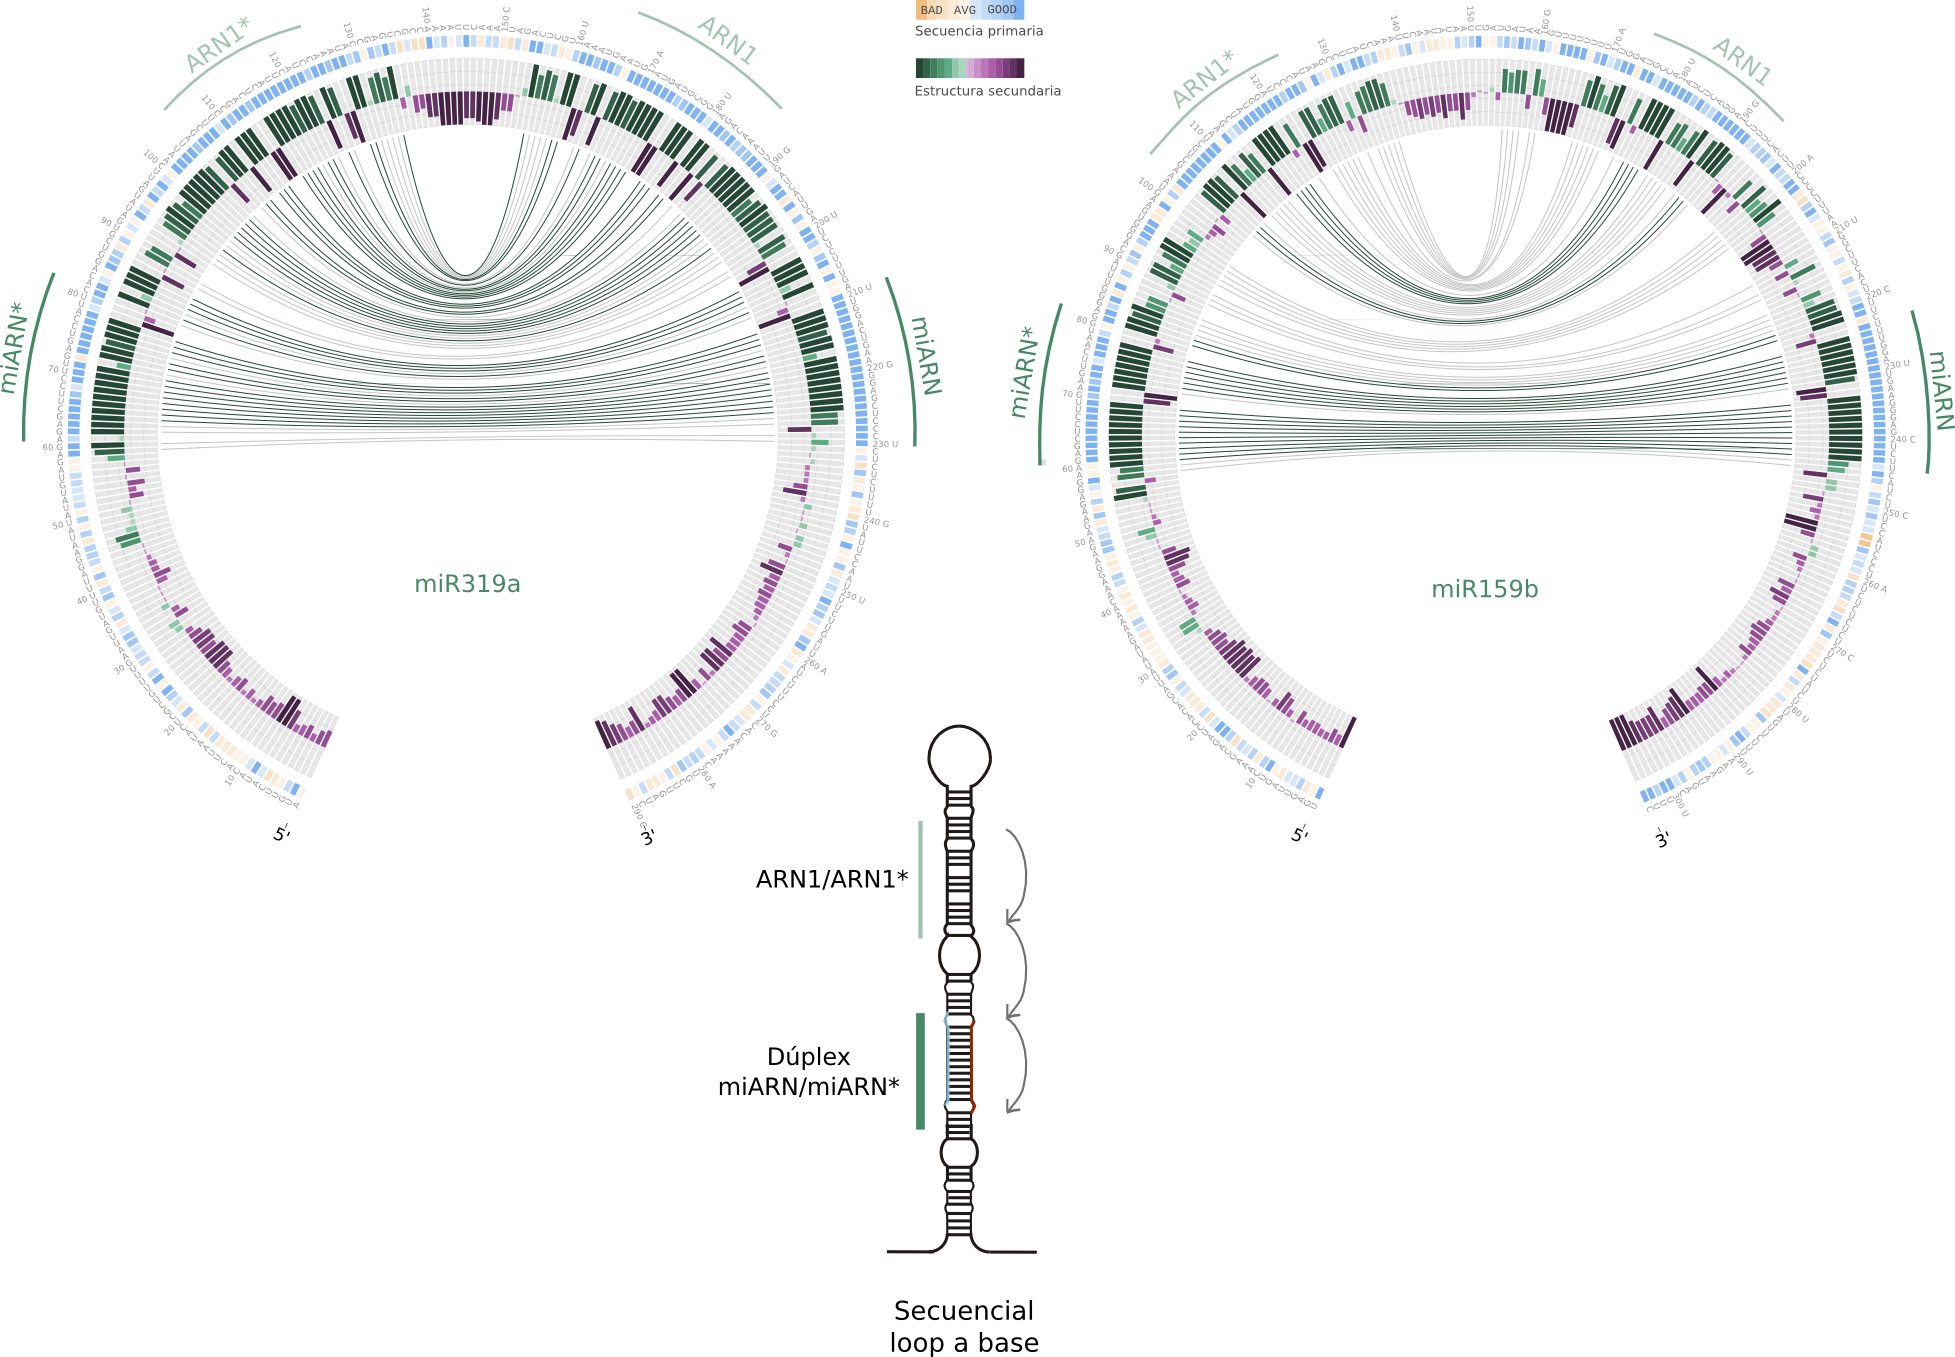
\includegraphics[width=1\textwidth]{img/seqLTB_circos.png}
	\end{center}
\end{frame}

\begin{frame}{En precursores que se procesan desde el loop, el tamaño del tallo superior el loop no varía en distintas especies}
	\begin{center}
		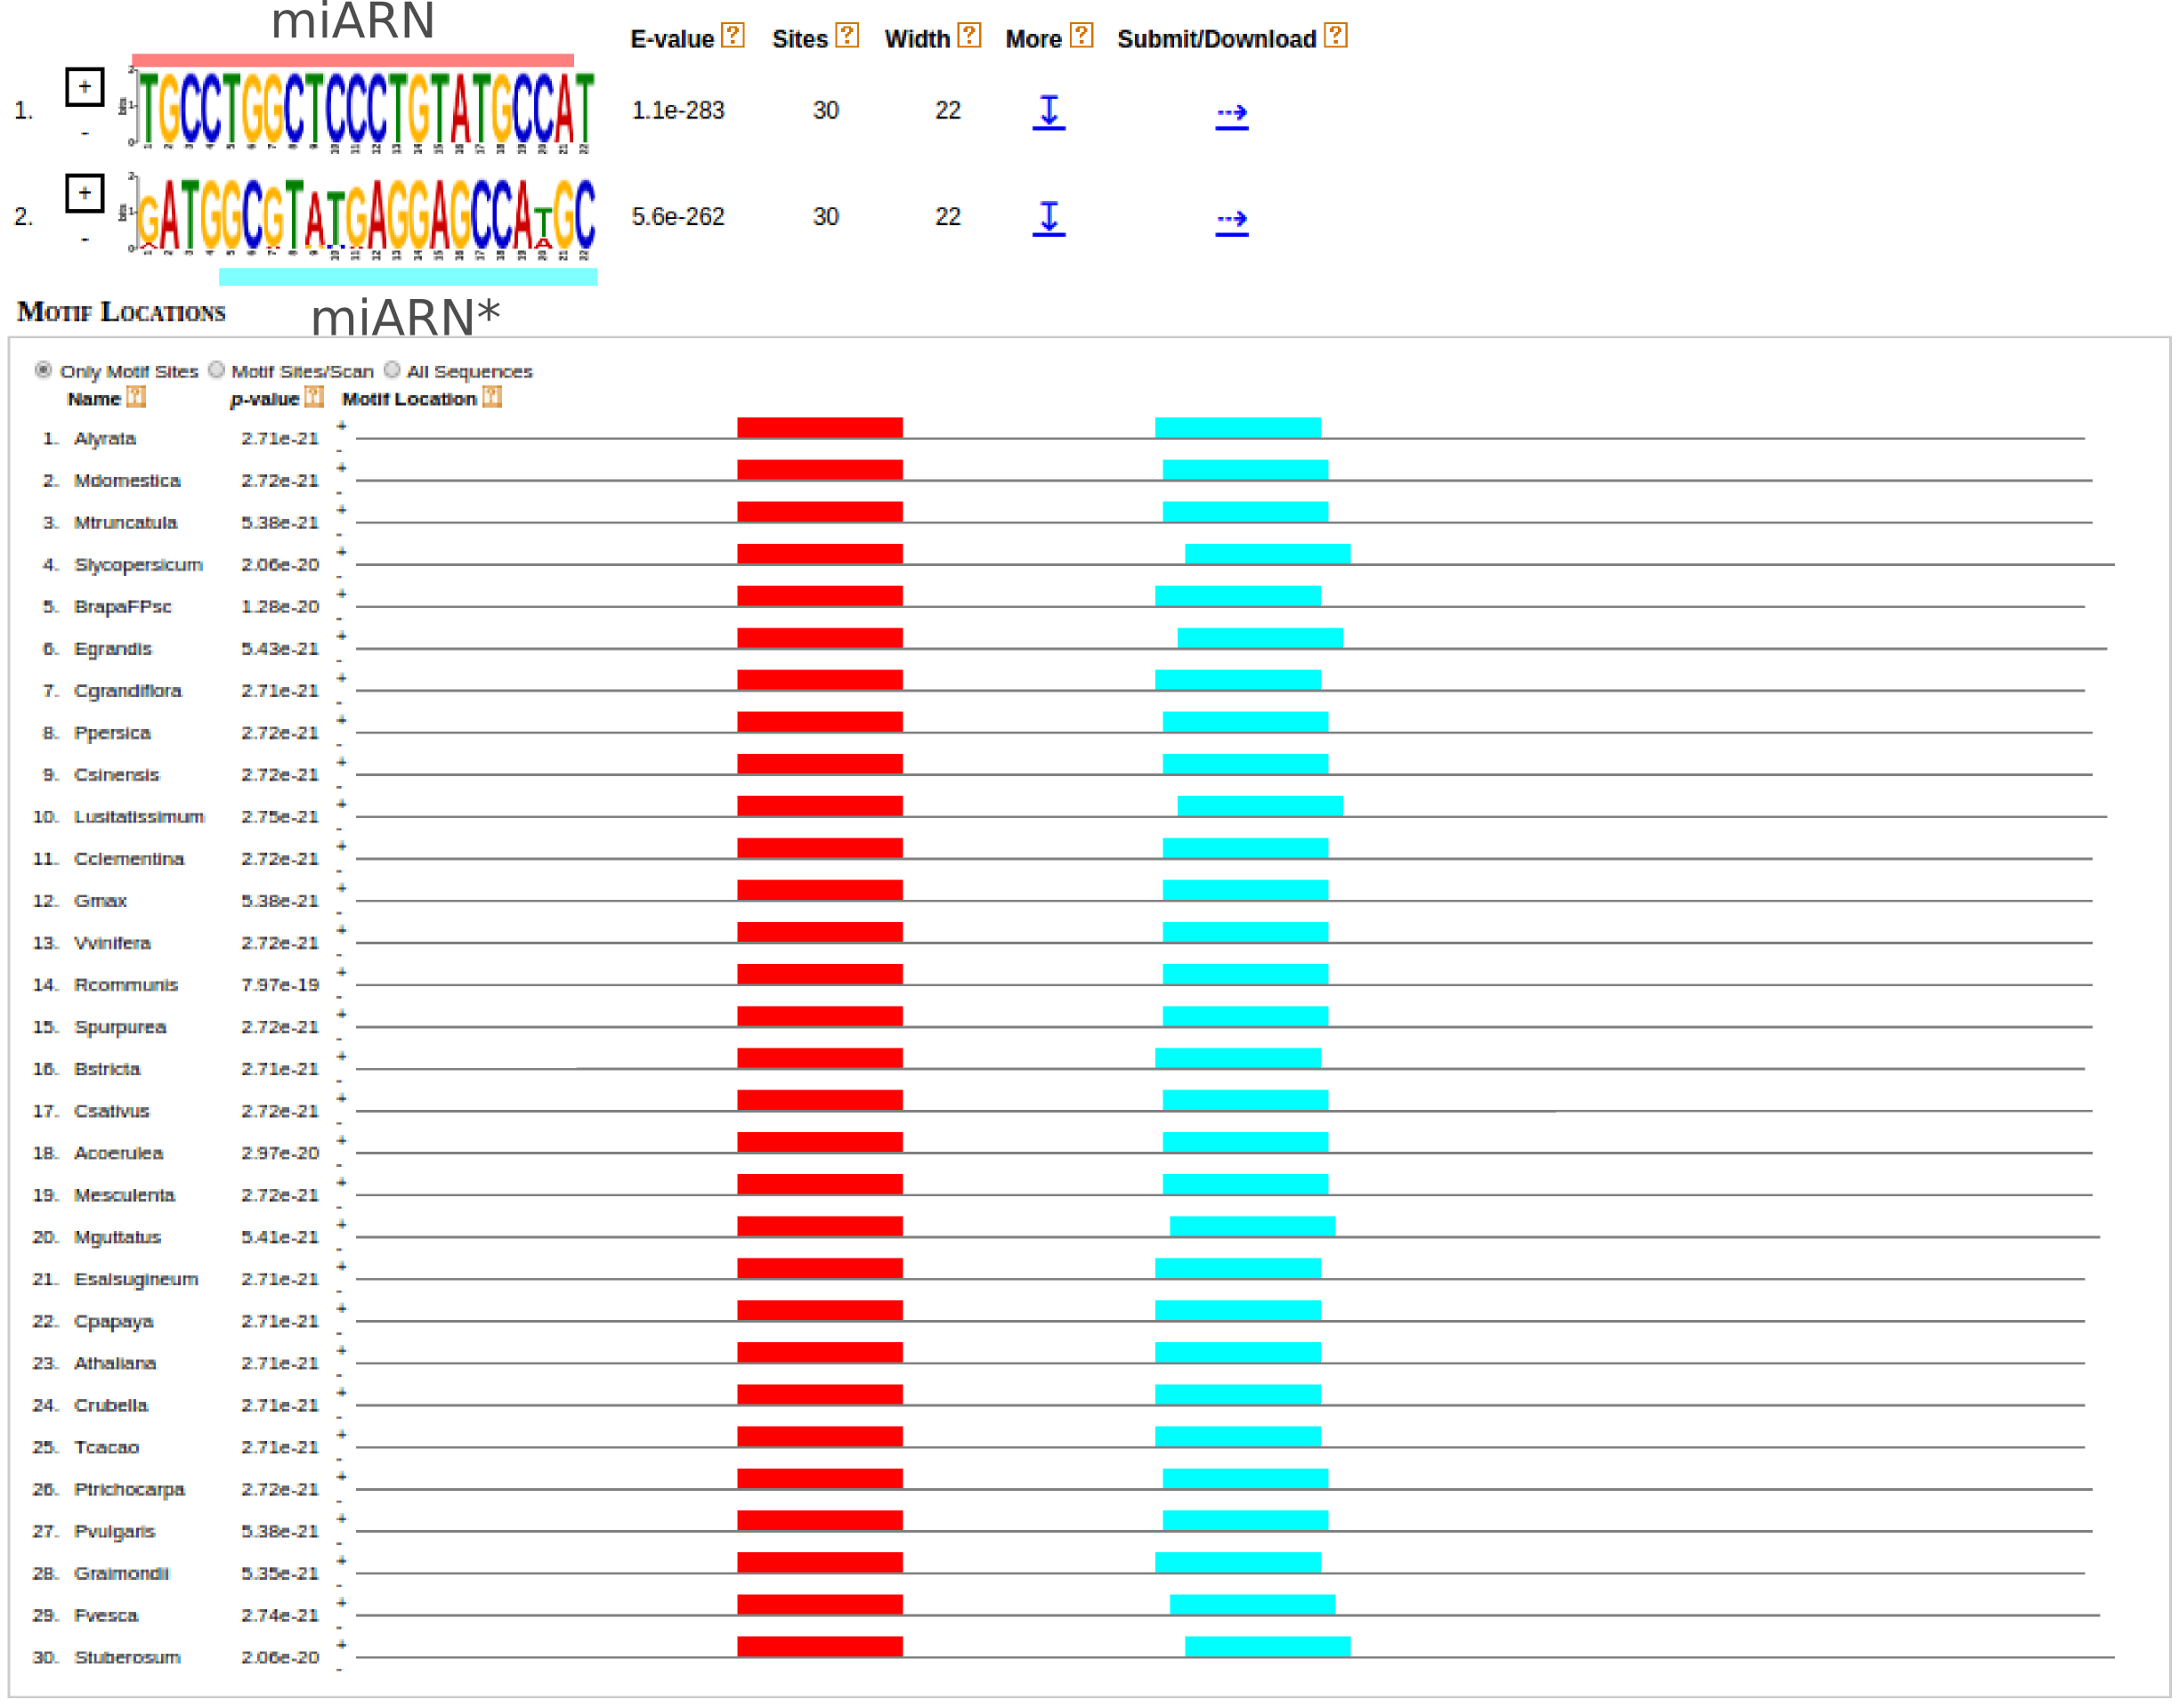
\includegraphics[width=.8\textwidth]{img/miR160a_meme.png}
	\end{center}
\end{frame}

\begin{frame}{En precursores que se procesan desde la base, el tamaño del tallo superior y al loop es muy variado en distintas especies}
	\begin{center}
		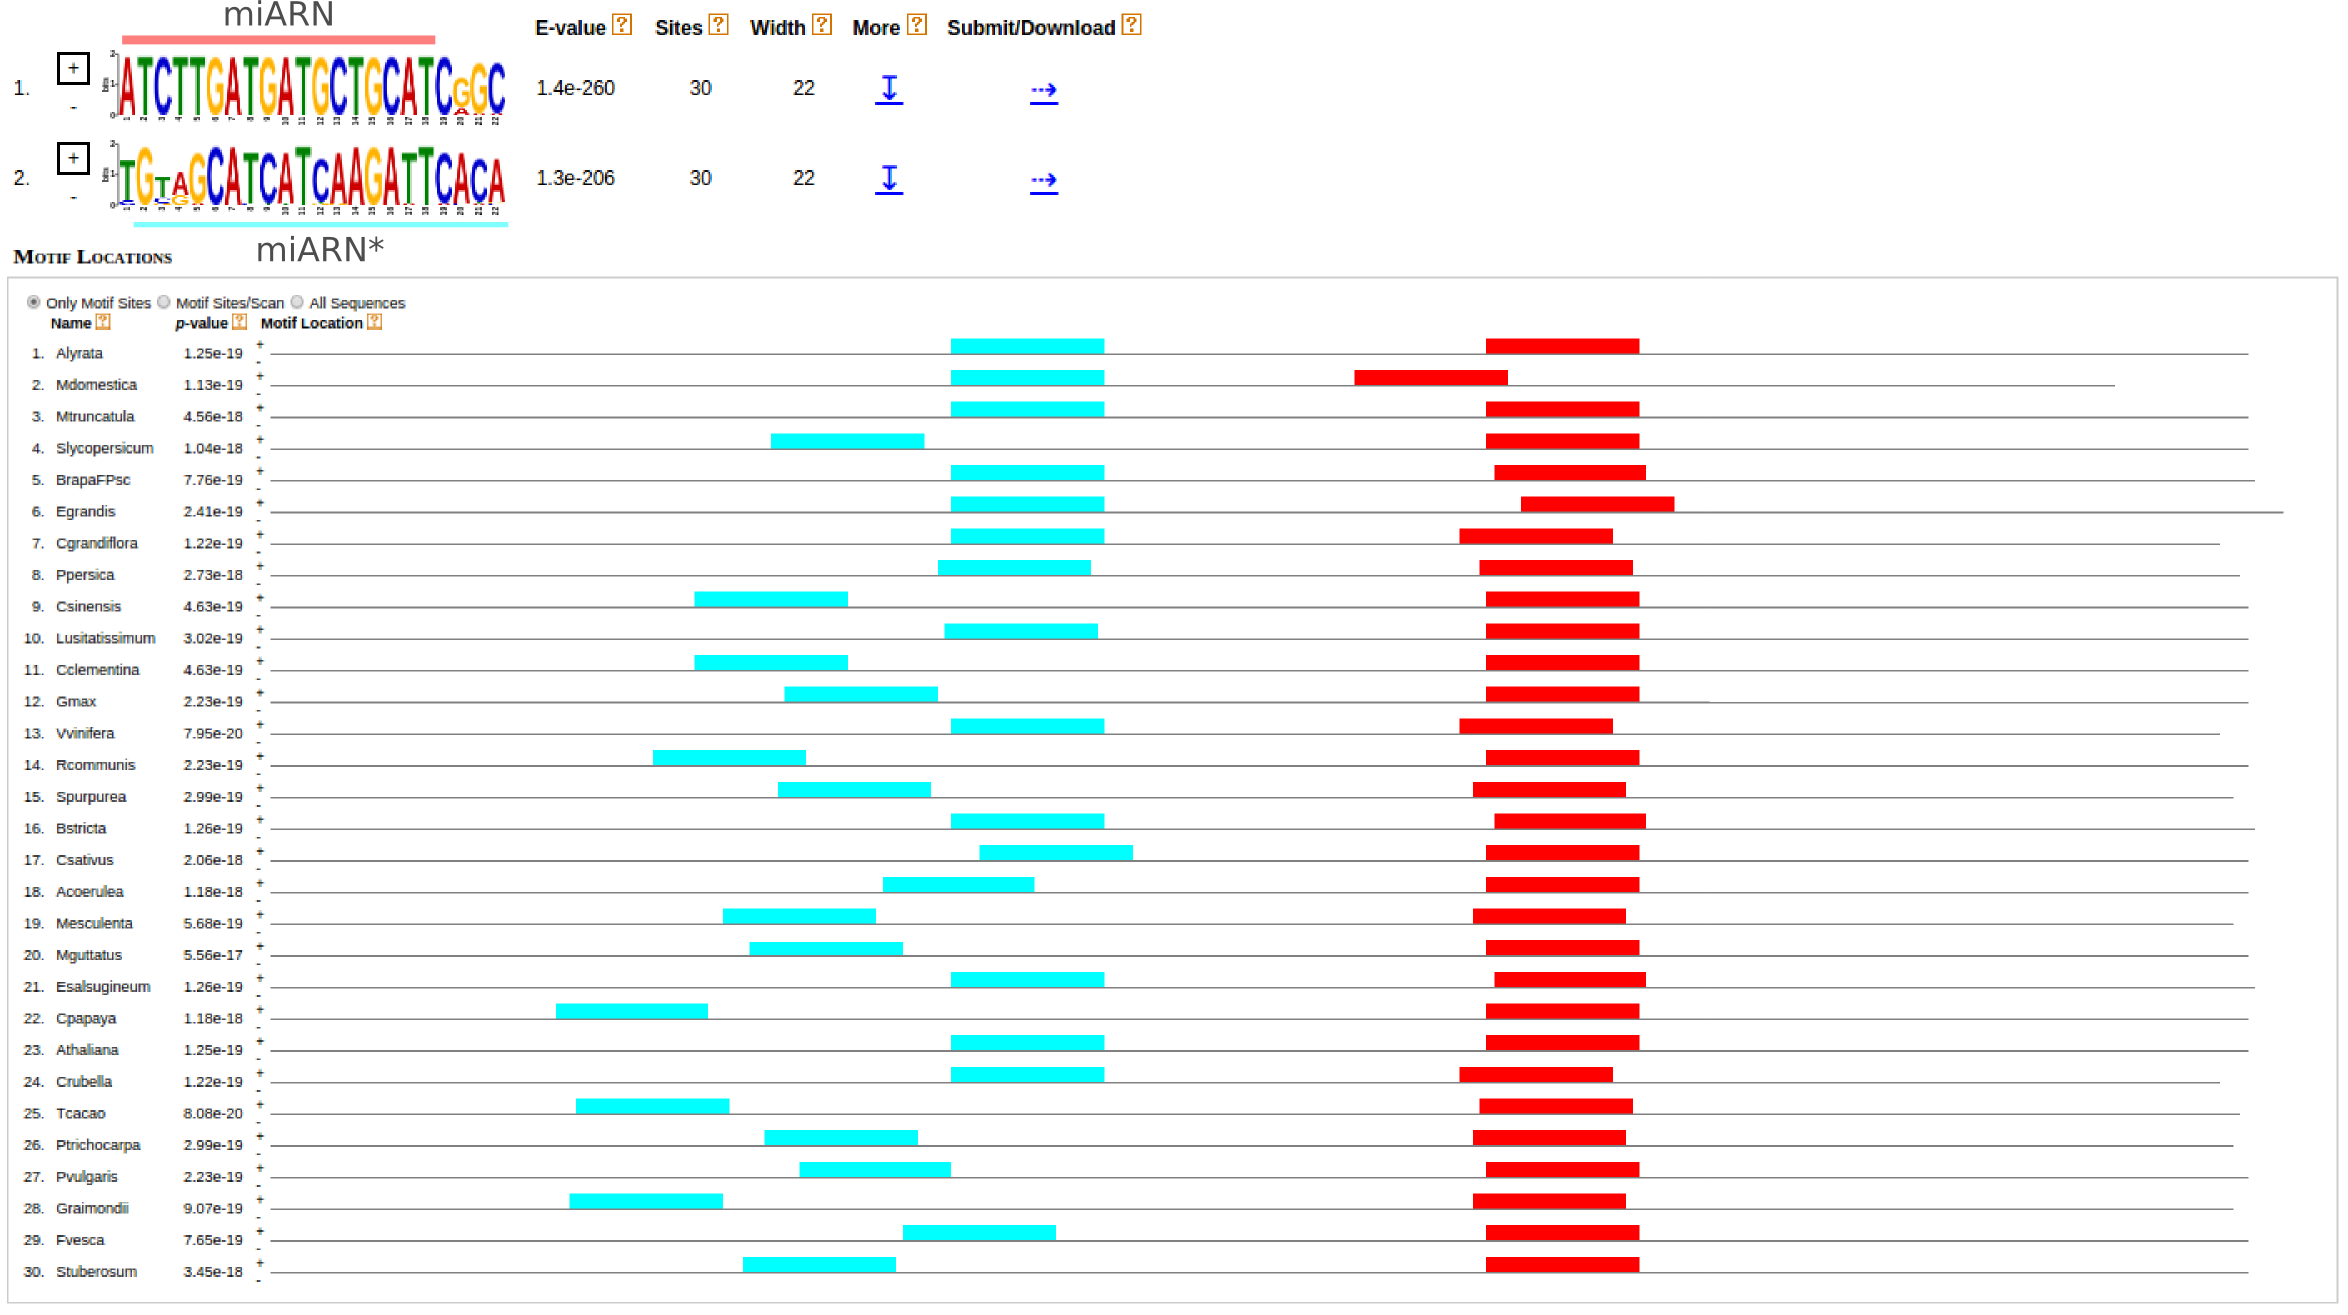
\includegraphics[width=1\textwidth]{img/miR172_meme.png}
	\end{center}
\end{frame}



\section{Conclusiones}

    %~ \vspace{1cm}

\begin{frame}{}
	\begin{center}
		\Huge Muchas gracias.
	\end{center}
\end{frame}

\begin{frame}{}
	\begin{center}
	\end{center}
\end{frame}


\begin{frame}{}
	\begin{center}
		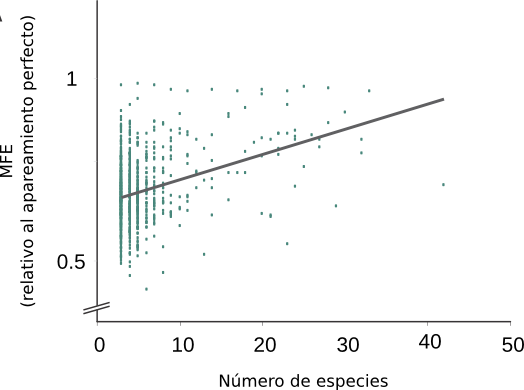
\includegraphics[width=.5\textwidth]{img/extras/NAR_fig3A.png}
	\end{center}
\end{frame}

\begin{frame}{}
	\begin{center}
		\includegraphics[width=.5\textwidth]{img/extras/NAR_fig3B.png}
	\end{center}
\end{frame}

\end{document}
